\documentclass[12pt,a4paper]{report}

% ----- packages -----
\usepackage{graphics}
\usepackage{head,fullpage,epsf,graphicx,amstext,url}
%\usepackage{mathtools} 
\usepackage{amssymb}
\usepackage{amsmath}
\usepackage{units}
\usepackage{afterpage}
\usepackage[caption=true]{subfig}

\newcommand\blfootnote[1]{%
  \begingroup
  \renewcommand\thefootnote{}\footnote{#1}%
  \addtocounter{footnote}{-1}%
  \endgroup
}


% ----- user defined commands -----
\newcommand{\msbar}{{\text{\tiny ${\overline{MS}}$ }} }
\newcommand{\order}[1]{\mathcal{O}({#1})}
\newcommand{\paren}[1]{ \left( {#1} \right) }
\newcommand{\bracket}[1]{ \left[ {#1} \right] }
\newcommand{\braces}[1]{ \left\{ {#1} \right\} }
\newcommand{\psibar}{ \overline{\psi} }
\newcommand{\boost}{{\text{\tiny $\Box$}}}
\newcommand{\bare}{{\text{\tiny $0$}}}
\newcommand{\one}{{\text{\tiny ${\rm I}$}}}
\newcommand{\two}{{\text{\tiny ${\rm II}$}}}
\newcommand{\three}{{\text{\tiny ${\rm III}$}}}
%\newcommand{\qqbar}{{\text{\tiny $q\bar{q}$}}}
\newcommand{\qqbar}{{q\bar{q}}}

\interfootnotelinepenalty=10000

\begin{document}

\thispagestyle{empty}

%                       This is a basic LaTeX Template
%                       for the MSc Dissertation report
%
\parindent=0pt          %  Switch off indent of paragraphs 
\parskip=5pt            %  Put 5pt between each paragraph  
%
%                       This section generates a title page
%                       Edit only the sections indicated to put
%                       in the project title, and submission date
%

\vspace*{0.1\textheight}

\begin{center}
        \huge{\bfseries Determining the Strong Coupling Constant using Lattice QCD}\\
\end{center}

\bigskip

\begin{center}
        \large{Matthew Inglis-Whalen}\\      % Author
        \bigskip
        \large{August 22, 2014}        % Submission Date
\end{center}

\vfill
%\vspace*{0.4\textheight}

\begin{center}
        
\includegraphics[width=35mm]{crest.pdf}
\end{center}

\medskip

\begin{center}

\large{
  MSc in Theoretical Physics\\[0.8ex]
  The University of Edinburgh\\[0.8ex]
  2014
}

\end{center}

\newpage


\pagenumbering{roman}

\begin{abstract}

A determination of $\alpha_\msbar^{(n_f=5)}(m_Z)$ is presented using $n_f=0$ and $n_f=2$ lattice data taken from the literature.
Closely following previous work by the QCDSF-UKQCD Collaboration, the main motivation for this paper is a newly determined value for 
the Sommer parameter $r_0$, as well as recently updated values of the inverse lattice spacing $r_0/a$. It is found that 
$\alpha_\msbar^{(n_f=5)}(m_Z)=0.1146 \pm 0.0016$, in tension with the current world average. 

\end{abstract}

\pagenumbering{roman}

\tableofcontents
\listoftables
\listoffigures

\begin{titlepage}
\vspace*{2in}
% an acknowledgements section is completely optional but if you decide
% not to include it you should still include an empty {titlepage}
% environment as this initialises things like section and page numbering.
%\section*{Acknowledgements}

\begin{center}

I would like to thank Dr. Roger Horsley for our many talks throughout the summer.
His experience was highly beneficial to my understanding of Lattice QCD, and his supervision key to the completion of this
work within the short time frame.

\vspace{240pt}

$\sim$ \textit{The devil's in the details} $\sim$

\end{center}

\end{titlepage}

\pagenumbering{arabic}









\chapter{Introduction}
\section{Motivation}
The quantum field theory describing the interactions of coloured particles, commonly known as Quantum
Chromodynamics (QCD), is built from the requirement that the standard model (SM) Lagrangian density 
must be locally invariant under any $SU(3)$ transformation acting on quark field colour indices. The 
theory exhibits two important characteristics: asymptotic freedom and confinement. 
\emph{Asymptotic freedom} is the qualitative observation that at high energies QCD becomes weakly coupled, 
allowing for accurate physical predictions through the use of perturbation theory. Conversely, 
\emph{confinement} describes the observation that at low energies QCD becomes strongly coupled, which 
precludes the use of perturbation theory and thus requires a non-perturbative approach. 

In energy regimes where perturbation theory applies, physical quantities are calculated by summing Feynman diagrams
for the relevant process. The final result is expressed as a truncated series expansion in powers of the \emph{strong coupling
 constant}, $\alpha_s$. Truncating the series at higher powers of $\alpha_s$ gives increasingly accurate results, 
with the stumbling block being that higher order terms in the series are exponentially more difficult to calculate. 
Yet even if the expansion coefficients were known to all orders, the degree of precision currently placed on $\alpha_s$ is not sufficient
to justify keeping terms with more than 3 powers of $\alpha_s$ above leading order (NNNLO). The current world average for the strong
coupling constant is \cite{PDG}
\begin{equation} \label{eq:alpha_world_average} \begin{aligned}
\alpha_s(m_Z)=0.1185 \pm 0.0006 ,
\end{aligned} \end{equation}

which means that even at the energy scale of the Z boson mass, where $\alpha_s$ is most precisely known, the NNNLO term is already of 
the same magnitude as the error on the LO term. This should be compared to the precision of the coupling constant in Quantum 
Electrodynamics (QED), which allows QED series expansions to be kept to 5 loops above leading order before the leading order error 
drowns out the N$^{5}$LO contributions.

For low-energy regimes such as those encountered in hadrons, Lattice QCD (LQCD) is currently the most popular non-perturbative
approach to calculating physical observables. Pioneered in 1974 by Kenneth G. Wilson with his seminal paper ``Confinement of Quarks''
\cite{Wilson:1974}, the method works by reformulating continuum QCD on a four-dimensional hypercubic lattice, allowing the quantum
vacuum to be simulated non-perturbatively through the use of Monte Carlo methods. By measuring vacuum expectation values of relevant
operators on the lattice and taking the continuum limit\footnote{By construction, in the limit that the lattice spacing $a \rightarrow 0$, 
the discretized theory reduces to the continuum theory.}, physical quantities such as masses and magnetic 
moments of hadrons can be extracted to high precision. The lattice method has been hugely successful in verifying \cite{Durr:2008} and even 
predicting \cite{Allison:2004,Abulencia:2005} experimental results, lending good credence to the belief that QCD describes the hadronic world.

These high precision non-perturbative techniques of Lattice QCD offer an enticing way to improve upon the current precision 
of the strong coupling constant. The goal of this work is to draw lattice data from the literature with the goal of calculating
the perturbative expansion parameter $\alpha_s$.

\section{Terminology}

In the real world, we know that quarks come in 6 different flavours: up, down, charm, strange, truth, and beauty. In practice, 
most calculations in QCD employ effective theories to integrate out the spurious degrees of freedom that are introduced
when including quark flavours that do not participate in a particular process \cite{VanKolck:2002}. This approach works because the 
process of renormalization introduces an energy scale $\mu$, resulting in the suppression of quark loops involving a quark with mass 
$m_q > \mu$. Consequently, most variables in QCD are dependent on $n_f$, an effective field theory parameter that counts the 
number of quarks with mass $m_q < \mu$. In this work, lattice data is drawn from lattice simulations where $n_f=0$ or $n_f=2$.

The central focus of this work is the strong coupling constant $\alpha_s$, which depends both on the scale $\mu$ and the
number of active fermions $n_f$. By convention, the quoted value is for $n_f=5$ and the scale is taken to be at the mass
of the Z boson. Moreover, the name ``strong coupling constant'' is decidedly ambiguous -- the expansion parameter $\alpha_s$ 
depends on the chosen scheme used for renormalization. The value of $\alpha_s$ given in eq. (\ref{eq:alpha_world_average}) is 
in the $\overline{MS}$ scheme, the most popular renormalization scheme used in QCD. This work uses multiple renormalization schemes,
and accordingly the expansion parameter in a particular scheme will hereafter be clearly labelled by $\alpha_S$.

\section{Context For This Work}

The specific methods used in this work were previously implemented by the QCDSF-UKQCD collaboration 
\cite{Booth:2001,Booth:2002,Gockeler:2004,Gockeler:2005}, however in the intervening 
time an updated value for the Sommer parameter $r_0$ has been published \cite{Bali:2012}. It has also come to light that the 
$n_f=2$ lattice data contained $r_{0}/a$ values that were too small \cite{Leder:2010,Aoki:2013}. This work closely follows the method 
of \cite{Gockeler:2005}, but contributes an exact closed form expression for the integral of the renormalization group equation, 
modifies an existing method of crossing the strange threshold, and updates the value for $\alpha_\msbar$ based on the new values 
for $r_0$ and $r_{0}/a$. 

It should be noted that the datasets herein, collected from the literature, are from studies using $n_f=0$ and $n_f=2$ active fermions, 
whereas current state-of-the-art studies use lattice configurations with $n_f=2+1$ \cite{McNeile:2010,Bazavov:2014} and even $n_f=2+1+1$ 
\cite{Blossier:2011,Blossier:2013}. Due to the complications involved with crossing the strange threshold, these many flavour simulations
are better suited to precision measurements of $\alpha_\msbar^{(n_f=5)}(m_Z)$. Accordingly, this work 
is primarily motivated by the updated $r_0$ and $r_{0}/a$ values, and is not meant to reflect the current capabilities of Lattice QCD. 

The structure of this paper is organized as follows. Chapter \ref{sec:theory} showcases the mathematics used to extract results from 
the lattice data. Chapter \ref{sec:data_and_results} tabulates the data taken from various sources in the literature and reveals the results
that can be drawn from the data. Chapter \ref{sec:discussion} discusses the overall quality level of this paper, and takes a look
at how the results presented here agree with values from the literature. Chapter \ref{sec:conclusions} recapitulates the work, and
concludes.












\chapter{Theory} \label{sec:theory}
The goal of this chapter is to elucidate the concepts and methods required to calculate $\alpha_\msbar$ 
from lattice data. Rather than presenting the material in the order in which calculations take place, an attempt has been made
to put concepts in an order which should make sense to a reader not familiar with Lattice QCD. To begin, \S\ref{sec:lattice_details} 
outlines the quantum action used to generate the datasets tabulated in Chapter \ref{sec:data_and_results}, and introduces the Sommer 
parameter $r_0$. In \S\ref{sec:scale_dependence}, the scale dependence of $\alpha_S$ is determined by integrating the beta function, 
which introduces the fundamental $\Lambda$ parameter. For renormalization schemes where the four loop beta function coefficient 
$\beta_3^S$ is not known, a method for estimating its value is described. In \S\ref{sec:converting_schemes}, equations are presented 
for determining $\alpha_\msbar$ when the coupling constant $\alpha_S$ is known in another scheme. Particular attention is paid to the 
bare lattice scheme and the boosted coupling scheme. \S\ref{sec:three_methods} presents three methods that each allow for the 
determination of the continuum $\Lambda_{(0)}$ and $\Lambda_{(2)}$ parameters from the bare lattice data. Finally, 
\S\ref{sec:crossing_thresholds} details the intricacies of running $\alpha_\msbar$ up to the mass of the Z-boson. By matching the 
force between static quarks across the strange threshold, it is shown how $\Lambda_{(3)}^\msbar$ may be determined using 
$\Lambda_{(0)}^\msbar$ and $\Lambda_{(2)}^\msbar$ as input. It is then shown how the charm and beauty thresholds are crossed by 
writing down a perturbative expression for the discontinuity of $\alpha_\msbar$ at the relevant matching scales.

\section{Lattice Details} \label{sec:lattice_details}

While no lattice simulations were performed by the author in the completion of this work, it remains necessary to briefly outline 
some definitions and variables used to generate vacuum configurations and calculate quantities on the lattice.

\subsection{The Lattice Action} \label{sec:lattice_action}

All simulations use the standard gauge field action \cite{Booth:2001}
\begin{equation} \label{eq:guage_action} \begin{aligned}
\mathcal{S}_{G} &= \beta \sum\limits_{x \in \Lambda} \frac{1}{3} \mathrm{Tr} \paren{ U_{\boost}(x) } ,
\end{aligned} \end{equation}
where $\beta \equiv 3/2\pi\alpha_0 $, not be confused with the beta function, fixes the coupling constant in the bare
lattice scheme (denoted by the `0' subscript). The sum is over the set of lattice sites, and $U_\boost$ is the plaquette,
the sum over all nearest-neighbour Wilson loops originating from lattice site $x$.

When fermions are put on the lattice Wilson fermions are used, which come equipped with the action \cite{Gattringer:2010}
\begin{equation} \label{eq:wilson_action} \begin{aligned}
\mathcal{S}_{\rm Wilson} &=a^4 \sum\limits_{f=1}^{n_f} \sum\limits_{x,y \in \Lambda} \psibar^{(f)}(x) D^{(f)}(x,y;U)\psi^{(f)}(y) ,
\end{aligned} \end{equation}

where $D^{(f)}(x,y;U)$ is Wilson's lattice Dirac operator. As in the continuum theory, the lattice Dirac operator
contains a term proportional to the bare quark mass $a m_q$, which is commonly paramaterized by the hopping parameter
$\kappa$ and its critical value $\kappa_c$ via the relation
\begin{equation} \label{eq:amq_relation} \begin{aligned}
am_q = \frac{1}{2}\paren{\frac{1}{\kappa}-\frac{1}{\kappa_c}} .
\end{aligned} \end{equation}

The Wilson fermion action suffers from $\order{a}$ discretization errors, which can be removed by using the $\order{a}$ 
improved Sheikholeslami-Wohlert (clover) action \cite{Gattringer:2010,Luscher:1998,Sheikholeslami:1985}
\begin{equation} \label{eq:clover_action} \begin{aligned}
\mathcal{S}_{\rm clover} &=i c_{sw}\frac{a^5}{4} \sum\limits_{x \in \Lambda} \psibar(x) \sigma_{\mu\nu} F_{\mu\nu}(x) \psi(x).
\end{aligned} \end{equation}

The Sheikholeslami-Wohlert coefficient has been determined non-perturbatively, and is best described by the rational equation 
\cite{Luscher:1998,Jansen:1997}

\begin{equation} \label{eq:c_sw_alpha} \begin{aligned}
c_{sw}(\alpha_\bare) &=\frac{1-5.705\alpha_\bare - 27.63\alpha_\bare^2 + 23.81\alpha_\bare^3 +1122\alpha_\bare^4}{1-9.048\alpha_\bare} .
\end{aligned} \end{equation}

\subsection{The Sommer Parameter $r_0$} \label{sec:sommer_parameter}

One of the most important variables used in this paper is the Sommer parameter $r_0$ \cite{Sommer:1993}. In general, lattice calculations
use dimensionless parameters (e.g. masses $a m_q$, $a m_\pi$, $a\mu$ and lengths $r/a$, $L/a$ ), so a physical 
quantity is needed to make a connection to the real world. $r_0$ provides one possible method for setting the physical scale of 
lattice calculations. The definition of $r_0$ is given in terms of the force $f(r)$ between two static quarks, and is expressed as
\begin{equation} \label{eq:r0_def} \begin{aligned}
r_0^2 f(r_0) = 1.65 .
\end{aligned} \end{equation}

A recent determination of $r_0$ \cite{Bali:2012} gives the value that will be used in this work,
\begin{equation} \label{eq:r0_value} \begin{aligned}
r_0 &= 0.501(10)(11)\ {\rm fm} \\
    &= 2.538(51)(56)\ {\rm GeV}^{-1} .
\end{aligned} \end{equation}

One particularly useful quantity related to $r_0$ is the ratio $r_0/a$. It can be calculated on the lattice independent from any knowledge
of $r_0$ itself \cite{Gattringer:2010}, and allows lattice quantities written in terms of an unknown lattice spacing $a$ to 
be rewritten in term of a known value $r_0$. $r_0/a$ is one of the few variables held in the datasets of this paper, and is central to 
the determination of $\Lambda_{(n_f)}^\msbar$, from which $\alpha_\msbar^{(n_f)}$ follows immediately, as is shown in the following 
section.






\section{Scale Dependence and the Lambda Parameter} \label{sec:scale_dependence}
In this section the scale dependence of $\alpha_S$ is introduced via the renormalization group equation, and it is 
shown how the beta function may be integrated analytically, giving rise to the fundamental parameter $\Lambda$. Rational 
approximants are then introduced as a way to estimate the 4-loop beta function coefficient in renormalization schemes where only 
three-loop results are known. 

\subsection{The Renormalization Group} \label{sec:renormalization_group}

The process of renormalizing QCD introduces a mass scale $\mu$ and an effective field theory parameter $n_f$ on which the parameters of 
the theory depend. These parameters are, namely, the strong coupling constant $\alpha_S(\mu;n_f)$ and the masses $m_q^S(\mu;n_f)$ of 
each of the quarks. Focusing on the scale dependence of $\alpha_S(\mu;n_f)$, the running of the strong coupling constant is governed 
by the QCD beta function. In an arbitrary scheme $S$, the beta function is defined via the renormalization group equation

\begin{equation} \label{eq:beta_def} \begin{aligned}
\frac{d\ \alpha_S^{(n_f)}(\mu)}{d \ln \mu^2} = -(\alpha_S^{(n_f)}(\mu))^2\sum\limits_{k=0}^{\infty}
 \beta_k^S(n_f)(\alpha_S^{(n_f)}(\mu))^k \equiv \beta^S(\alpha_S^{(n_f)}(\mu)) .
\end{aligned} \end{equation}

For the sake of brevity, the functional dependences of $\beta_k^S(n_f)$ and $\alpha_S^{(n_f)}(\mu)$ will hereafter be suppressed. In general, 
the coefficients $\beta_k$ are dependent on the scheme chosen to renormalize the theory; exceptionally, however, 
$\beta_0$ and $\beta_1$ are scheme independent. In the $\overline{MS}$ scheme the first four beta function coefficients 
are known \cite{vanRitbergen:1997,Czakon:2004}, and with the standard normalization of the $SU(3)$ generators, these coefficients are

\begin{equation} \label{eq:beta_coeffs} \begin{aligned}
\beta_0&=\paren{\frac{1}{4\pi}}  \bracket{\ 11-\frac{2}{3}n_f\ }                                                           \\
\beta_1&=\paren{\frac{1}{4\pi}}^2\bracket{\ 102-\frac{38}{3}n_f\ }                                                         \\
\beta_2^\msbar&=\paren{\frac{1}{4\pi}}^3\bracket{\ \frac{2857}{2}-\frac{5033}{18}n_f+\frac{325}{54}n_f^2\ }                       \\
\beta_3^\msbar&=\paren{\frac{1}{4\pi}}^4\left[\ \frac{149753}{6}+3564\zeta_3 -\paren{\frac{1078361}{162}+\frac{6508}{27}}n_f \right. \\
&\ \ \ \ \ \ \ \ \ \ \ \ \ \ \ \ \ \ \ \ \ \ \ \ \ \ 
\left. -\paren{\frac{50065}{162}+\frac{6472}{81}\zeta_3}n_f^2-\frac{1093}{729}n_f^3\ \right] ,
\end{aligned} \end{equation}

where, $\zeta_3 \approx 1.20205690$ is Riemann's zeta function evaluated at $z=3$. Integrating equation \ref{eq:beta_def} 
introduces an arbitrary integration constant that depends mostly on convention \cite{Monsay:1981}, but following the convention 
used by the FLAG Working Group \cite{Aoki:2013}, the solution to eq. (\ref{eq:beta_def}) is
\begin{equation} \label{eq:beta_integ_alpha} \begin{aligned}
\frac{\mu}{\Lambda_{n_f}^S}=\exp\paren{\frac{1}{2 \beta_0 \alpha_S}}\paren{\beta_0\alpha_S}^{\frac{\beta_1}{2\beta_0^2}}
\exp\bracket{\frac{1}{2}\int_{0}^{\alpha_S} d\alpha' \paren{\frac{1}{\beta(\alpha')}
+\frac{1}{\beta_0 \alpha'^2}-\frac{\beta_1}{\beta_0^2 \alpha'}}} .
\end{aligned} \end{equation}

If written in terms of the roots of the beta function, the integral in eq. (\ref{eq:beta_integ_alpha}) can be performed analytically to any 
finite order in perturbation theory. To one loop order, only $\beta_0$ is non-zero, and eq. (\ref{eq:beta_integ_alpha}) reduces to
\begin{equation} \label{eq:beta_integ_1loop} \begin{aligned}
\frac{\mu}{\Lambda_{(n_f)}^S}=\exp\paren{\frac{1}{2\beta_0\alpha_S }} ,
\end{aligned} \end{equation}

Before moving on to the general L-loop case, the integration constant $\Lambda_{(n_f)}^S$ should be given a better introduction. Equation 
(\ref{eq:beta_integ_1loop}) shows that in the limit $\mu \rightarrow \Lambda_{(n_f)}^S$, the coupling constant $\alpha_S \rightarrow \infty$,
making any perturbative expansion in $\alpha_S$ divergent. This limit is only strictly obeyed in the 1-loop case, but the 
qualitative behaviour remains the same for higher loop orders; as $\mu \rightarrow \Lambda_{n_f}^S$, $\alpha_S$ becomes large,
prohibiting its use as a perturbative expansion parameter. This is why perturbation theory fails to explain 
hadronic processes -- the typical energy scale of hadrons $\mu_{\rm had} \approx \Lambda_{(n_f)}^\msbar$, dooming any chance of 
writing down a convergent series in $\alpha_\msbar$ 

It should be made clear that $\Lambda_{(n_f)}^S$ is of central importance for determining $\alpha_S$. It is the only parameter 
that determines how $\alpha_S$ runs with scale $\mu$, and thus can be considered more fundamental than $\alpha_S$ itself. Once
$\Lambda_{(n_f)}^S$ is known, $\alpha_S^{(n_f)}(\mu)$ can be easily determined. Consequently, the majority of this work's
analysis focuses on determining physical $\Lambda_{(0)}^\msbar$ and $\Lambda_{(2)}^\msbar$, and extrapolating those values to
$n_f=5$.

To higher orders, the integration procedure depends on finding the roots of the beta function. Letting $N$ denote the index of the last 
non-vanishing coefficient $\beta_k$, the Abel-Ruffini theorem implies that this factorization can be done algebraically for 
$N \le 4$ (up to 5 loops). For $N \ge 5$, the root-finding must be done numerically. Rewriting the beta function in terms of 
its non-zero roots $r_k$
\begin{equation} \label{eq:beta_roots} \begin{aligned}
\beta^S(\alpha_S)&=-\beta_N \alpha_S^2\prod\limits_{k=1}^{N} (\alpha_S-r_k) ,
\end{aligned} \end{equation}

then the partial fraction decomposition for the reciprocal of this rewritten beta function is
\begin{equation} \label{eq:partial_fraction_N} \begin{aligned}
\frac{1}{-\beta_N \alpha_S^2}\prod\limits_{k=1}^{N} \frac{1}{\alpha_S-r_k}=\frac{A}{\alpha_S}+\frac{B}{\alpha_S^2}
+\sum\limits_{k=1}^{N}\frac{P_k^S}{\alpha_S-r_k} ,
\end{aligned} \end{equation}

with

\begin{equation} \label{eq:partial_fraction_N_coeffs} \begin{aligned}
A&=\frac{(-1)^{N+1}}{\beta_N}\bracket{\prod\limits_{k=1}^{N}\frac{1}{r_k}}\bracket{\sum\limits_{k=1}^{N} \frac{1}{r_k}} \\
B&=\frac{(-1)^{N+1}}{\beta_N}\prod\limits_{k=1}^{N} \frac{1}{r_k} \\
P_k^S&=-\frac{1}{\beta_N r_k^2}\prod\limits_{\substack{j=1 \\ j \neq k}}^{N} \frac{1}{r_k-r_j} .
\end{aligned} \end{equation}

By multiplying out the product in eq. (\ref{eq:beta_roots}) and collecting powers of $\alpha_S$, it can be shown that the expressions for 
$A$ and $B$ simplify to $A=\beta_1/\beta_0^2$ and $B=-1/\beta_0$. These values for $A$ and $B$ allow the singular terms of eq. 
(\ref{eq:beta_integ_alpha}) to be exactly cancelled, regardless of expansion order. Using these results, eq. (\ref{eq:beta_integ_alpha}) may be 
written as
\begin{equation} \label{eq:beta_integ_NLloop} \begin{aligned}
\frac{\mu}{\Lambda_{(n_f)}^S}=\exp\paren{\frac{1}{2\beta_{0}\alpha_S }} (\beta_0\alpha_S)^{\frac{\beta_1}{2\beta_0^2}} 
                    \, \prod\limits_{k=1}^{N} \paren{1-\frac{\alpha_S}{r_k}}^{\frac{P_k^S}{2}}  .
\end{aligned} \end{equation}

This expression holds provided none of the roots $r_k$ are repeated. The nonzero roots of the beta function are, in general, complex, 
but the imaginary component of eq. (\ref{eq:beta_integ_NLloop}) vanishes exactly, as it must for a purely real integral. One should 
be aware, however, that computational rounding errors can introduce a small imaginary component when evaluating the expression 
numerically. Taking the real part of the result solves any problems that may be connected to this issue. 

For later convenience, the RHS of eq. (\ref{eq:beta_integ_NLloop}) is defined as the function
\begin{equation} \label{eq:M_of_alpha} \begin{aligned}
M_{(n_f)}^S(\alpha_S)=\exp\paren{\frac{1}{2\beta_{0}\alpha_S }} (\beta_0\alpha_S)^{\frac{\beta_1}{2\beta_0^2}} 
                    \, \prod\limits_{k=1}^{N} \paren{1-\frac{\alpha_S}{r_k}}^{\frac{P_k^S}{2}} .
\end{aligned} \end{equation}

Unfortunately, $M^S(\alpha_S)$ cannot be inverted analytically to solve for $\alpha_S(\mu)$. Some researchers 
iteratively invert the expression by writing $\alpha_S(\mu)$ as a series expansion in inverse powers of $\ln (\mu/\Lambda_{n_f}^S)$ 
\cite{PDG,Monsay:1981}, but for the purposes of this paper a numerical inversion is sufficient.

\begin{figure}[h]
\begin{center}
  \vspace{-10pt}
  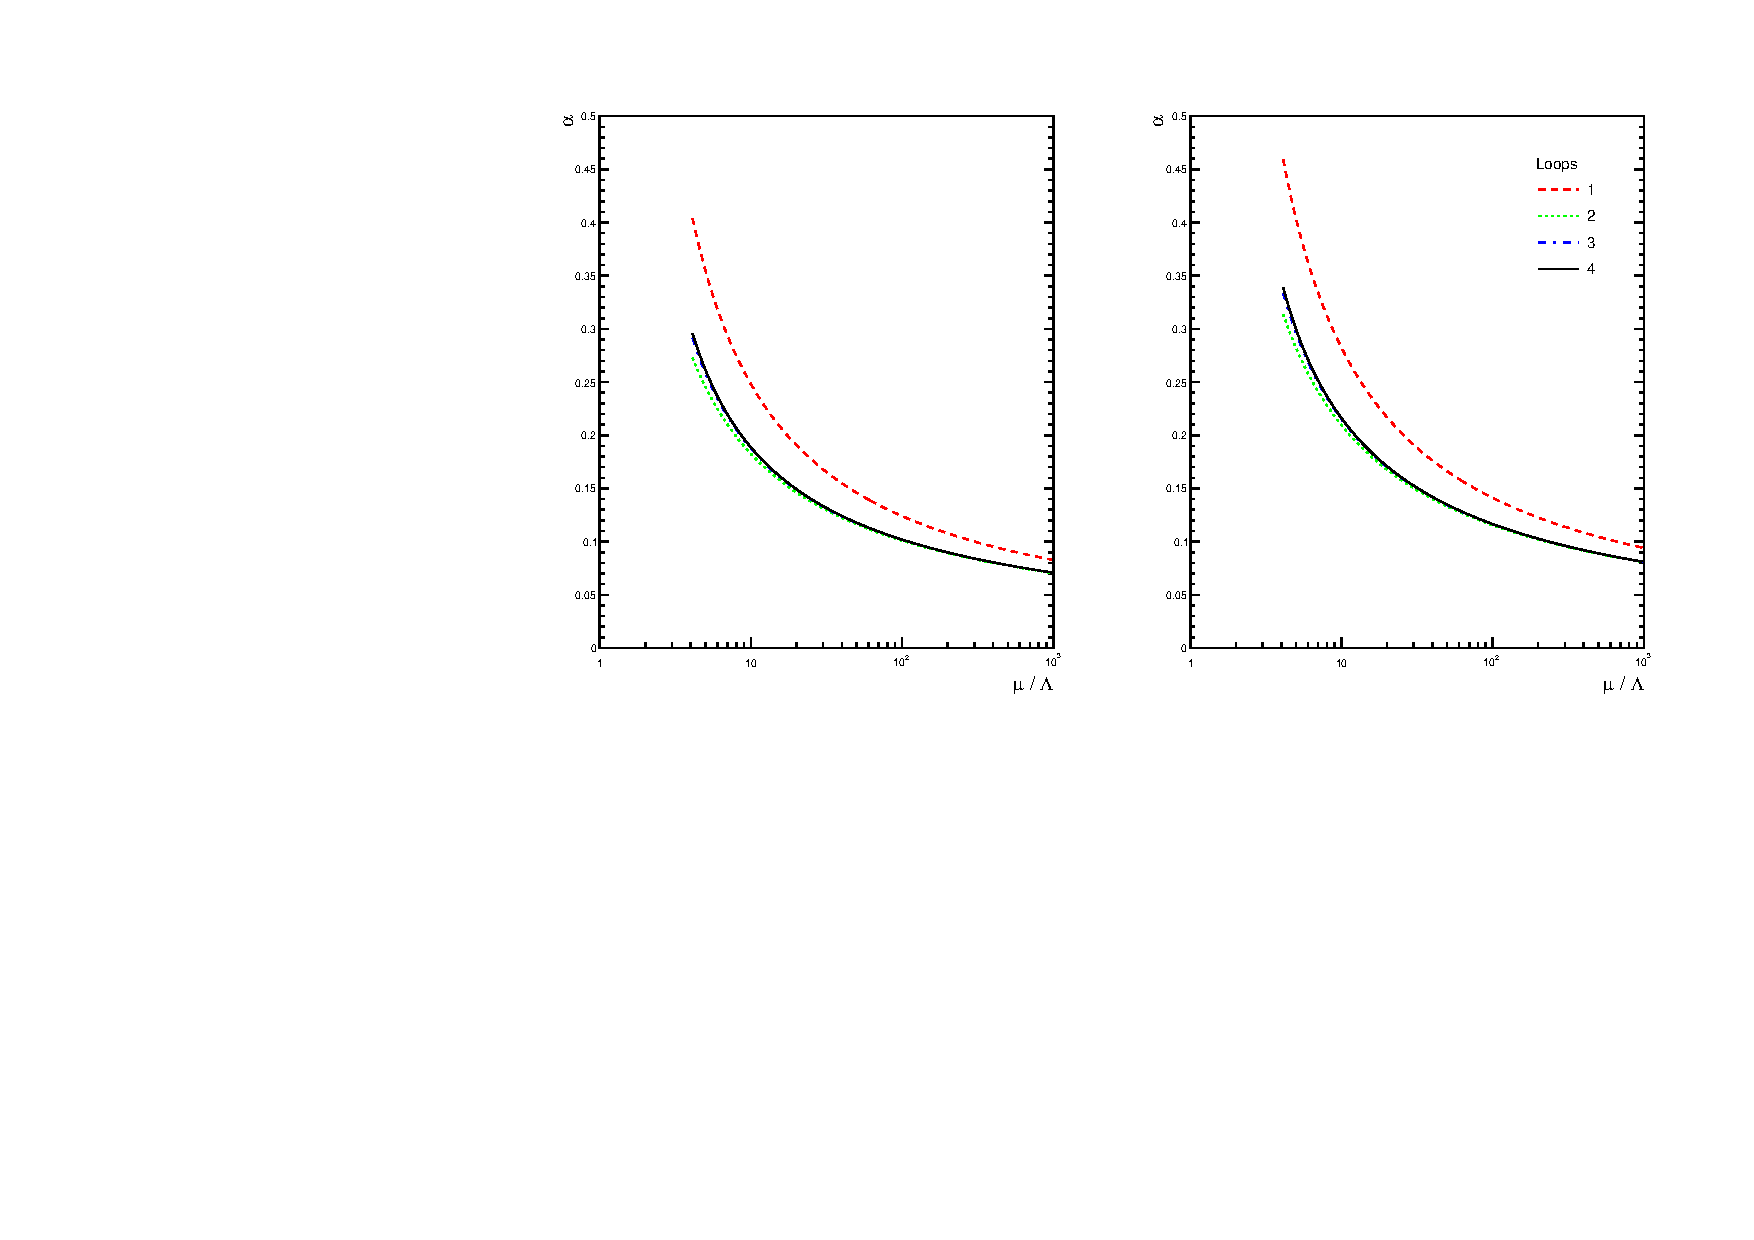
\includegraphics[width=5.5in]{alpha_of_mu_analytic.pdf}
  \caption{$\alpha_\msbar$\ \ vs. $\mu / \Lambda_{(n_f)}^\msbar$ for $n_f=0$ (left) and $n_f=2$ (right), using increasingly 
higher orders in the perturbative expansion of the beta function.  }
  \label{fig:alpha_of_mu}
\end{center}
\end{figure}

In \S\ref{sec:converting_schemes}, the series expansion of the natural logarithm of eq. (\ref{eq:M_of_alpha}) is required to derive a 
useful result. From the asymptotic relation \cite{Christou:1998}
\begin{equation} \label{eq:asymptotic_relation} \begin{aligned}
M_{(n_f)}^S(\alpha_S)=\exp\paren{\frac{1}{2\beta_{0}\alpha_S }} (\beta_0\alpha_S)^{\frac{\beta_1}{2\beta_0^2}} 
                    \paren{1-q\alpha_S+\order{\alpha_S^2}} ,
\end{aligned} \end{equation}

where 
\begin{equation} \label{eq:asymptotic_scaling_constant} \begin{aligned}
q=\frac{\beta_1^2-\beta_0\beta_2^S}{2\beta_0^3} ,
\end{aligned} \end{equation}

it can easily be seen that 
\begin{equation} \label{eq:asympototic_equality} \begin{aligned}
\sum\limits_{k=1}^{N} \frac{P_k^S}{2} \ln \paren{1-\frac{\alpha_S}{r_k^S}} = \ln \paren{1-q\alpha_S+\order{\alpha_S^2}} .
\end{aligned} \end{equation}

By expanding the natural logarithm in its power series and matching powers of $\alpha_S$, the identity
\begin{equation} \label{eq:asymptotic_identity} \begin{aligned}
\sum\limits_{k=1}^{N} \frac{P_k^S}{2r_k} = q
\end{aligned} \end{equation}

is derived. This identity will play a key role in deriving a relation allowing the 3-loop beta function coefficient to be calculated
in the lattice and boosted coupling schemes.

\subsection{Pad\'{e} Approximants} \label{sec:pade_approximants}
In the overwhelming majority of renormalization schemes, the QCD beta function is not known to four-loop order. Rather than leaving
the beta function truncated to 3-loop order, the method of Pad\'{e} approximants \cite{Assche:2006} can be used to estimate
the 4-loop coefficient $\beta_3$. The goal is to sizably reduce the truncation error while minimizing any errors
that might be generated in this estimation procedure.

In general, if a function $f(x)$ is given by the \emph{true} Taylor series,
\begin{equation} \label{eq:fx_Taylor} \begin{aligned}
f(x) \approx \sum\limits_{i=0}^{\infty} c_{i} x^{i}
\end{aligned} \end{equation}

but the coefficients $c_{i}$ are only known up to some index $N$, then 
the ``best'' \cite{Walsh:1974} approximation of the function $f(x)$ is given by the $[L/M]$ Pad\'{e} approximant 
\begin{equation} \label{eq:fx_nm_pade} \begin{aligned}
f_{[L/M]}(x) \approx \frac{\sum\limits_{i=0}^{L} p_{i} x^{i}}{1+\sum\limits_{j=1}^{M} q_{j} x^{j}}  ,
\end{aligned} \end{equation}

where $L+M=N$. The coefficients $p_i$ and $q_j$ are constructed in such a way that when the denominator is expanded out, the resulting
coefficients of $x^n$ are pairwise equal to the coeffients $c_n$ for $n \le N$. The next coefficient of the true 
Taylor series expansion, $c_{N+1}$, is then estimated by the corresponding coefficient of $x^{N+1}$. 

Concretely, the 3-loop beta function is written
\begin{equation} \label{eq:beta_3_loop} \begin{aligned}
\beta^{S}(\alpha_S)=-\beta_0 \alpha_S^2 - \beta_1 \alpha_S^3 - \beta_2^S \alpha_S^4 ,
\end{aligned} \end{equation}

so the \emph{true} beta function is best estimated by the [3/1] Pad\'{e} approximant
\begin{equation} \label{eq:beta_31_pade} \begin{aligned}
\beta^{S}_{[3/1]}(\alpha_S)=-\frac{\beta_0 \alpha_S^2 + \paren{\beta_1 - \frac{\beta_0\beta_2^2}{\beta_1}} \alpha_S^3 }{1 - \frac{\beta_2^S}{\beta_1} \alpha_S}.
\end{aligned} \end{equation}

Expanding out the denominator of eq. (\ref{eq:beta_31_pade}) reveals that the Pad\'{e} approximant 
estimates $\beta_3 \approx \beta_2^2/\beta_1$. To lend confidence to this method, the true and estimated values of $\beta_3^\msbar$ are
given. For $n_f=0$, the true value of $\beta_3$ is 1.17, while the estimate is $\beta_2^2/\beta_1 = 0.80$. For $n_f=2$, the
exact value of $\beta_3$ is 0.68, while the Pad\'{e} method estimates $\beta_2^2/\beta_1 = 0.42$. Clearly the method leaves something
to be desired, but at least the values are on the same order of magnitude. This estimation procedure will be used in 
\S\ref{sec:three_methods}, where the beta function of the lattice scheme is known only to 3 loops.

Some experts \cite{Gockeler:2005} hold the Pad\'{e} approximation in high esteem, and in this author's opinion
give undue weight to the results produced using this estimation procedure. This paper takes a more conservative approach 
and will weight all results equally, whether Pad\'{e} improved or not.












\section{Converting Between Renormalization Schemes} \label{sec:converting_schemes}

In this work, three renormalization schemes are used: the $\overline{MS}$ scheme, the bare lattice scheme (denoted by the `0' subscript), 
and the \emph{boosted coupling} scheme (denoted by the `$\Box$' subscript). The bare lattice coupling $\alpha_\bare$ is put in by 
hand to the simulation, while the boosted coupling $\alpha_\boost$ is defined as \cite{Horsley:2008}
\begin{equation} \label{eq:boosted_coupling_def} \begin{aligned}
\alpha_\boost \equiv \frac{\alpha_\bare}{P}  ,
\end{aligned} \end{equation}

where 

\begin{equation} \label{eq:plaquette_def} \begin{aligned}
P \equiv \left< \frac{\mathrm{Tr}\ U_\boost}{3} \right>
\end{aligned} \end{equation}

is the average plaquette. The purpose of this section is to present the tools necessary to calculate $\alpha_\msbar$ given either
$\alpha_\bare$ or $\alpha_\boost$.

\subsection{General Considerations} \label{sec:general_considerations}

In general, a coupling constant $\alpha'$ in one renormalization scheme\footnote{Throughout \S\ref{sec:converting_schemes} the 
number of active fermions will be assumed to be the same when converting between schemes.} can be written in terms of the 
coupling constant $\alpha_S$ of another scheme via the perturbative series expansion
\begin{equation} \label{eq:alpha_conversion} \begin{aligned}
\alpha'(\mu') = \alpha_S(\mu_S)\paren{1 + \sum\limits_{n=1}^{\infty} d_n^S(\mu';\mu_S) \alpha_S^n(\mu_S) }.
\end{aligned} \end{equation}

In some cases, the reciprocal of eq. (\ref{eq:alpha_conversion}) is also needed. Expanded out in a truncated series, 
this inverse relation reads
\begin{equation} \label{eq:inverse_alpha_conversion} \begin{aligned}
\frac{1}{\alpha'} = \frac{1}{\alpha_S} - d_1^S - \alpha_S\bracket{ d_2^S - (d_1^S)^2 } - \alpha_S^2\bracket{d_3^S 
- 2d_1^Sd_2^S + (d_1^S)^3} + \order{\alpha_S^3}  .
\end{aligned} \end{equation}

Not much can be done with these series expansions alone. The path to deriving useful relations begins by taking the natural logarithm of 
$M'(\alpha')$ (eq. (\ref{eq:M_of_alpha})) and expanding the expression in a power series in $\alpha_S$ using equations 
(\ref{eq:alpha_conversion}) and (\ref{eq:inverse_alpha_conversion}):
\begin{equation} \label{eq:derive_relations_1} \begin{aligned}
\ln M'(\alpha') &= \frac{1}{2\beta_0\alpha'} + \frac{\beta_1}{2\beta_0^2} \ln (\beta_0\alpha') 
+ \sum\limits_{k=1}^{N} \frac{P_k'}{2}\ln\paren{1-\frac{\alpha'}{r_k'}}  \\
&=\frac{1}{2\beta_0}\braces{\frac{1}{\alpha_S}-d_1^S- \alpha_S\bracket{ d_2^S - (d_1^S)^2 } + \order{\alpha_S^2} }  \\
& \ \ \ \ \ \ +\frac{\beta_1}{2\beta_0^2}\ln(\beta_0\alpha_S) + \frac{\beta_1}{2\beta_0^2}\ln\paren{ 1+d_1^S\alpha_S+\order{\alpha_S^2} } \\
& \ \ \ \ \ \ \ \ \ \ \ \ - \sum\limits_{k=1}^{N} \frac{P_k'}{2} \sum\limits_{j=1}^{\infty} \frac{1}{j} \paren{\frac{\alpha'}{r_k^S}}^j\paren{1+d_1^S\alpha_S+\order{\alpha_S^2}}^j  .
\end{aligned} \end{equation}

In this form the hints of $\ln M^S(\alpha_S)$ can be discerned. Carefully extracting the relevant terms gives
\begin{equation} \label{eq:derive_relations_2} \begin{aligned}
\ln M'(\alpha') &=\ln M^S(\alpha_S) -\frac{1}{2\beta_0}\braces{d_1^S + \alpha_S\bracket{ d_2^S - (d_1^S)^2 } + \order{\alpha_S^2} }  \\
& \ \ \ \ \ \ + \frac{\beta_1}{2\beta_0^2}\ln\paren{ 1+d_1^S\alpha_S+\order{\alpha_S^2} } \\
& \ \ \ \ \ \ \ \ \ \ \ \ - \sum\limits_{k=1}^{N} \frac{P_k'}{2} \sum\limits_{j=1}^{\infty} \frac{1}{j} \paren{\frac{\alpha'}{r_k'}}^j\paren{1+d_1^S\alpha_S+\order{\alpha_S^2}}^j \\
& \ \ \ \ \ \ \ \ \ \ \ \ + \sum\limits_{k=1}^{N} \frac{P_k^S}{2} \sum\limits_{j=1}^{\infty} \frac{1}{j} \paren{\frac{\alpha'}{r_k^S}}^j\paren{1+d_1^S\alpha_S+\order{\alpha_S^2}}^j  .
\end{aligned} \end{equation}

Using the identity in eq. (\ref{eq:asymptotic_identity}), this equation reduces to
\begin{equation} \label{eq:derive_relations_3} \begin{aligned}
0 =\ln M^S&(\alpha_S)-\ln M'(\alpha') -\frac{d_1^S}{2\beta_0} \\
&+\alpha_S\braces{ \bracket{ d_2^S - (d_1^S)^2 } - \frac{\beta_1}{2\beta_0^2} -q' + q^S } + \order{\alpha_S^2} .
\end{aligned} \end{equation}

For this equation to be true for each value of $\alpha_S$, the coefficients of each power of $\alpha_S$ must vanish. For the zeroth
power, this implies
\begin{equation} \label{eq:derive_relations_4} \begin{aligned}
d_1^S=2\beta_0\ln \frac{M^S(\alpha_S)}{M'(\alpha')} ,
\end{aligned} \end{equation}

and recalling that $M^S(\alpha_S)=\mu_S/ \Lambda^S$, an extremely useful equation is found:
\begin{equation} \label{eq:d1_relation} \begin{aligned}
d_1^S=2\beta_0 \ln \frac{\Lambda'}{\Lambda^S}-2\beta_0\ln\frac{\mu'}{\mu_S} .
\end{aligned} \end{equation}

The first term on the RHS is important enough to be assigned its own variable,
\begin{equation} \label{eq:t1_def} \begin{aligned}
t_1^S \equiv 2\beta_0 \ln \frac{\Lambda'}{\Lambda^S} .
\end{aligned} \end{equation}

$t_1^S$ can be determined by a 1-loop calculation \cite{Luscher:1995}, and thus the conversion between $\Lambda$ parameters 
is fully determined by NLO perturbation theory. 

After a few lines of algebra, the vanishing of the $\order{\alpha_S}$ term reveals
\begin{equation} \label{eq:d2_relation} \begin{aligned}
d_2^S=\frac{\beta_1 t_1^S + \beta_2' - \beta_2^S}{\beta_0} - 2\beta_1 \ln \frac{\mu'}{\mu_S} + (d_1^S)^2 .
\end{aligned} \end{equation}

The first term on the RHS is again important enough to assign its own variable, $t_2^S$. The determination of $t_2^S$ requires
a 2-loop calculation, and once it is found, the 3-loop beta function coefficient $\beta_2^S$ can be acquired via
\begin{equation} \label{eq:b2_relation} \begin{aligned}
\beta_2^S = \beta_2'+\beta_1 t_1^S - \beta_0 t_2^S  .
\end{aligned} \end{equation}

A similar relation can be derived for $\beta_3^S$ in terms of a new coefficient $t_3^S$ \cite{Gockeler:2005}, but for the purposes of this
work it is not required. As an aside, however, if $t_3^S$ were known, the 4-loop beta function coefficient $\beta_3^S$ could be computed,
taking away the need for the Pad\'{e} approximation method of \S\ref{sec:pade_approximants}. This concludes the general discussion 
of converting between renormalization schemes, the ideas of which will be used in the following section to convert 
$\alpha_\bare$ to $\alpha_\msbar$.

\subsection{From the Bare Lattice Scheme to the $\overline{MS}$ Scheme} \label{sec:bare_to_msbar}

The conversion variables $t_1^\bare$ and $t_2^\bare$ of the bare lattice scheme are functionally dependent on two lattice parameters: 
the Sheikholeslami-Wohlert coefficient $c_{sw}$ of eq. (\ref{eq:clover_action}), and the bare quark mass $am_q$. Their values 
are \cite{Booth:2001}
\begin{equation} \label{eq:t1t2_bare} \begin{aligned}
t_1^\bare&=(4\pi)\left\{ 0.4682013-n_f [ 0.0066960-0.0050467c_{sw}+0.0298435c_{sw}^2  \right. \\
&\ \ \ \ \ \ \ \ \ \ \ \left. - am_q ( 0.0272837-0.0223503c_{sw} + 0.0070667c_{sw}^2) +\order{ (am_q)^2}] \right\}  \\
t_2^\bare&=(4\pi)^2 \left\{ 0.556675 - n_f [ 0.002600 + 0.000155 c_{sw} - 0.012834 c_{sw}^2 \right. \\
&\ \ \ \ \ \ \ \ \ \ \ \left. -0.000474 c_{sw}^3 - 0.000103 c_{sw}^4 + \order{am_q} ] \right\}  .
\end{aligned} \end{equation}

In this paper, these equations are never used as written here. Before converting to the $\overline{MS}$ scheme, the 
$\order{(am_q)^n}$ correction terms are made to vanish for $n \ge 1$ by first extrapolating to the chiral limit $am_q \rightarrow 0$.

In any lattice scheme the inverse lattice spacing $1/a$ takes the place of the continuum scale $\mu$. The conversion coefficients
$d_1^\bare$ and $d_2^\bare$ are then 
\begin{equation} \label{eq:d_t_relations} \begin{aligned}
d_1^\bare&=t_1^\bare-2\beta_0\ln (a\mu) \\
d_2^\bare&=t_2^\bare-2\beta_1\ln (a\mu) + (d_1^\bare)^2 .
\end{aligned} \end{equation}

\subsection{From the Boosted Lattice Scheme to the $\overline{MS}$ Scheme} \label{sec:boosted_to_msbar}

Even though the conversion between the bare coupling scheme and the $\overline{MS}$ scheme is known to two loop order,
the series is poorly convergent \cite{Gockeler:2005,Gockeler:2010}. To \emph{boost} the convergence between schemes, the \emph{boosted} coupling 
$\alpha_\boost$, defined in eq. (\ref{eq:boosted_coupling_def}), is used. To further improve the convergence of the series, 
the tadpole improved Sheikholeslami-Wohlert coefficient $c_{sw}^\boost$ is used \cite{Gockeler:2005}, defined as
\begin{equation} \label{eq:c_sw_boosted} \begin{aligned}
c_{sw}^\boost \equiv c_{sw} P^{\nicefrac{3}{4}} .
\end{aligned} \end{equation}

Then the conversion variables $t_1^\boost$ and $t_2^\boost$ in the boosted coupling scheme are written as
\begin{equation} \label{eq:t1t2_boosted} \begin{aligned}
t_1^\boost&=(4\pi)\left\{ 0.1348680-n_f [ 0.0066960-0.0050467c_{sw}^\boost+0.0298435(c_{sw}^\boost)^2  \right. \\
&\ \ \ \ \ \ \ \ \ \ \ \left. - am_q ( 0.0272837-0.0223503c_{sw}^\boost + 0.0070667(c_{sw}^\boost)^2) +\order{ (am_q)^2}] \right\}  \\
t_2^\boost&=(4\pi)^2 \left\{ 0.556675 - n_f [ 0.002600 - 0.000155 c_{sw} + 0.012834 (c_{sw}^\boost)^2 \right. \\
&\ \ \ \ \ \ \ \ \ \ \ \left. -0.000474 (c_{sw}^\boost)^3 - 0.000103 (c_{sw}^\boost)^4 + \order{am_q} ] \right\} .
%t_2^\boost&=(4\pi)^2 \left\{ 0.556675 - n_f [ 0.002600 + 0.000155 c_{sw} - 0.012834 (c_{sw}^\boost)^2 \right. \\   %% Wrong signs in final manuscript
%&\ \ \ \ \ \ \ \ \ \ \ \left. -0.000474 (c_{sw}^\boost)^3 - 0.000103 (c_{sw}^\boost)^4 + \order{am_q} ] \right\} .
\end{aligned} \end{equation}

As with the bare coupling conversion, these equations are never used in the form written here -- an extrapolation
to the chiral limit is first done to remove the $\order{(am_q)^n}$ terms for $n \ge 1$. The form of the conversion coefficients
$d_1^\boost$ and $d_2^\boost$ is then the same as in eq. (\ref{eq:d_t_relations}).




\section{Three Methods} \label{sec:three_methods}

This section introduces three methods of determining $\Lambda_{(0)}^\msbar$ and $\Lambda_{(2)}^\msbar$ from lattice data. The 
methods are the same as those used in \cite{Gockeler:2005}. When working in the quenched approximation ($n_f=0$), the only data 
required are the values of the coupling $\beta$, the average plaquette $P$, and the dimensionless inverse lattice spacing $r_0/a$. 
In the case that there are fermions on the lattice, the hopping parameter $\kappa$ and its critical value $\kappa_c$ are also 
needed as input. Before any of the following methods are used, the $n_f=2$ data is extrapolated to the chiral limit 
$am_q \rightarrow 0$ (or equivalently $\kappa \rightarrow \kappa_c$) in order to reduce quark mass effects. 

The central equation of the three methods is
\begin{equation} \label{eq:central_equation} \begin{aligned}
r_0 \Lambda_{(n_f)}^\msbar = r_0 \mu \frac{1}{M_{(n_f)}^\msbar (\alpha_\msbar(\mu)) },
\end{aligned} \end{equation}

which follows from the equality of eqs. (\ref{eq:beta_integ_NLloop}) and (\ref{eq:M_of_alpha}). The factor of $r_0$ was multiplied on
each side in order to make use of $r_0/a$ values calculated on the lattice. Once the dimensionless variable $r_0 \Lambda_{(n_f)}^\msbar$
is calculated, the dimensionful parameter $\Lambda_{(n_f)}^\msbar$ can be calculated using the known value of $r_0$ (see eq. 
(\ref{eq:r0_value})). 

\subsection{Method I} \label{sec:method_I}

This method is the most direct of the three. The bare lattice coupling is determined from $\beta$ via eq. (\ref{eq:beta_def}),
and is then converted to $\alpha_\msbar$ via eq. (\ref{eq:alpha_conversion}), where $d_1$ and $d_2$ are found using eq. 
\ref{eq:d_t_relations}. In order to reduce the error that stems from the conversion from the bare lattice scheme to 
the $\overline{MS}$ scheme, the scale $\mu$ at which the scheme conversion is performed is chosen to set $d_1=0$. The desired 
consequence of this choice is that the correction to the scheme conversion begins at $\order{\alpha_\bare^3}$. To achieve this,
the scale is set to

\begin{equation} \label{eq:scale_choice_I} \begin{aligned}
\mu_\one^\bare = \frac{1}{a} \exp \paren{\frac{t_1^\bare}{2\beta_0}}  ,
\end{aligned} \end{equation}

which results in the second conversion coefficient $d_2^\bare$ reducing to
\begin{equation} \label{eq:d2_I} \begin{aligned}
d_2^\bare = t_2^\bare - \frac{\beta_1}{\beta_0} t_1^\bare .
\end{aligned} \end{equation}

Inserting the scale $\mu_\one$ into the central equation (\ref{eq:central_equation}), this method of calculating $r_0 \Lambda_{(n_f)}^\msbar$
can be summarized by the equation
\begin{equation} \label{eq:central_equation_bareI} \begin{aligned}
r_0 \Lambda_{(n_f)}^\msbar = \paren{ \frac{r_0}{a} } \exp{\paren{\frac{t_1^\bare}{2\beta_0}}} \frac{1}{M_{(n_f)}^\msbar (\alpha_\msbar(\mu_\one^\bare)) } .
\end{aligned} \end{equation}

This method concludes with an extrapolation to the continuum limit $a \rightarrow 0$.

Na\"{\i}vely one would expect this method to work rather well. However, examining the results that this produces in 
Figure \ref{fig:methodI_bare}, one can see that there is a high degree of nonlinearity in the behaviour of 
$r_0 \Lambda_{(0)}^\msbar$  as $a \rightarrow 0$, even at small lattice spacings. This is the primary motivation for using the boosted coupling,
since a reliable extrapolation to the continuum limit is of the utmost importance.

This method is the same for the boosted coupling approach, except once the bare coupling is found eq. \ref{eq:boosted_coupling_def} is used
to calculate $\alpha_\boost$. The conversion coefficients $d_1^\boost$ and $d_2^\boost$ are calculated using the corresponding
$t_1^\boost$ and $t_2^\boost$ variables, and the scale is set with the same requirement that $d_1^\boost$ must vanish. After using
\begin{equation} \label{eq:central_equation_boostedI} \begin{aligned}
r_0 \Lambda_{(n_f)}^\msbar = \paren{ \frac{r_0}{a} } \exp{\paren{\frac{t_1^\boost}{2\beta_0}}} \frac{1}{M_{(n_f)}^\msbar (\alpha_\msbar(\mu_\one^\boost)) } ,
\end{aligned} \end{equation}

for various lattice spacings, the continuum limit is taken. Figure \ref{fig:methodI_boosted} shows how much better this approach
works with the boosted coupling than with the bare lattice coupling. Consequently, the remaining two methods will only make use of the
boosted coupling, and the final value of $r_0 \Lambda_{(n_f)}^\msbar$ will be determined by taking into consideration only those
values found using the boosted coupling approach.

\begin{figure}[h]
\begin{center}
  \vspace{-10pt}
  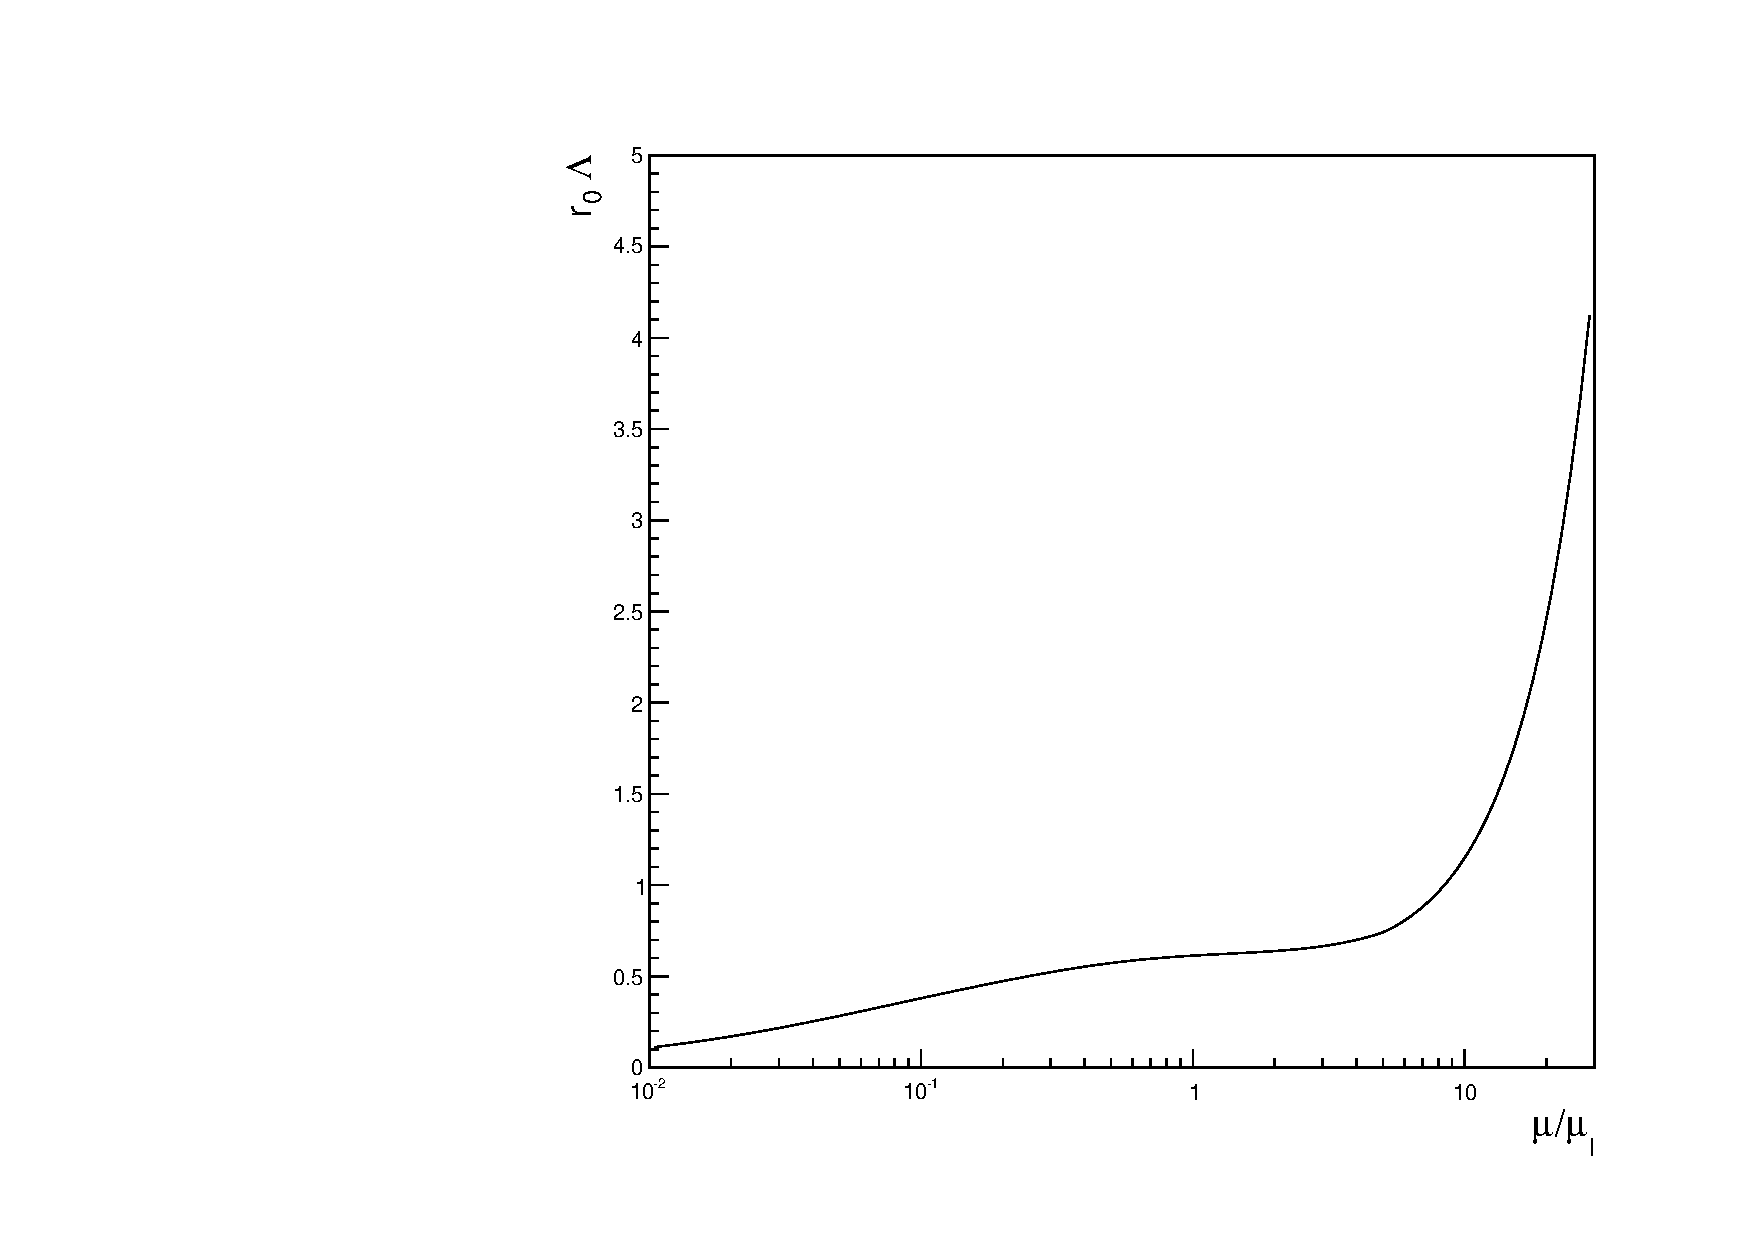
\includegraphics[width=3.5in]{method_I_stability.pdf}
  \caption{Stability analysis for the choice of scale in Method I for $n_f=0$ with the boosted coupling scheme.}
  \label{fig:method_I_stability}
\end{center}
\end{figure}

With respect to the chosen scale $\mu_\one^\boost$, the stability of the extrapolated value for $r_0 \Lambda_{(n_f)}^\msbar$ is important.
If $r_0 \Lambda_{(n_f)}^\msbar$ were to vary too much with small variations in the scale, the reliability of the method 
could be called into question. As a simple stability analysis, the continuum limit value for $r_0 \Lambda_{(0)}^\msbar$ is
plotted in Figure \ref{fig:method_I_stability} as a function of $\mu/\mu_\one^\boost$. It can be seen that the curve is flattest near the
scale $\mu = \mu_\one^\boost$, showing that $\mu_\one^\boost$ is, after all, a good choice for the scale. For details on the equations
used to find $r_0 \Lambda_{(n_f)}^\msbar (\mu/\mu_\one)$, see Appendix \ref{sec:stab_anal}. \vfill

\subsection{Method II} \label{sec:method_II} %%%%%%%%%%%%%%%%%%%%%%%%%%%%%%%%%

The motivation for this method is to eliminate \emph{all} the correction coefficients $d_n^\boost$ in eq. (\ref{eq:alpha_conversion}) 
for $n \ge 1$, effectively setting
\begin{equation} \label{eq:alpha_equivalence_II} \begin{aligned}
\alpha_\msbar(\mu_\two) = \alpha_\boost(a) .
\end{aligned} \end{equation}

For this to occur, the scale must be set to
\begin{equation} \label{eq:scale_choice_II} \begin{aligned}
\mu_\two^\boost = \frac{1}{a} \exp \paren{\frac{t_1^\boost}{2\beta_0}} \frac{M^\msbar(\alpha_\boost(a))}{M^\boost(\alpha_\boost(a))} .
\end{aligned} \end{equation}

To calculate the quantity $M^\boost(\alpha_\boost(a))$ to 3-loop order, the beta function coefficient $\beta_2^\boost$
must first be determined via eq. (\ref{eq:b2_relation}). Thereafter, this method gives 
\begin{equation} \label{eq:central_equation_II} \begin{aligned}
r_0 \Lambda_{(n_f)}^\msbar = \paren{ \frac{r_0}{a} } \exp{\paren{\frac{t_1^\boost}{2\beta_0}}} 
\frac{M^\msbar(\alpha_\boost(a))}{M^\boost(\alpha_\boost(a))M^\msbar(\alpha_\msbar(\mu_\two))} ,
\end{aligned} \end{equation}

\begin{figure}[h]
\begin{center}
  \vspace{-10pt}
  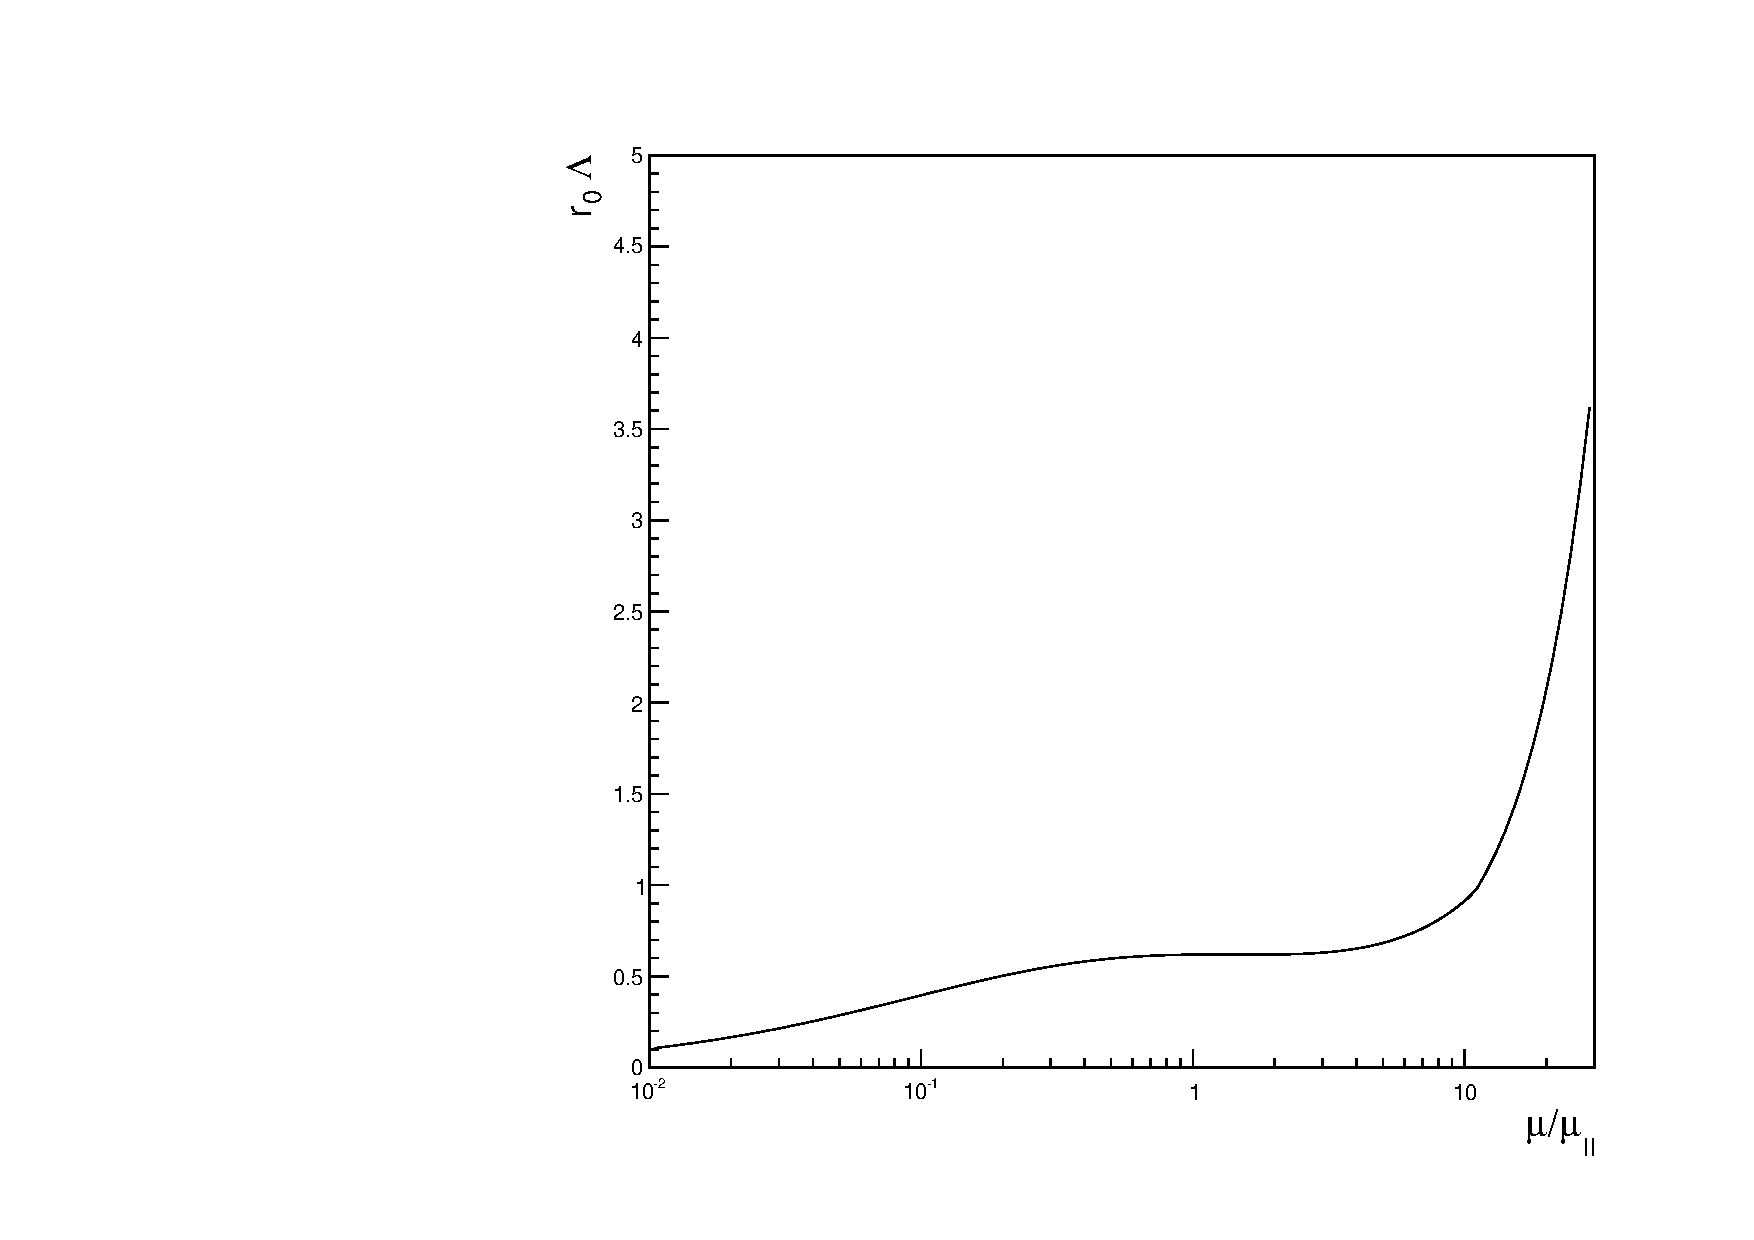
\includegraphics[width=3.5in]{method_II_stability.pdf}
  \caption{Stability analysis for the choice of scale in Method II for $n_f=0$. }
  \label{fig:method_II_stability}
\end{center}
\end{figure}

where $\alpha_\boost(a)$ must first be calculated using eq. (\ref{eq:boosted_coupling_def}). Of course, the factor 
$M^\msbar(\alpha_\boost(a))$ in the denominator cancels the $M^\msbar(\alpha_\msbar(a))$ factor in the numerator, but the chosen form 
is particularly well suited for conveying the details of the calculation, and is needed for the stability analysis of the resulting 
$r_0 \Lambda_{(0)}^\msbar$ shown in Figure \ref{fig:method_II_stability}.

Using the Pad\'{e} approximant method of \S\ref{sec:pade_approximants}, the beta function coefficient $\beta_3^\boost$ can be estimated,
allowing the function $M^\boost(\alpha_\boost(a))$ to be calculated to 4-loop order. When this estimation procedure is used, the method
is labelled as Method IIP. 

\vfill

\subsection{Method III}  \label{sec:method_III} %%%%%%%%%%%%%%%%%%%%%%%%%%%%%%%%%%

The philosophy of this method is to choose the scale in the same manner as in Method II, but to construct the boosted 
coefficients $b_i^\boost$, $d_j^\boost$, and $t_k^\boost$ in such a way that they are independent of the coupling 
$\alpha_\boost$. These variables only depend on the coupling through the $c_{sw}^\boost$ coefficient, so the strategy is to fix 
$c_{sw}^\boost$ to a constant value while maintaining both its perturbative consistency and its improvement properties. This
is done using the perturbative expansion 
\begin{equation} \label{eq:c_sw_perturb} \begin{aligned}
c_{sw}^\boost = 1 + c_0^\boost \alpha_\boost + \order{\alpha_\boost^2} ,
\end{aligned} \end{equation}

where $c_0^\boost = 0.1998$ \cite{Gockeler:2005}. To begin, eq. (\ref{eq:inverse_alpha_conversion}) is written in 
terms of $t_1^\boost$ and $t_2^\boost$ via eq. (\ref{eq:d_t_relations}), simplified by setting $a=1/\mu$, then is differentiated 
by $\partial / \partial \ln \mu^2$, leaving
\begin{equation} \label{eq:method_II_deriv_1} \begin{aligned}
\beta^\msbar(\alpha_\msbar) \frac{1}{\alpha_\msbar^2} = \beta^\boost(\alpha_\boost) 
\bracket{\frac{1}{\alpha_\boost^2}+\frac{\partial t_1^\boost}{\partial c_{sw}^\boost}\frac{\partial c_{sw}^\boost}{\partial \alpha_\boost} 
 + t_2^\boost+\order{\alpha_\boost}}  ,
\end{aligned} \end{equation}

where the definition of the beta function, eq. (\ref{eq:beta_def}), was used. Expanded out in powers of $\alpha_\boost$, it is found that
\begin{equation} \label{eq:b2_methodIII} \begin{aligned}
\beta_2^\boost &= \beta_2^\msbar + \beta_1 t_1^\boost |_{c_{sw}^\boost=1} - \beta_0 t_2^\boost|_{c_{sw}^\boost=1} 
- \beta_0 c_0^\boost \frac{\partial t_1^\boost}{\partial c_{sw}^\boost} |_{c_{sw}^\boost=1}  .
\end{aligned} \end{equation}

For this method, this is the equation used to calculate $\beta_2^\boost$, rather than eq. (\ref{eq:b2_relation}). The scale $\mu_\three$ 
is chosen in the same way as in Method II, but with $t_1^\boost$ evaluated at $c_{sw}^\boost=1$, leaving the following equation 
for calculating $r_0 \Lambda_{(n_f)}^\msbar$
\begin{equation} \label{eq:central_equation_III} \begin{aligned}
r_0 \Lambda_{(n_f)}^\msbar = \paren{ \frac{r_0}{a} } \exp{\paren{\frac{t_1^\boost |_{c_{sw}^\boost=1} }{2\beta_0}}} 
\frac{1}{M^\boost(\alpha_\boost(a))} ,
\end{aligned} \end{equation}

where again, $\alpha_\boost(a)$ must be calculated using eq. (\ref{eq:boosted_coupling_def}). As with Method II, there is an opportunity 
to use Pad\'{e} approximants to estimate the beta function coefficient $\beta_3^\boost$. When this estimation procedure is used, the 
method is labelled as Method IIIP.





\section{Crossing the Quark Thresholds} \label{sec:crossing_thresholds}

Since the data used in this paper is drawn only from $n_f=0$ and $n_f=2$ lattice simulations, the three methods provided in the 
previous section can only be used to calculate $\Lambda_{(0)}^\msbar$ and $\Lambda_{(2)}^\msbar$, though $\Lambda_{(5)}^\msbar$ is 
needed to finally determine $\alpha_\msbar^{(n_f=5)}(m_Z)$. The scale at which the $n_f=2$ effective theory no longer applies is 
at the mass of the strange quark; at scales above this threshold, the $n_f=3$ effective theory takes over. At this scale 
$\alpha_\msbar$ is large, precluding the use of a perturbative matching calculation between $\alpha_\msbar^{(3)}$ and $\alpha_\msbar^{(2)}$.
Instead, a matching procedure involving the $\Lambda_{(n_f)}^\msbar$ parameters is used. In contrast, the direct matching of 
$\alpha_\msbar^{(n_f+1)}$ to $\alpha_\msbar^{(n_f)}$ at the charm and beauty thresholds is done perturbatively, since at these
scales $\alpha_\msbar$ is small enough for the effective use of perturbative methods.

\subsection{Crossing the Strange Threshold} \label{sec:strange_threshold}

Two quarks held at a distance $r$ from one another experience a force analogous to the Coulomb force experienced by two static
electric charges. The static quark potential is known to 3-loop order \cite{Smirnov:2010} but only 2-loop results will be used here, since
the 3-loop correction is complicated by terms of the form $\alpha_\msbar^4 \ln \alpha_\msbar$. To 2-loop order, the static quark potential
is \cite{Peter:1997}
\begin{equation} \label{eq:static_potential_1_loop} \begin{aligned}
V(r;\alpha_\msbar^{(n_f)},\mu)=-\frac{4}{3}\frac{\alpha_\msbar^{(n_f)}}{r} \biggl\{ 1&+\alpha_\msbar^{(n_f)}\bracket{2\beta_0 \ln (\mu r') + a_1}  \biggr. \\
&+ (\alpha_\msbar^{(n_f)})^2 \biggl[ \beta_0^2\paren{4\ln^2(\mu r')+\frac{\pi^2}{3}} \biggr.  \\
&\ \ \ \ \ \ \ \ \ \ \biggl. \biggl. + 2(\beta_1+2\beta_0 a_1)\ln(\mu r') + a_2  \biggr] + \order{\alpha_\msbar^3} \biggr\} ,
\end{aligned} \end{equation}

where $r' \equiv re^\gamma$ and the two constant $a_1$ and $a_2$ are \cite{Schroder:1998,Schroder:1999}
\begin{equation} \label{eq:static_potential_a1a2} \begin{aligned}
a_1 &= \frac{1}{4\pi}\bracket{ \frac{31}{3} - \frac{10}{9}n_f  }\\
a_2 &= \frac{1}{(4\pi)^2} \bracket{ \paren{\frac{4343}{18}+36\pi^2 - \frac{9\pi^4}{4} + 66\zeta_3}
      - \paren{\frac{1229}{27} +\frac{52}{3}\zeta_3}n_f + \frac{100}{81}n_f^2 } .
\end{aligned} \end{equation}

The force experienced by a second quark at a distance $r$ from the first is calculated from\footnote{Note the opposite sign convention.} 
$f(r)=dV/dr$, leading to the expression 

\begin{equation} \label{eq:static_force} \begin{aligned}
r^2 f(r)=\frac{4}{3}\alpha_\msbar \biggl\{ 1&+\alpha_\msbar \bracket{2\beta_0 \ln (\mu r') + a_1 -2\beta_0}      \biggr. \\
& + \alpha_\msbar^2 \biggl[ \beta_0^2\paren{4 \ln^2 (\mu r') - 8 \ln (\mu r') + \frac{\pi^2}{3} } \biggr. \\
& \ \ \ \ \ \ \ \ \ \ \ \ \ \ \ \ \ \ \biggl. \biggl. + 2(\beta_1+2\beta_0 a_1)(\ln (\mu r') -1) + a_2 \biggr] + \order{\alpha_\msbar^3} \biggr\}  .
\end{aligned} \end{equation}

Defining a force-scale coupling $\alpha_\qqbar$ by \cite{Necco:2001}
\begin{equation} \label{eq:static_force_qqbar} \begin{aligned}
r^2 f(r) = \frac{4}{3} \alpha_\qqbar (r)  ,
\end{aligned} \end{equation}

the expansion coefficients $d_1^\qqbar$ and $d_2^\qqbar$ for the conversion from the force-scale coupling scheme to the $\overline{MS}$ 
can be shown to be
\begin{equation} \label{eq:d1d2_qqbar} \begin{aligned}
d_1^\qqbar &= 2 \beta_0 - a_1 - 2\beta_0 \ln (\mu r')  \\
d_2^\qqbar &= (d_1^\qqbar)^2 - 2 \beta_1 \ln (\mu r') + \beta_0^2\paren{4-\frac{\pi^2}{3}} +2\beta_1(1-\gamma) + a_1^2 - a_2  ,
\end{aligned} \end{equation}

which gives the conversion variables $t_1^\qqbar$ and $t_2^\qqbar$ as
\begin{equation} \label{eq:t1t2_qqbar} \begin{aligned}
t_1^\qqbar &= 2 \beta_0(1-\gamma) - a_1   \\
t_2^\qqbar &= \beta_0^2\paren{4-\frac{\pi^2}{3}} +2\beta_1(1-\gamma) + a_1^2 - a_2  .
\end{aligned} \end{equation}

Assuming now that the force $f(r^*)$ between static quarks is $n_f$-independent at some particular distance $r^*$, then 
from eq. (\ref{eq:static_force_qqbar}) so too is $\alpha_\qqbar(r^*)$. From eqs. (\ref{eq:beta_integ_NLloop}) and (\ref{eq:M_of_alpha}),
the relation
\begin{equation} \label{eq:rstar_usage} \begin{aligned}
r^* \Lambda_{(n_f)}^\qqbar = \frac{1}{M_{(n_f)}^\qqbar(\alpha_\qqbar)}
\end{aligned} \end{equation}

can be used to calculate ratios of $\Lambda^\qqbar$ that are independent of the $r^*$. Equation (\ref{eq:t1_def}) then converts these
ratios of $\Lambda^\qqbar$ into ratios of $\Lambda^\msbar$. Concretely, the ratios
\begin{equation} \label{eq:lambda_ratios20} \begin{aligned}
\frac{\Lambda_{(2)}^\msbar}{\Lambda_{(0)}^\msbar} = \frac{\exp \paren{\frac{t_{1(2)}^\qqbar}{2\beta_0^{(2)}}} M_{(0)}^\qqbar(\alpha_\qqbar)}{\exp \paren{\frac{t_{1(0)}^\qqbar}{2\beta_0^{(0)}}} M_{(2)}^\qqbar(\alpha_\qqbar)}
\end{aligned} \end{equation}

and
\begin{equation} \label{eq:lambda_ratios32} \begin{aligned}
\frac{\Lambda_{(3)}^\msbar}{\Lambda_{(2)}^\msbar} = \frac{\exp \paren{\frac{t_{1(3)}^\qqbar}{2\beta_0^{(3)}}} M_{(2)}^\qqbar(\alpha_\qqbar)}{\exp \paren{\frac{t_{1(2)}^\qqbar}{2\beta_0^{(2)}}} M_{(3)}^\qqbar(\alpha_\qqbar)}
\end{aligned} \end{equation}

can be determined as functions of $\alpha_\qqbar$. By choosing an arbitrary value of $\Lambda_{(2)}^\msbar / \Lambda_{(0)}^\msbar$,
eq. (\ref{eq:lambda_ratios20}) can be numerically inverted to give the corresponding value of $\alpha_\qqbar$. Inputting
this output into eq. (\ref{eq:lambda_ratios32}) thus gives $\Lambda_{(3)}^\msbar / \Lambda_{(2)}^\msbar$ as a function
of $\Lambda_{(2)}^\msbar / \Lambda_{(0)}^\msbar$. This is shown in Figure \ref{fig:rat32_v_rat20_bad}. 

\begin{figure}[h]
\begin{center}
  \vspace{-10pt}
  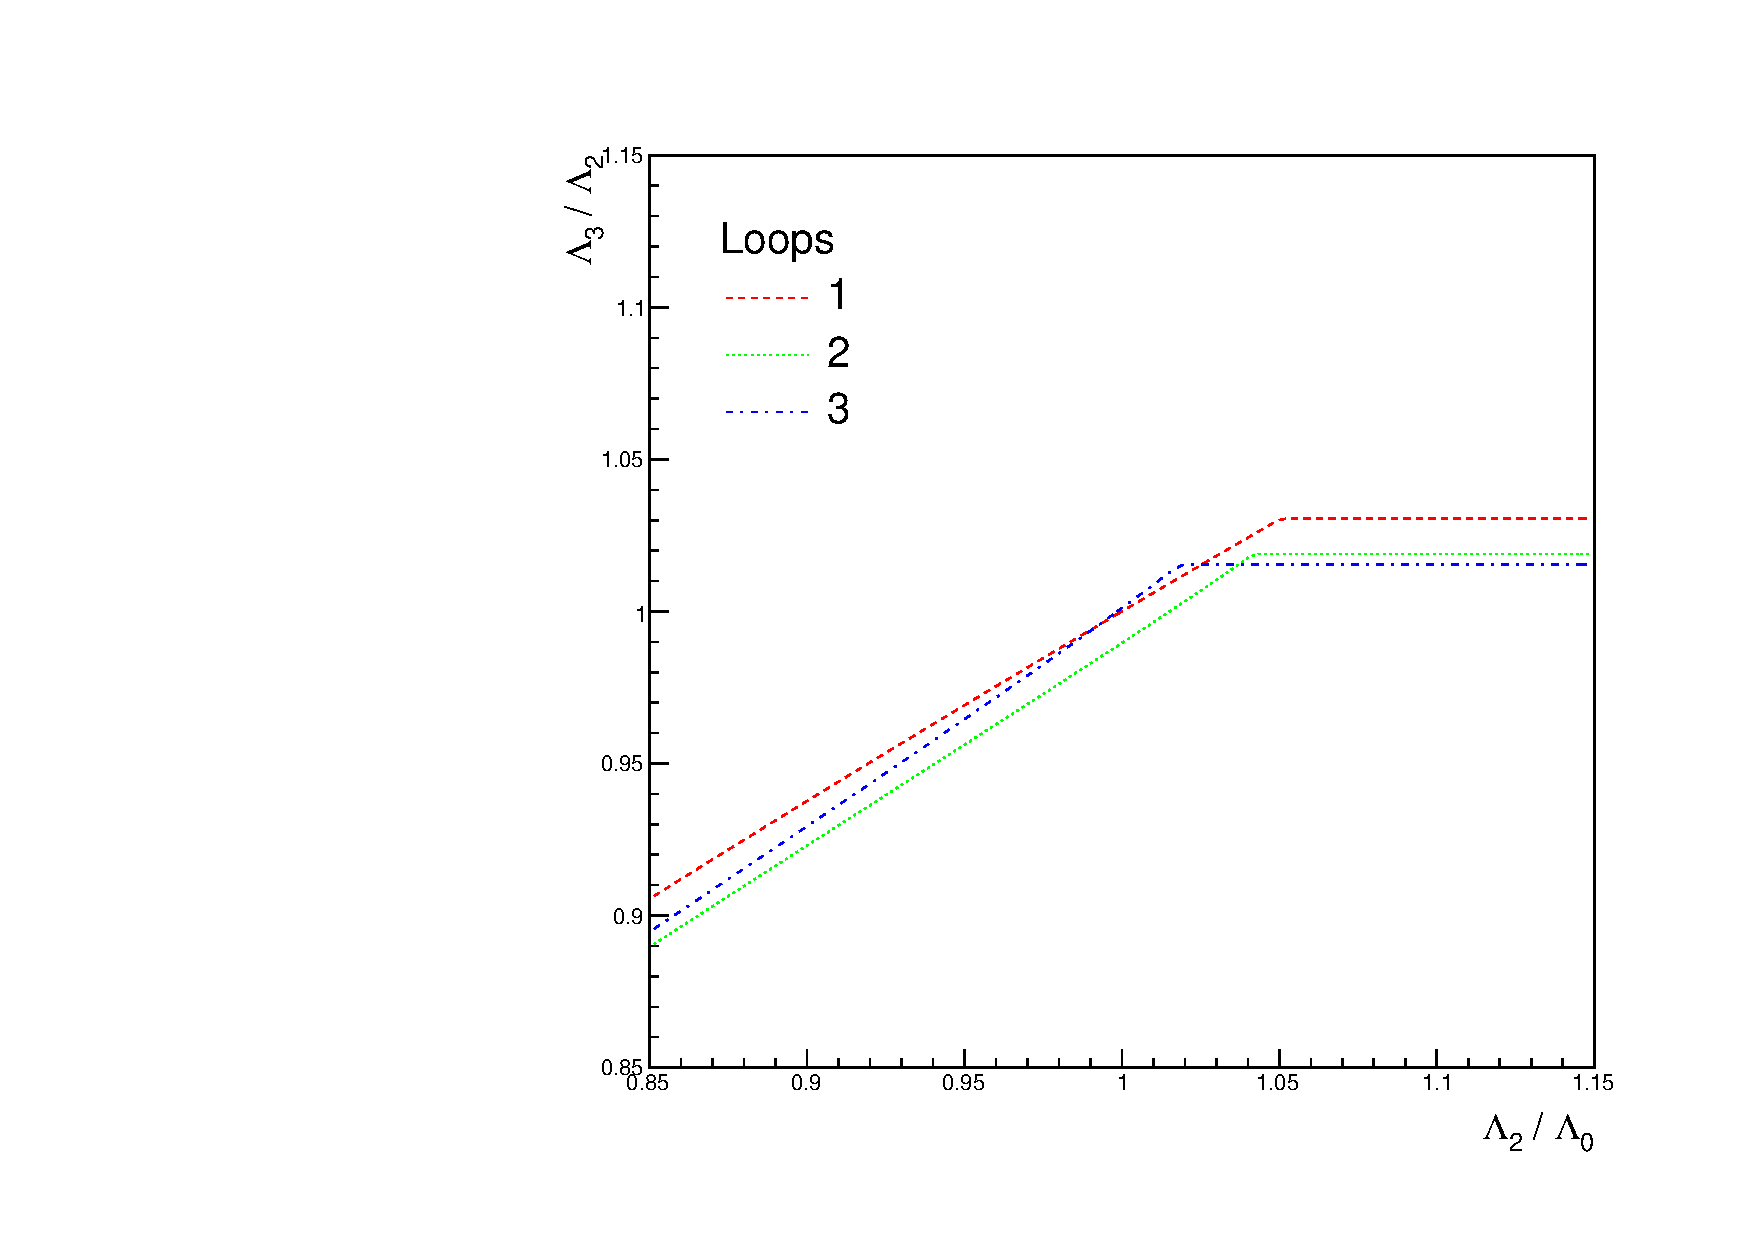
\includegraphics[width=3.5in]{rat32_v_rat20_bad.pdf}
  \caption{$\Lambda_{(3)}^\msbar / \Lambda_{(2)}^\msbar$ versus $\Lambda_{(2)}^\msbar / \Lambda_{(0)}^\msbar$. }
  \label{fig:rat32_v_rat20_bad}
  \vspace{-10pt}
\end{center}
\end{figure}

Looking at Figure \ref{fig:rat32_v_rat20_bad}, something is quite clearly going wrong at 
$\Lambda_{(2)}^\msbar / \Lambda_{(0)}^\msbar \sim 1.05$:
the smooth curves abruptly become perfectly horizontal. What this represents is the fact that as 
$\alpha_\qqbar \rightarrow \infty$, $\Lambda_{(2)}^\msbar / \Lambda_{(0)}^\msbar$ reaches its asymptotic value of $\sim1.05$. 
When the numerical inversion algorithm can't find a value for $\alpha_\qqbar$ that corresponds to a large ($>1.05$) value of
$\Lambda_{(2)}^\msbar / \Lambda_{(0)}^\msbar$, it outputs the highest value of $\alpha_\qqbar$ that it is allowed to give.
This highest value is then used as input to calculate $\Lambda_{(3)}^\msbar / \Lambda_{(2)}^\msbar$, producing the 
horizontal line lying at a y-value equal to the asymptotic value of $\Lambda_{(3)}^\msbar / \Lambda_{(2)}^\msbar$.
This would be fine so long as $\Lambda_{(2)}^\msbar / \Lambda_{(0)}^\msbar \lesssim 1.05$, as was found in \cite{Gockeler:2005}, where this 
matching procedure was used with great success. Unfortunately, the results in Chapter \ref{sec:data_and_results} show 
$\Lambda_{(2)}^\msbar / \Lambda_{(0)}^\msbar > 1.05$. This is clearly a problem.

To save this method, recall that in the region $\Lambda_{(2)}^\msbar / \Lambda_{(0)}^\msbar \sim 1.05$, the expansion parameter
$\alpha_\qqbar$ is large. This means that the abrupt cutoff to a horizontal line in Figure \ref{fig:rat32_v_rat20_bad} is just
a symptom of perturbation theory breaking down. Consequently, any attempt to predictively use $\alpha_\qqbar$ in this region
should be discouraged. Before this non-perturbative region is reached, however, it is observed that the curves are well-behaved
and slowly varying. With no reference to $\alpha_\qqbar$ anywhere in Figure \ref{fig:rat32_v_rat20_bad}, there is no
reason to expect this behaviour to change in the region $\Lambda_{(2)}^\msbar / \Lambda_{(0)}^\msbar > 1.05$. This allows
a Taylor series to be constructed, fitting the curves in the the perturbative region and extrapolating to the non-perturbative region.

\begin{figure}[h!]
\begin{center}
  \vspace{-10pt}
  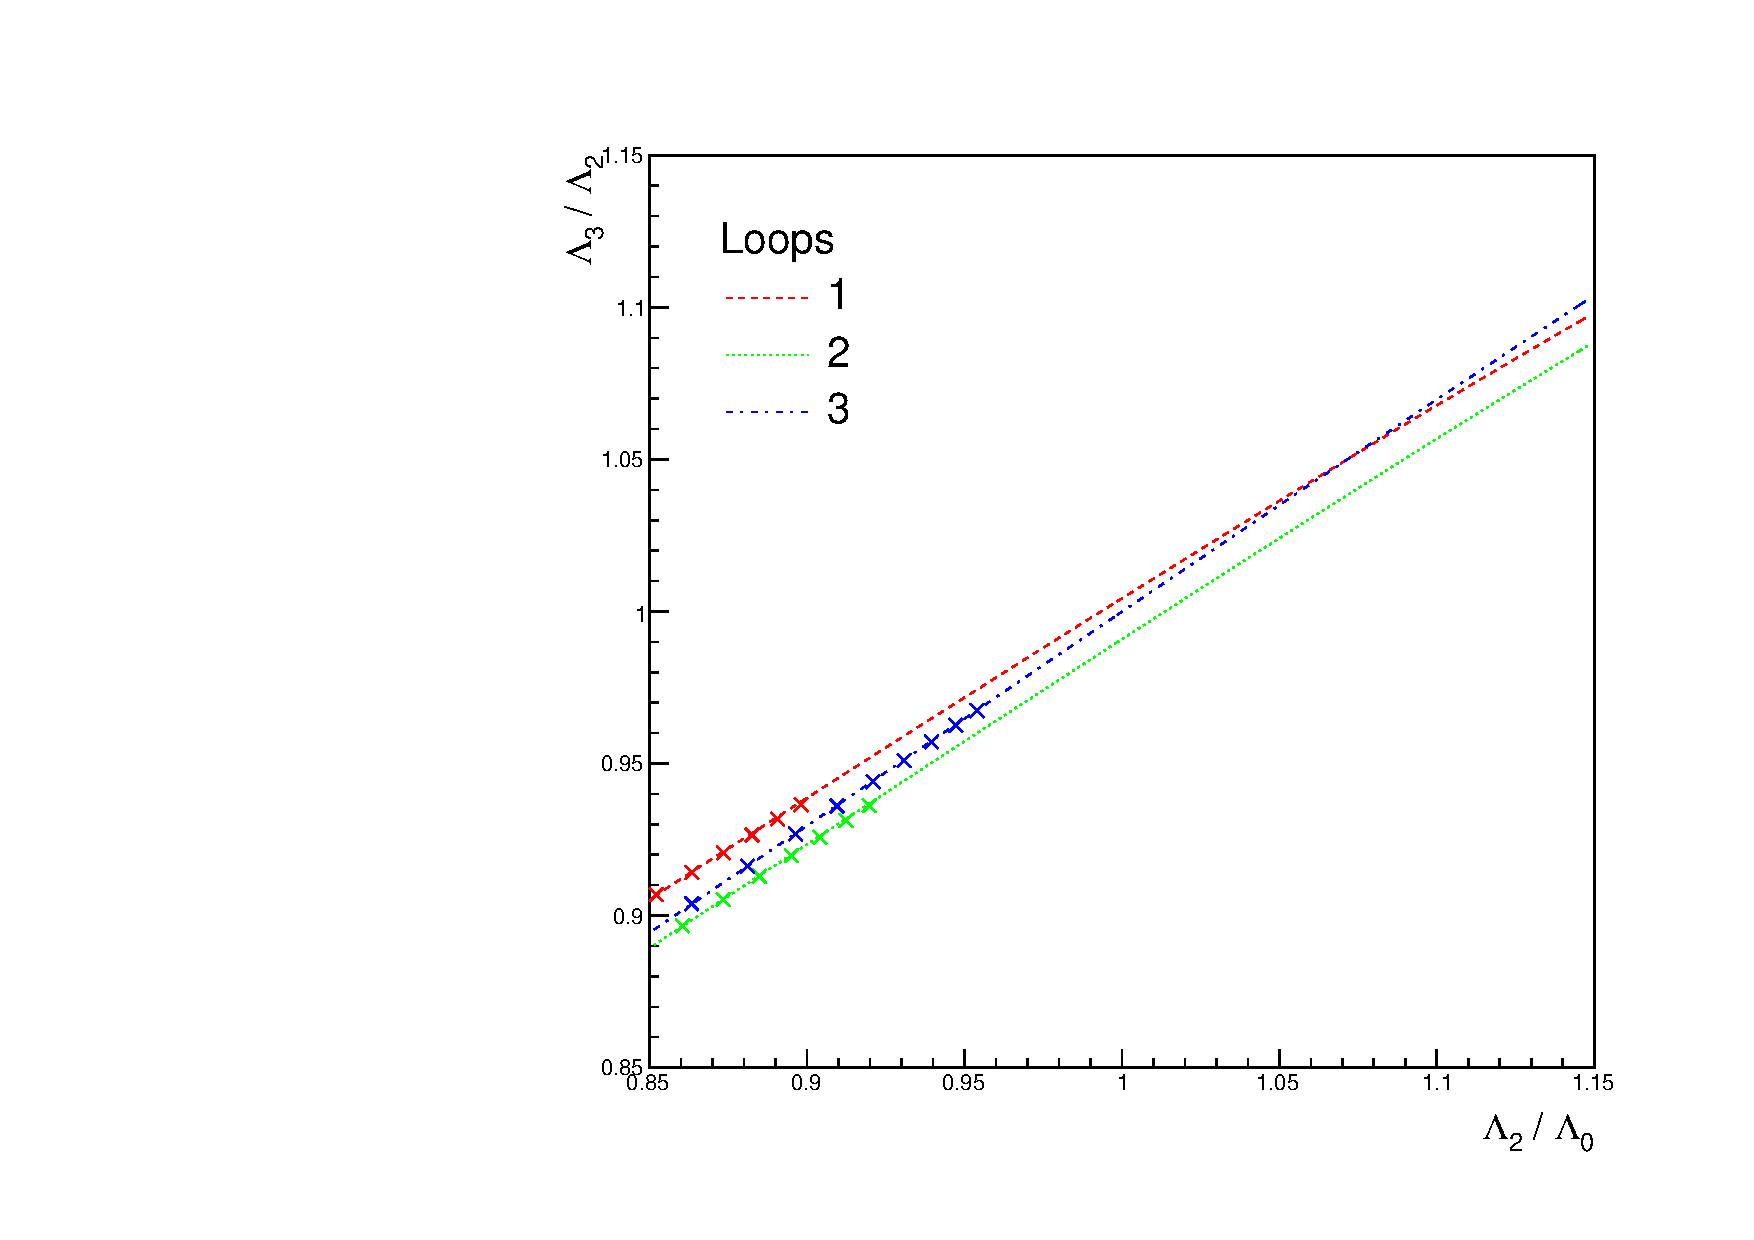
\includegraphics[width=3.5in]{rat32_v_rat20_good.pdf}
  \caption{Fitted and extrapolated $\Lambda_{(3)}^\msbar / \Lambda_{(2)}^\msbar$ versus $\Lambda_{(2)}^\msbar / \Lambda_{(0)}^\msbar$ 
curves using a quartic series expansion about $\Lambda_{(2)}^\msbar / \Lambda_{(0)}^\msbar=1.1$. The X markers denote the points
which are used to fit the curves.}
  \label{fig:rat32_v_rat20_good}
  \vspace{-10pt}
\end{center}
\end{figure}

Believing that the region $\alpha_\qqbar < 0.5$ should give reliable perturbative results, 20 values of 
$\Lambda_{(2)}^\msbar / \Lambda_{(0)}^\msbar$ and $\Lambda_{(3)}^\msbar / \Lambda_{(2)}^\msbar$ are directly calculated with eqs. 
(\ref{eq:lambda_ratios20}) and (\ref{eq:lambda_ratios32}) for $0.025 \le \alpha_\qqbar \le 0.475$. These pairs are fitted with a quartic
polynomial in $\Lambda_{(2)}^\msbar / \Lambda_{(0)}^\msbar$, and expanded about $\Lambda_{(2)}^\msbar / \Lambda_{(0)}^\msbar = 1.1$, where
the expansion point was chosen from the results of Chapter \ref{sec:data_and_results}. The extrapolated curves are shown in Figure 
\ref{fig:rat32_v_rat20_good}. 

\subsection{Crossing the Charm and Beauty Thresholds} \label{sec:charm_beauty_thresholds}

At high enough energy scales, matching across quark thresholds can be done perturbatively. The matching condition reads \cite{Chetyrkin:1997}
\begin{equation} \label{eq:3_loop_matching} \begin{aligned}
\alpha_\msbar^{(n_f+1)} (m_q^\msbar\!)=\frac{1}{\zeta_g^2} \alpha_\msbar^{(n_f)} (m_q^\msbar\!)  ,
\end{aligned} \end{equation}

where $m_q^\msbar$ is the mass of the heavy quark evaluated at the scale $\mu = m_s^\msbar$. The prefactor is \cite{Chetyrkin:2000}
\begin{equation} \label{eq:inverse_zeta_squared} \begin{aligned}
\frac{1}{\zeta_g^2} = 1 - \frac{11}{72} \paren{ \frac{ \alpha_\msbar^{(n_f)}(m_q^\msbar\!) }{\pi} }^2 
+ \paren{ \frac{ \alpha_\msbar^{(n_f)}(m_q^\msbar\!) }{\pi} }^2 \paren{-\frac{564731}{124416} + \frac{82043}{27648}\zeta_3 + \frac{2633}{31104}n_f }.
\end{aligned} \end{equation}

Thus once the parameter $\Lambda_{(3)}^\msbar$ is determined the process is as follows: $\alpha_\msbar^{(n_f=3)}(m_c^\msbar\!)$ is 
determined by inverting eq. (\ref{eq:beta_integ_NLloop}), then $\alpha_\msbar^{(n_f=4)}(m_c^\msbar\!)$ is determined by matching 
across the charm threshold with eq. (\ref{eq:3_loop_matching}), and $\Lambda_{(4)}^\msbar$ is then found by once again using 
eq. (\ref{eq:beta_integ_NLloop}). This process is repeated to cross the bottom threshold, leading to a determination 
of $\Lambda_{(4)}^\msbar$. Finally, eq. (\ref{eq:beta_integ_NLloop}) is inverted again to find $\alpha_\msbar^{(n_f=5)}(m_Z)$. 

The Z boson mass and $\overline{MS}$ quark masses are drawn from the PDG review \cite{PDG}. The values used are 
\begin{equation} \label{eq:z_quark_masses} \begin{aligned}
m_Z=91.1876(21) && ; && m_c^\msbar(m_c^\msbar\!)=1.275(25) && ; && m_b^\msbar(m_b^\msbar\!)=4.18(3) .
\end{aligned} \end{equation}























\chapter{Data, Analysis, and Results} \label{sec:data_and_results}

This chapter pulls together the methods of \S\ref{sec:three_methods} to calculate $r_0 \Lambda_{(0)}^\msbar$ 
and $r_0 \Lambda_{(2)}^\msbar$. Equipped with these values, the methods of \S\ref{sec:crossing_thresholds} are used
to cross the strange, charm, and beauty thresholds, finally determining $\alpha_\msbar^{(n_f=5)}(m_Z)$.


\section{$n_f=0$} \label{sec:nf0}

The quenched data for $\beta$, $r_0/a$, and $P$ shown in Table \ref{tab:quenched_data} is taken directly from \cite{Gockeler:2005}. The
$r_0\Lambda_{(0)}^\msbar$ I$_\bare$ values come from Method I in the bare lattice scheme, the $r_0\Lambda_{(0)}^\msbar$ I$_\boost$ values
are found using Method I in the boosted coupling scheme, and the $r_0\Lambda_{(0)}^\msbar$ II and $r_0\Lambda_{(0)}^\msbar$ IIP values
are calculated using Method II in the boosted coupling scheme without and with the Pad\'{e} approximant estimations of $\beta_3^\boost$, 
respectively. Method III and IIIP values are not shown because in the quenched approximation there are no fermions on the lattice, so 
$c_{sw}^\boost=0$. This takes away the only difference between Method II and Method III, and
\begin{table}[h]
\begin{center}
\begin{tabular}{c c c c c c c }
\hline 
\rule{0pt}{3ex}    
$\beta$ & $r_0/a$ & $P$ & $r_0\Lambda_{(0)}^\msbar$ I$_\bare$ & $r_0\Lambda_{(0)}^\msbar$ I$_\boost$ & $r_0\Lambda_{(0)}^\msbar$ II  & $r_0\Lambda_{(0)}^\msbar$ IIP \\
\hline \hline
 5.70$^\dag$ & 2.922(09)         & 0.549195(25) & 0.3309(10) & 0.4849(15) & 0.4950(15) & 0.4877(15) \\
 5.80$^\dag$ & 3.673(05)         & 0.567651(21) & 0.3708(05) & 0.5106(07) & 0.5200(07) & 0.5130(07) \\
 5.95 & 4.898(12)         & 0.588066(20) & 0.4161(10) & 0.5429(13) & 0.5514(14) & 0.5448(13) \\
 6.00 & 5.368(33)         & 0.593679(08) & 0.4306(26) & 0.5548(34) & 0.5631(35) & 0.5566(34) \\
 6.07 & 6.033(17)         & 0.601099(18) & 0.4464(13) & 0.5666(16) & 0.5746(16) & 0.5683(16) \\
 6.20 & 7.380(26)         & 0.613633(02) & 0.4702(17) & 0.5833(21) & 0.5907(21) & 0.5847(21) \\
 6.40 & 9.740(50)         & 0.630633(04) & 0.4929(25) & 0.5953(31) & 0.6018(31) & 0.5963(31) \\
 6.57 & 12.18(10)\ \ \ \  & 0.643524(15) & 0.5066(42) & 0.6010(49) & 0.6069(50) & 0.6018(49) \\
 6.69 & 14.20(12)\ \ \ \  & 0.651936(15) & 0.5143(43) & 0.6035(51) & 0.6090(51) & 0.6042(51) \\
 6.81 & 16.54(12)\ \ \ \  & 0.659877(13) & 0.5216(38) & 0.6062(44) & 0.6113(44) & 0.6068(44) \\
 6.92 & 19.13(15)\ \ \ \  & 0.666721(12) & 0.5313(42) & 0.6128(48) & 0.6177(48) & 0.6133(48) \\  \rule{0pt}{2.5ex}    
 $\infty$ & $\infty$      & 1            & 0.5351(26) & 0.6138(19) & 0.6194(19) & 0.6145(19) \\
\hline
\end{tabular}
\end{center}
\caption{Plaquette and $r_0/a$ data for $n_f=0$, with corresponding $r_0\Lambda_{(0)}^\msbar$ values determined using the 4 methods.
 The last row represents extrapolated values in the continuum limit. Rows containing $\beta$-values marked with a `\dag' are not used in the fit.}
\label{tab:quenched_data}
\end{table}

thus the Method III values for $r_0\Lambda_{(0)}^\msbar$ are the same as in Method II.

The lattice simulations use the $\order{a}$-improved clover action, so it is expected that the leading order discretization effects should
behave like $a^2$. This motivates the extrapolation to the continuum limit with the independent variable being quadratic in the lattice 
spacing. However, as first discussed in \S\ref{sec:method_I}, Figure \ref{fig:methodI_bare} shows that the extrapolation to the continuum 
limit for $r_0\Lambda_{(0)}^\msbar$ is nonlinear in the squared lattice spacing $(a/r_0)^2$ when using the bare lattice scheme. This 
implies that the discretization errors are not fully controlled in the bare lattice scheme, and that the bare lattice scheme should 
be abandoned in favour of a scheme that has better control over the discretization effects. 

\begin{figure}[ht]
\begin{center}
  \subfloat[Method I$_\bare$ \label{fig:methodI_bare}]{
    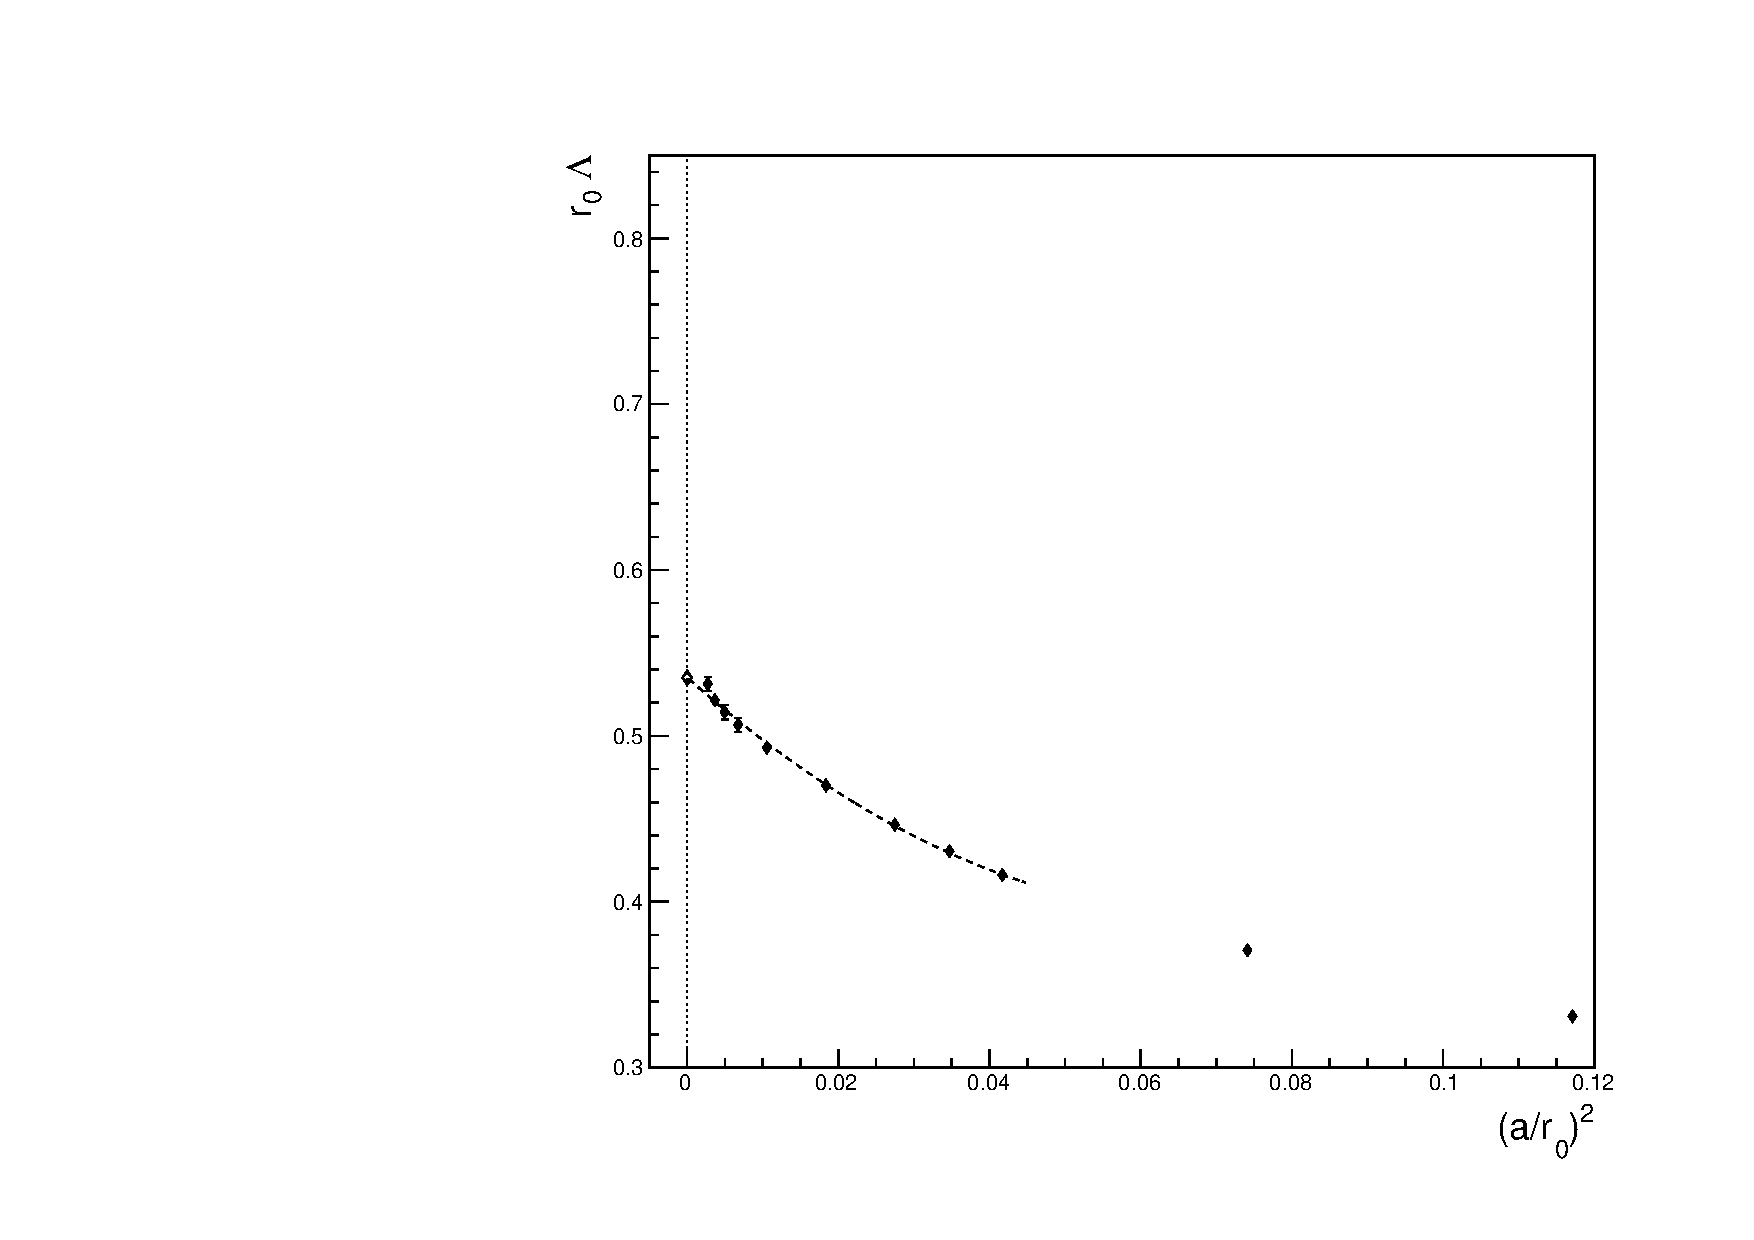
\includegraphics[width=0.50\textwidth]{methodI_lat_quenched.pdf}
  }
  \hspace{-0.27in}
  \subfloat[Method I$_\boost$ \label{fig:methodI_boosted}]{
    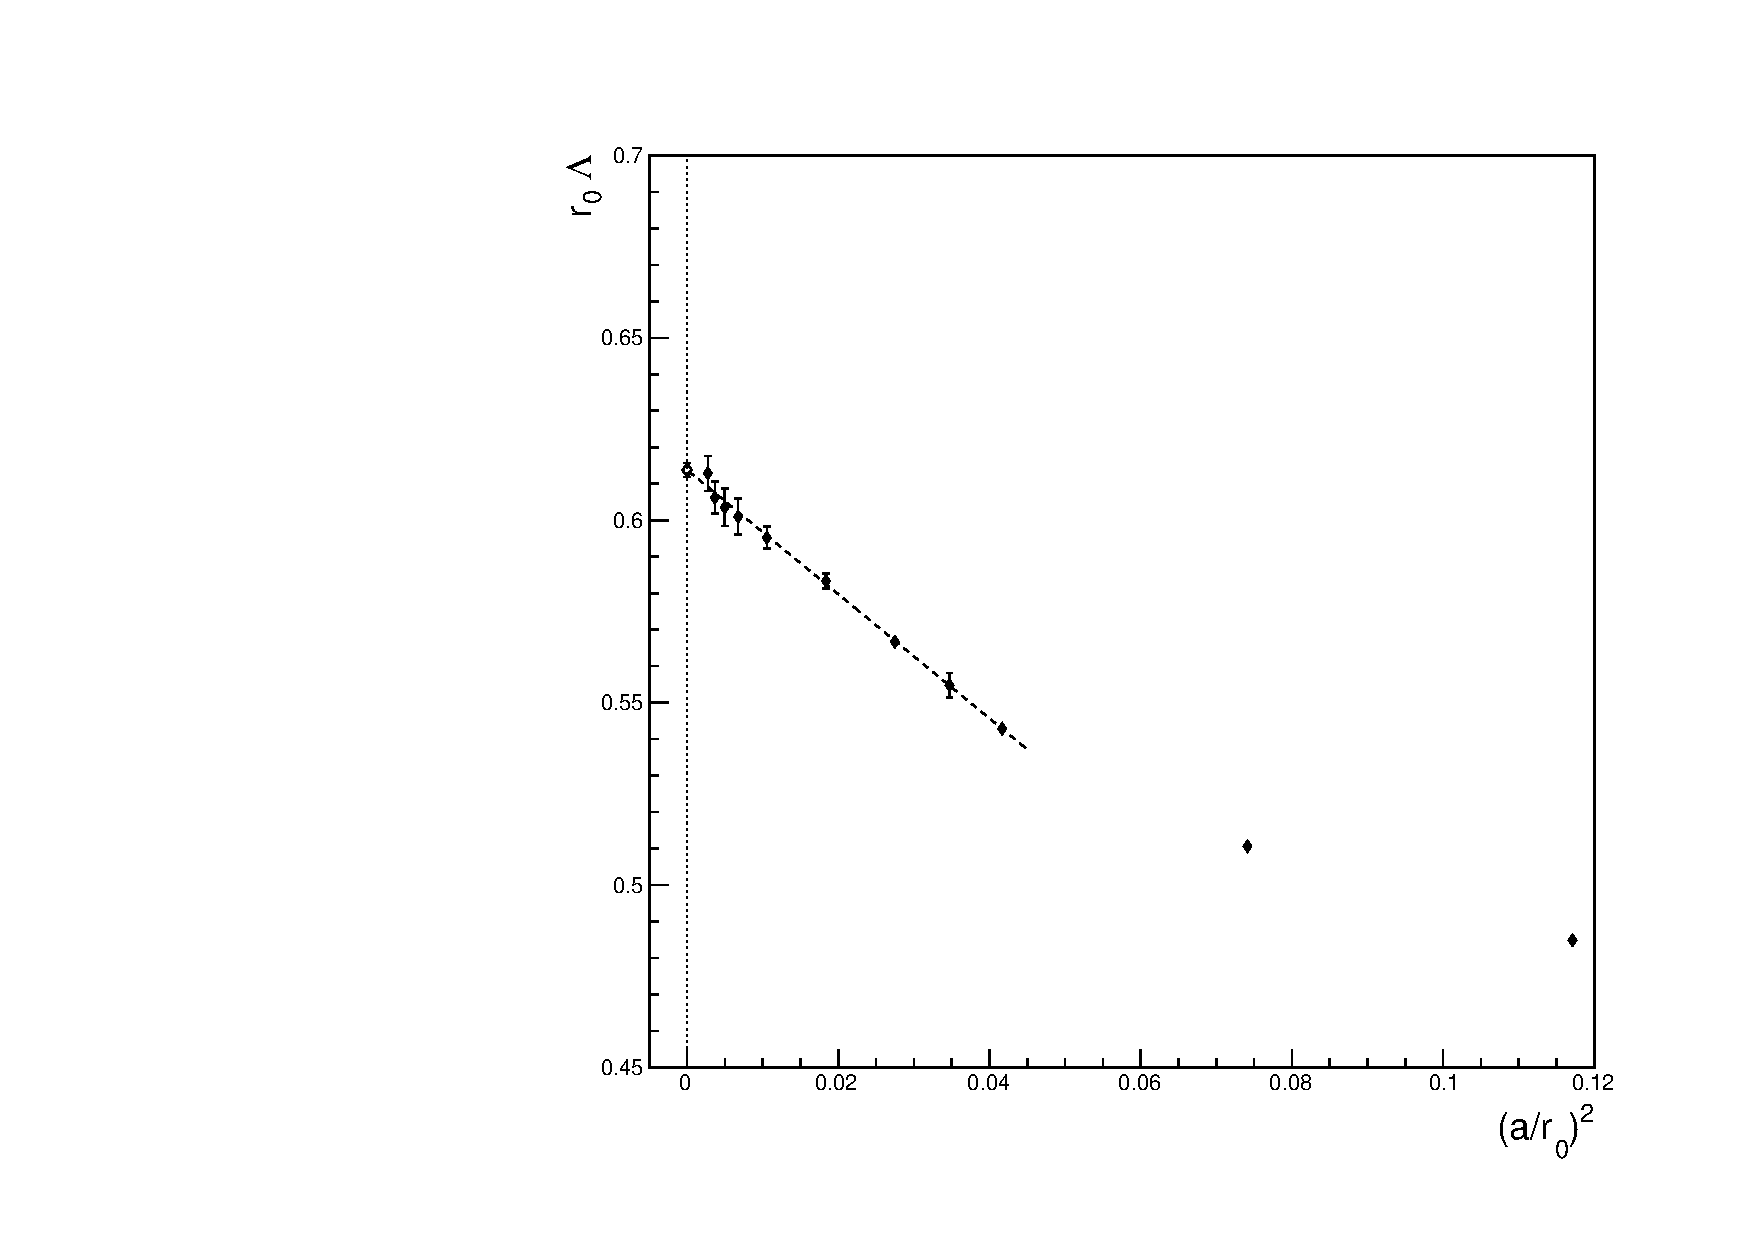
\includegraphics[width=0.50\textwidth]{methodIquenched.pdf}
  }
  \caption{Extrapolation of $r_0\Lambda_{(0)}^\msbar$ to the continuum limit in the quenched approximation for Method I using the 
bare lattice scheme (left) and the boosted coupling scheme (right).}
  \label{fig:methodI_bare_boost}
\end{center}
\end{figure}

\begin{figure}[h!]
\begin{center}
  \subfloat[Method II \label{fig:method_II_quenched}]{
    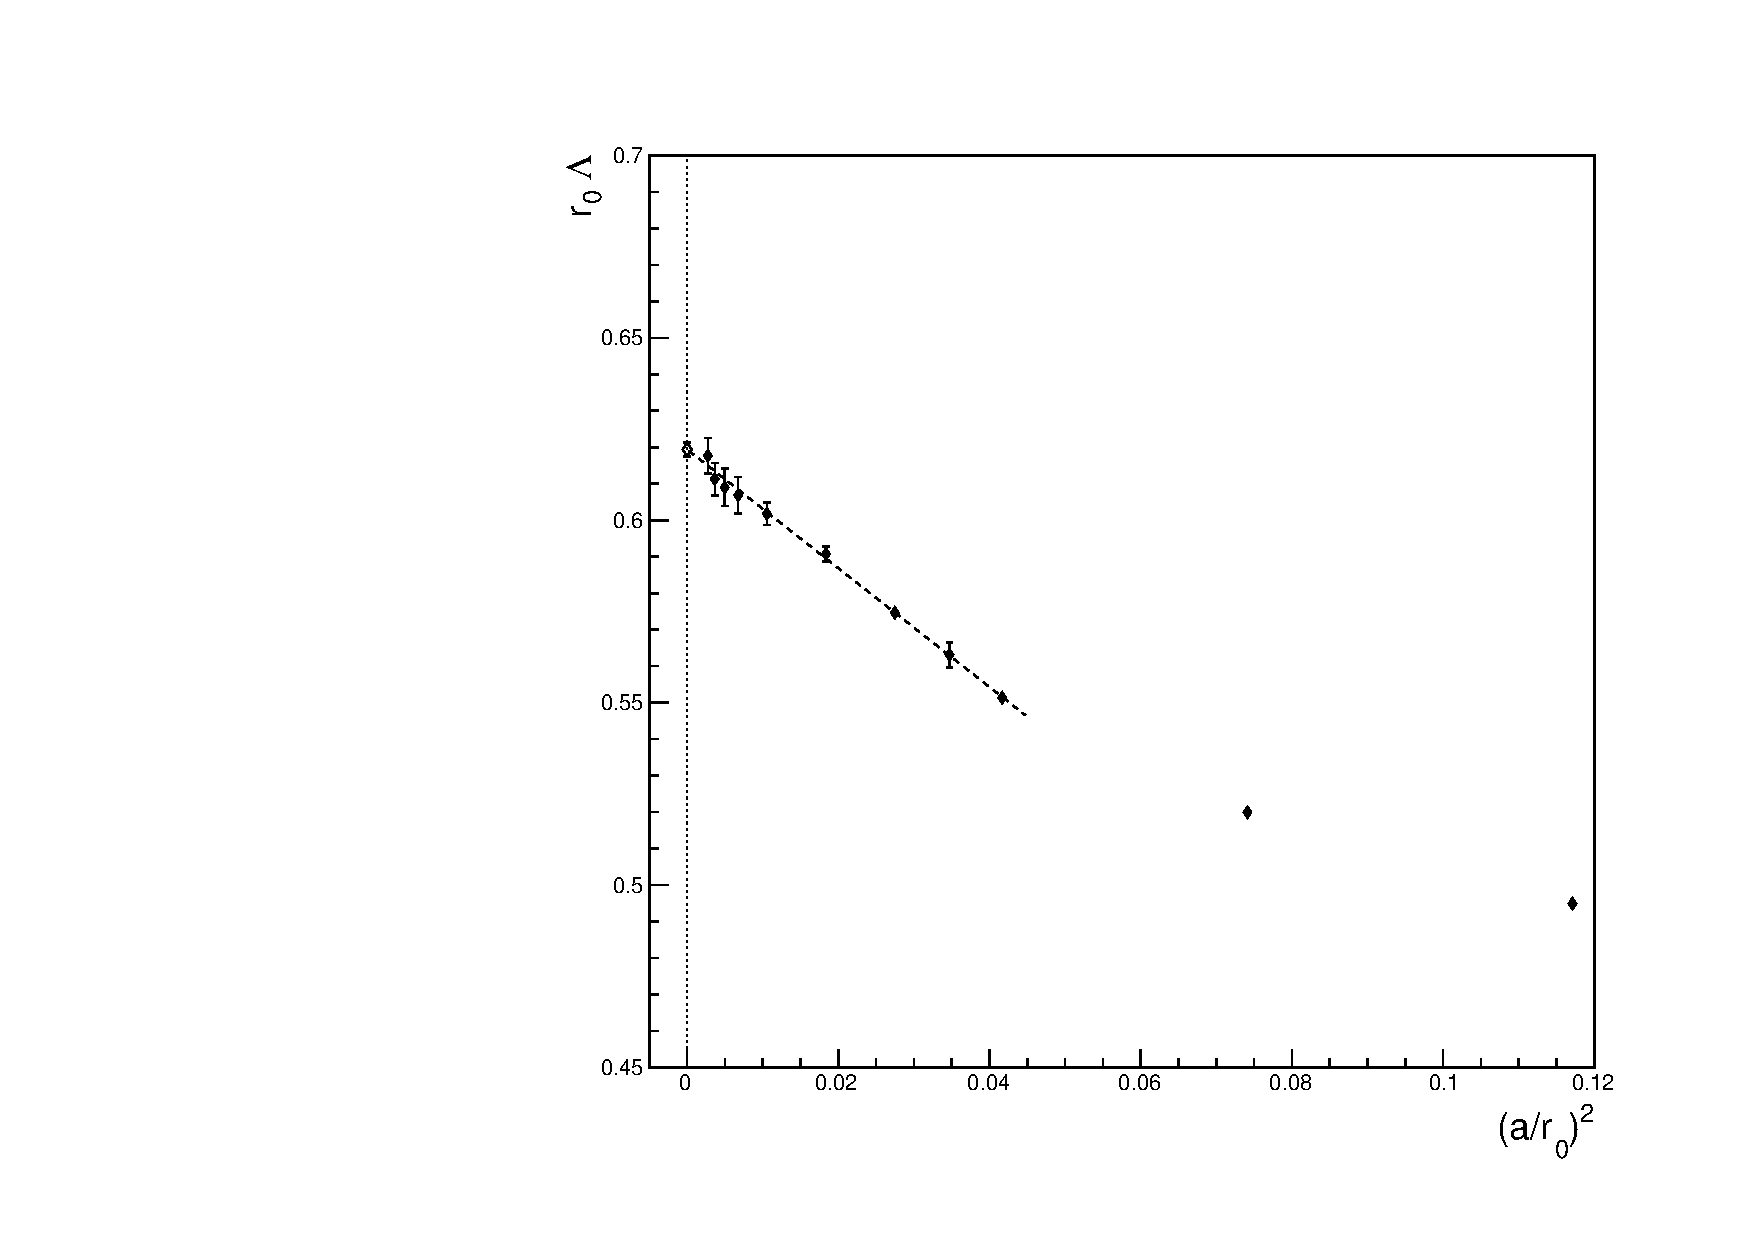
\includegraphics[width=0.50\textwidth]{methodIIquenched.pdf}
  }
  \hspace{-0.27in}
  \subfloat[Method IIP \label{fig:method_IIP_quenched}]{
    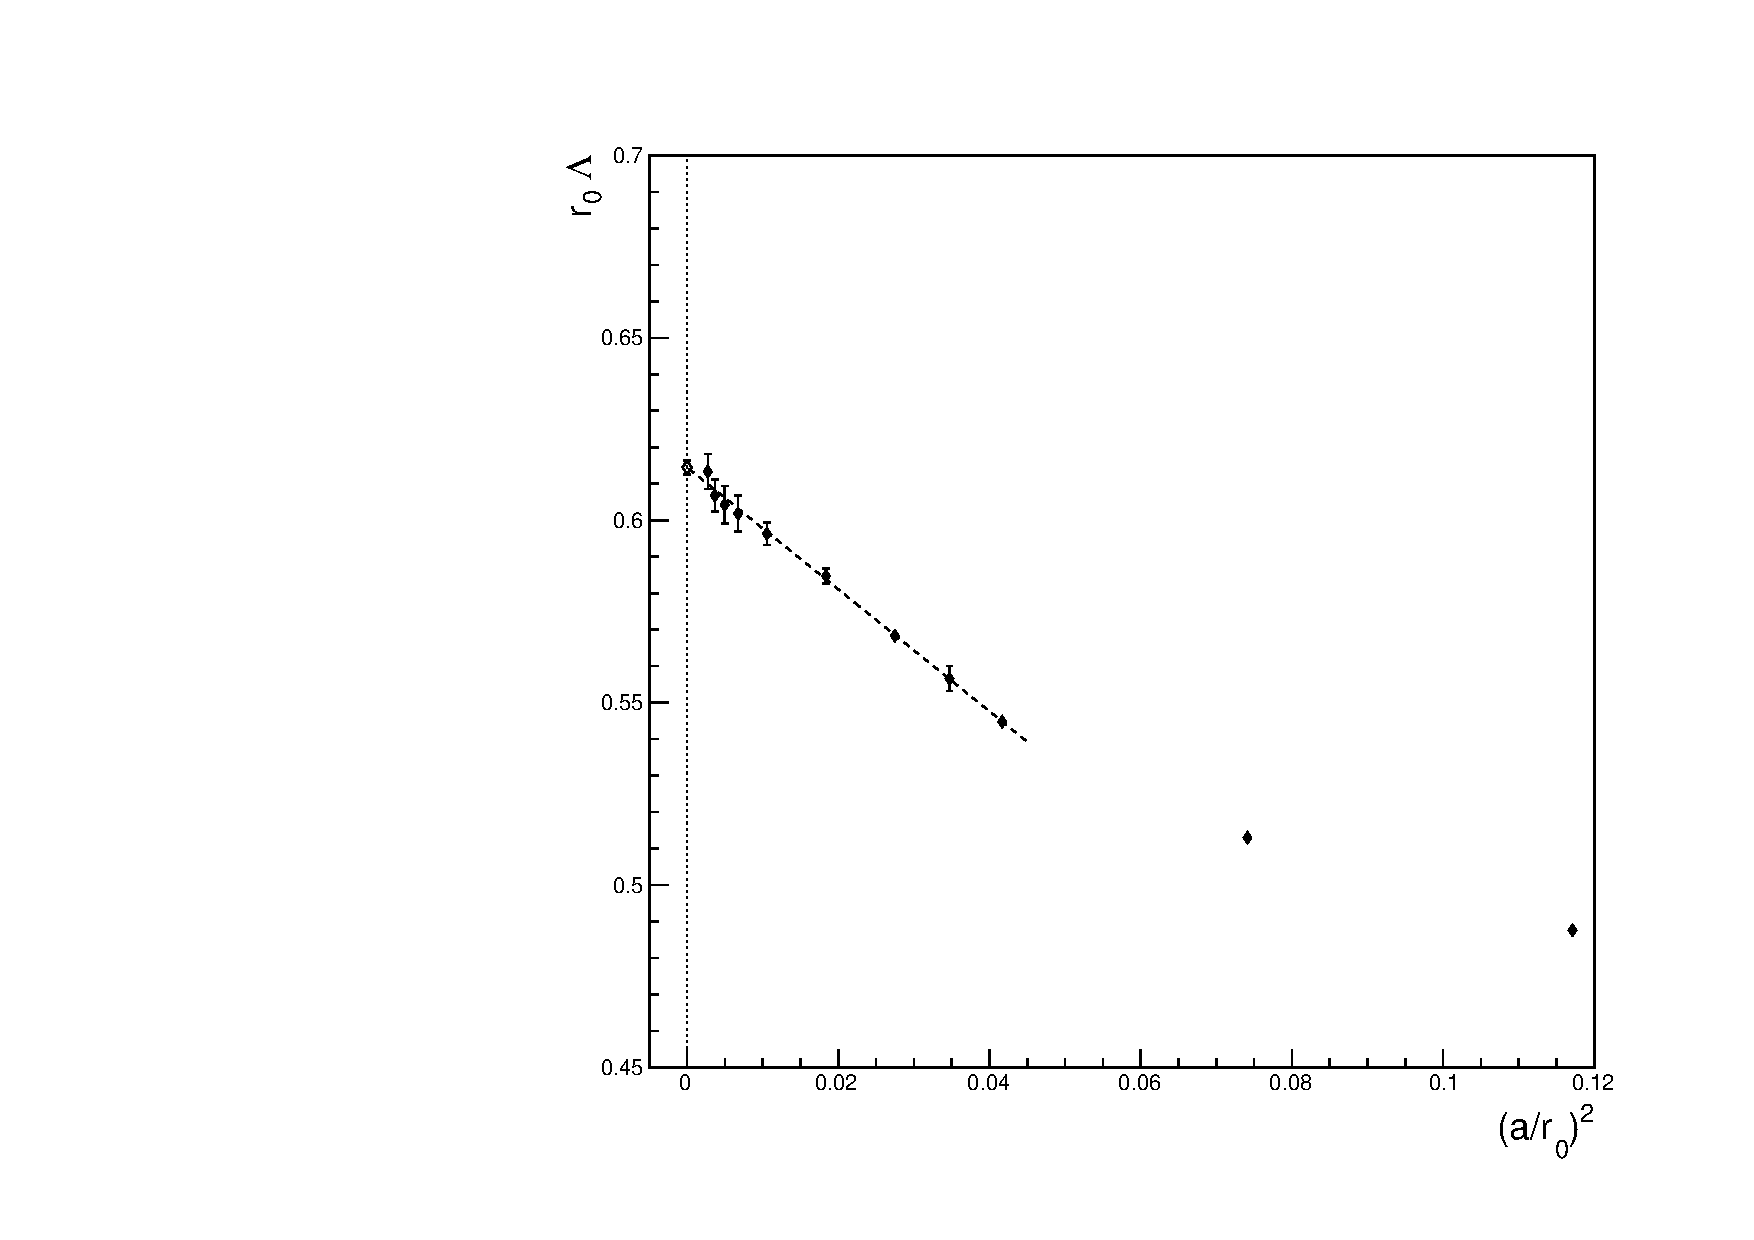
\includegraphics[width=0.50\textwidth]{methodIIPquenched.pdf}
  }
  \caption{Extrapolation of $r_0\Lambda_{(0)}^\msbar$ to the continuum limit with $n_f=0$ for Method II and Method IIP using 
the boosted coupling scheme.}
  \label{fig:method_II_IIP_quenched}
\end{center}
\end{figure}

Figure \ref{fig:methodI_boosted} shows that the boosted coupling scheme behaves linearly in the squared lattice spacing, at least for small 
values of $a$. Consequently, only the boosted coupling scheme will hereafter be considered. Higher order effects can be seen at larger values 
of $(a/r_0)^2$, so the continuum limit extrapolation is fit using only those datapoints with $(a/r_0)^2 < 0.06$.

The final result for $r_0 \Lambda_{(0)}^\msbar$ is calculated by taking the mean of the values for Methods I, II, and IIP. The 
statistical error is the standard deviation of the mean, and the systematic error is estimated from the spread of the 
three values, taken to be the sample standard deviation. The quoted value is thus\footnote{The ordering of the errors is (stat)(sys).}
\begin{equation} \label{eq:r0Lambda0_results} \begin{aligned}
r_0 \Lambda_{(0)}^\msbar = 0.6159(11)(31) .
\end{aligned} \end{equation}

which should be compared to the world average $r_0 \Lambda_{(0)}^\msbar = 0.62(2)$ \cite{Aoki:2013}. Using the value of $r_0$ given 
by eq. (\ref{eq:r0_value}), and combining the statistical and systematic errors of $r_0$ in quadrature 
(likewise with $r_0 \Lambda_{(2)}^\msbar$), the physical value for $\Lambda_{(2)}^\msbar$ is found to be
\begin{equation} \label{eq:Lambda0_results} \begin{aligned}
\Lambda_{(0)}^\msbar = 243(7)\ {\rm MeV} .
\end{aligned} \end{equation}

\section{$n_f=2$} \label{sec:nf2}

Table \ref{tab:r0a_P_data_extrap} contains the data used for extrapolating $r_0/a$ and $P$ to the chiral limit. The $r_0/a$ data (in the form
of $r_0 m_\pi$ and $am_\pi$) is taken from \cite{Bali:2012}, the $\kappa_c$ values are taken from \cite{Gockeler:2005}, and the plaquette 
values are taken from a QCDSF-UKQCD private database\footnote{D.\ Pleiter, private communication.}. The variables $\beta$ and $\kappa$ are 
put in by hand to the simulation, so the dataset contains multiple reoccurrences of the same values of $\beta$ and $\kappa$ where the sole
difference in input is the spatial and temporal extent of the lattice. Wherever these reoccurences appear, the lattice with the 
largest 4-volume is kept and the others are discarded. Table \ref{tab:r0a_P_data_extrap} also holds the $r_0/a$ and $P$ values in 
the chiral limit, extrapolated using the methods described in what follows.

For extrapolating $r_0/a$ to the chiral limit, a global fit is used \cite{Gockeler:2005}, paramaterized by 
\begin{equation} \label{eq:global_fit} \begin{aligned}
\ln \paren{\frac{r_0}{a}} = \bracket{a_{0,0}+a_{0,1}\beta}
 + \bracket{a_{1,0}+a_{1,1}\beta+a_{1,2}\beta^2}(am_q)
 + \bracket{a_{2,0}+a_{2,1}\beta+a_{2,2}\beta^2}(am_q)^2
\end{aligned} \end{equation}

where $am_q$ is calculated from $\kappa$ and $\kappa_c$ using eq. (\ref{eq:amq_relation}). Despite the lack of data for $r_0/a$ for
the smallest value of $\beta$, the global fit is what allows for the determination of $r_0/a$ at $\beta=5.20$. Figure 
\ref{fig:r0a_chiral_extrap} shows this global fit. 

The extrapolation of the average plaquette $P$ to the chiral limit is done using a simple quadratic fit in the bare quark mass 
for each value of $\beta$. Explicitly, the function
\begin{equation} \label{eq:nonglobal_fit} \begin{aligned}
\frac{r_0}{a}=b_0 + b_1(am_q) + b_2(am_q)^2 
\end{aligned} \end{equation}

\begin{table}[p!]
\begin{center}
\begin{tabular}{c c c c c c}
\hline 
\rule{0pt}{2ex}    
$\beta$ & $\kappa_c$ & $\kappa$ & Lattice & $r_0/a$ & $P$\\
\hline \hline
5.20 & 0.136008(15) & 0.13420 & $16^3 \times 32$ &     -          & 0.528994(58) \\
5.20 & 0.136008(15) & 0.13500 & $16^3 \times 32$ &     -          & 0.533670(40) \\
5.20 & 0.136008(15) & 0.13550 & $16^3 \times 32$ &     -          & 0.536250(30) \\
5.20 & 0.136008(15) & 0.13565 & $16^3 \times 32$ &     -          & \ 0.537070(100)\\
5.20 & 0.136008(15) & 0.13580 & $16^3 \times 32$ &     -          & 0.537670(30) \\  
\ 5.20$^\S$ & 0.13580\ \ \ \ \ \ \ \ & 0.13580 & - & 6.112(29) & \ 0.538625(117) \\ \rule{0pt}{3.0ex}

5.25\ \ & 0.136250(07) & 0.13460 & $16^3 \times 32$ & 6.602(56) & 0.538770(41) \\
5.25 & 0.136250(07) & 0.13520 & $16^3 \times 32$ & 6.603(62) & 0.541150(30) \\
5.25 & 0.136250(07) & 0.13575 & $24^3 \times 48$ & 6.600(56) & 0.543135(15) \\
5.25 & 0.136250(07) & 0.13600 & $24^3 \times 48$ & 6.603(65) & 0.544038(09) \\
5.25 & 0.136250(07) & 0.13620 & $32^3 \times 64$ & \ 6.600(116) & 0.544782(29) \\  
\ 5.25$^\S$ & 0.13620\ \ \ \ \ \ \ \ & 0.13580 & - & 6.593(32) & 0.544930(34) \\ \rule{0pt}{3.0ex}  

5.29\ \ & 0.136410(09) & 0.13400 & $16^3 \times 32$ & 7.004(57) & 0.542400(50) \\ 
5.29 & 0.136410(09) & 0.13500 & $16^3 \times 32$ & 7.004(59) & 0.545520(29) \\    
\ 5.29$^\dag$ & 0.136410(09) & 0.13550 & $12^3 \times 32$ & \ 7.004(104) & 0.547293(44) \\    
\ 5.29$^\dag$ & 0.136410(09) & 0.13550 & $16^3 \times 32$ & 7.005(67) & 0.547104(44) \\    
5.29 & 0.136410(09) & 0.13550 & $24^3 \times 48$ & 7.003(57) & 0.547094(23) \\    
\ 5.29$^\dag$ & 0.136410(09) & 0.13590 & $12^3 \times 32$ & \ 7.005(190) & 0.548569(59) \\    
\ 5.29$^\dag$ & 0.136410(09) & 0.13590 & $16^3 \times 32$ & 7.002(79) & 0.548317(30) \\    

5.29 & 0.136410(09) & 0.13590 & $24^3 \times 48$ & 7.002(56) & 0.548286(57) \\    
5.29 & 0.136410(09) & 0.13620 & $24^3 \times 48$ & 7.004(70) & 0.549187(16) \\    
\ 5.29$^\dag$ & 0.136410(09) & 0.13632 & $24^3 \times 48$ & 7.005(99) & 0.549542(09) \\    
\ 5.29$^\dag$ & 0.136410(09) & 0.13632 & $32^3 \times 64$ & 7.009(73) & 0.549541(08) \\    
5.29 & 0.136410(09) & 0.13632 & $40^3 \times 64$ & 7.000(61) & 0.549540(08) \\    
\ 5.29$^\dag$ & 0.136410(09) & 0.13640 & $40^3 \times 64$ & \ 7.015(136) & 0.549546(12) \\ 
5.29 & 0.136410(09) & 0.13640 & $48^3 \times 64$ & \ 7.000(136) & 0.549782(06) \\  
\ 5.29$^\S$ & 0.13580\ \ \ \ \ \ \ \ & 0.13580 & - & 7.005(34) & 0.549811(19) \\ \rule{0pt}{3.0ex} 
    
5.40\ \ & 0.136690(22) & 0.13500 & $24^3 \times 48$ & 8.285(75) & 0.559000(19) \\
5.40 & 0.136690(22) & 0.13560 & $24^3 \times 48$ & 8.287(79) & 0.560246(10) \\    
5.40 & 0.136690(22) & 0.13610 & $24^3 \times 48$ & 8.284(81) & 0.561281(08) \\    
5.40 & 0.136690(22) & 0.13625 & $24^3 \times 48$ & 8.286(83) & 0.561550(07) \\    
\ 5.40$^\dag$ & 0.136690(22) & 0.13640 & $24^3 \times 48$ & \ 8.283(106) & 0.561895(12) \\    
5.40 & 0.136690(22) & 0.13640 & $32^3 \times 64$ & 8.279(84) & 0.561887(10) \\    
\ 5.40$^\dag$ & 0.136690(22) & 0.13660 & $32^3 \times 64$ & \ 8.284(111) & 0.562278(05) \\    
5.40 & 0.136690(22) & 0.13660 & $48^3 \times 64$ & 8.281(93) & 0.562274(05) \\   
\ 5.40$^\S$ & 0.13580\ \ \ \ \ \ \ \ & 0.13580 & - & 8.275(40) & 0.56246(48) \\  
\hline
\end{tabular}
\end{center}
\caption{The $n_f=2$ dataset. Rows containing $\beta$-values 
marked with a `\dag' are not used in the fit, and rows containing $\beta$-values decorated with a `\S' are in the chiral limit.}
\label{tab:r0a_P_data_extrap}
\end{table}

\begin{figure}[p]
\begin{center}
  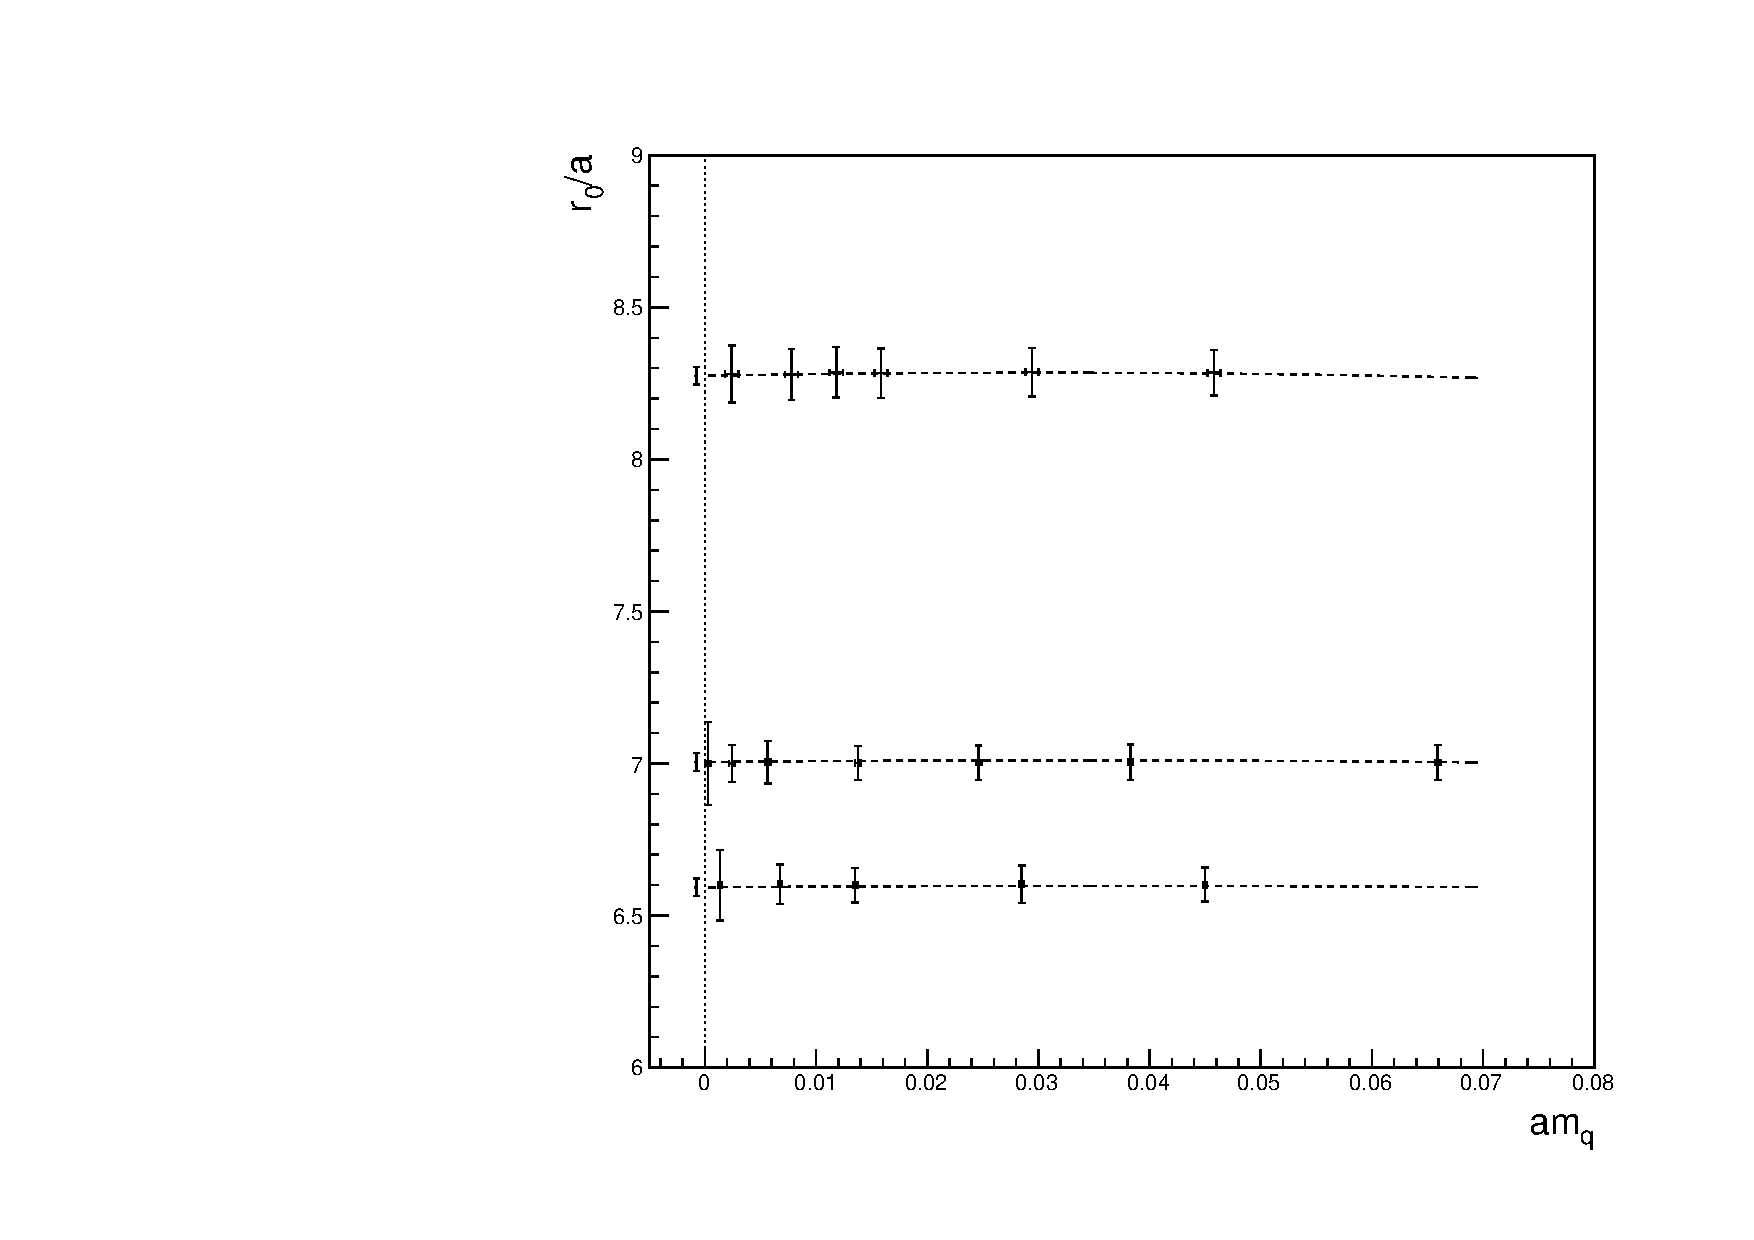
\includegraphics[width=4.0in]{r0_Over_a_Chiral_Extrap.pdf}
  \caption{Extrapolation of $r_0/a$ to the chiral limit using the global fit hypothesis. Extrapolated points are shifted left 
for aesthetic purposes.}
  \label{fig:r0a_chiral_extrap}
\end{center}
\end{figure}

\begin{figure}[p]
\begin{center}
  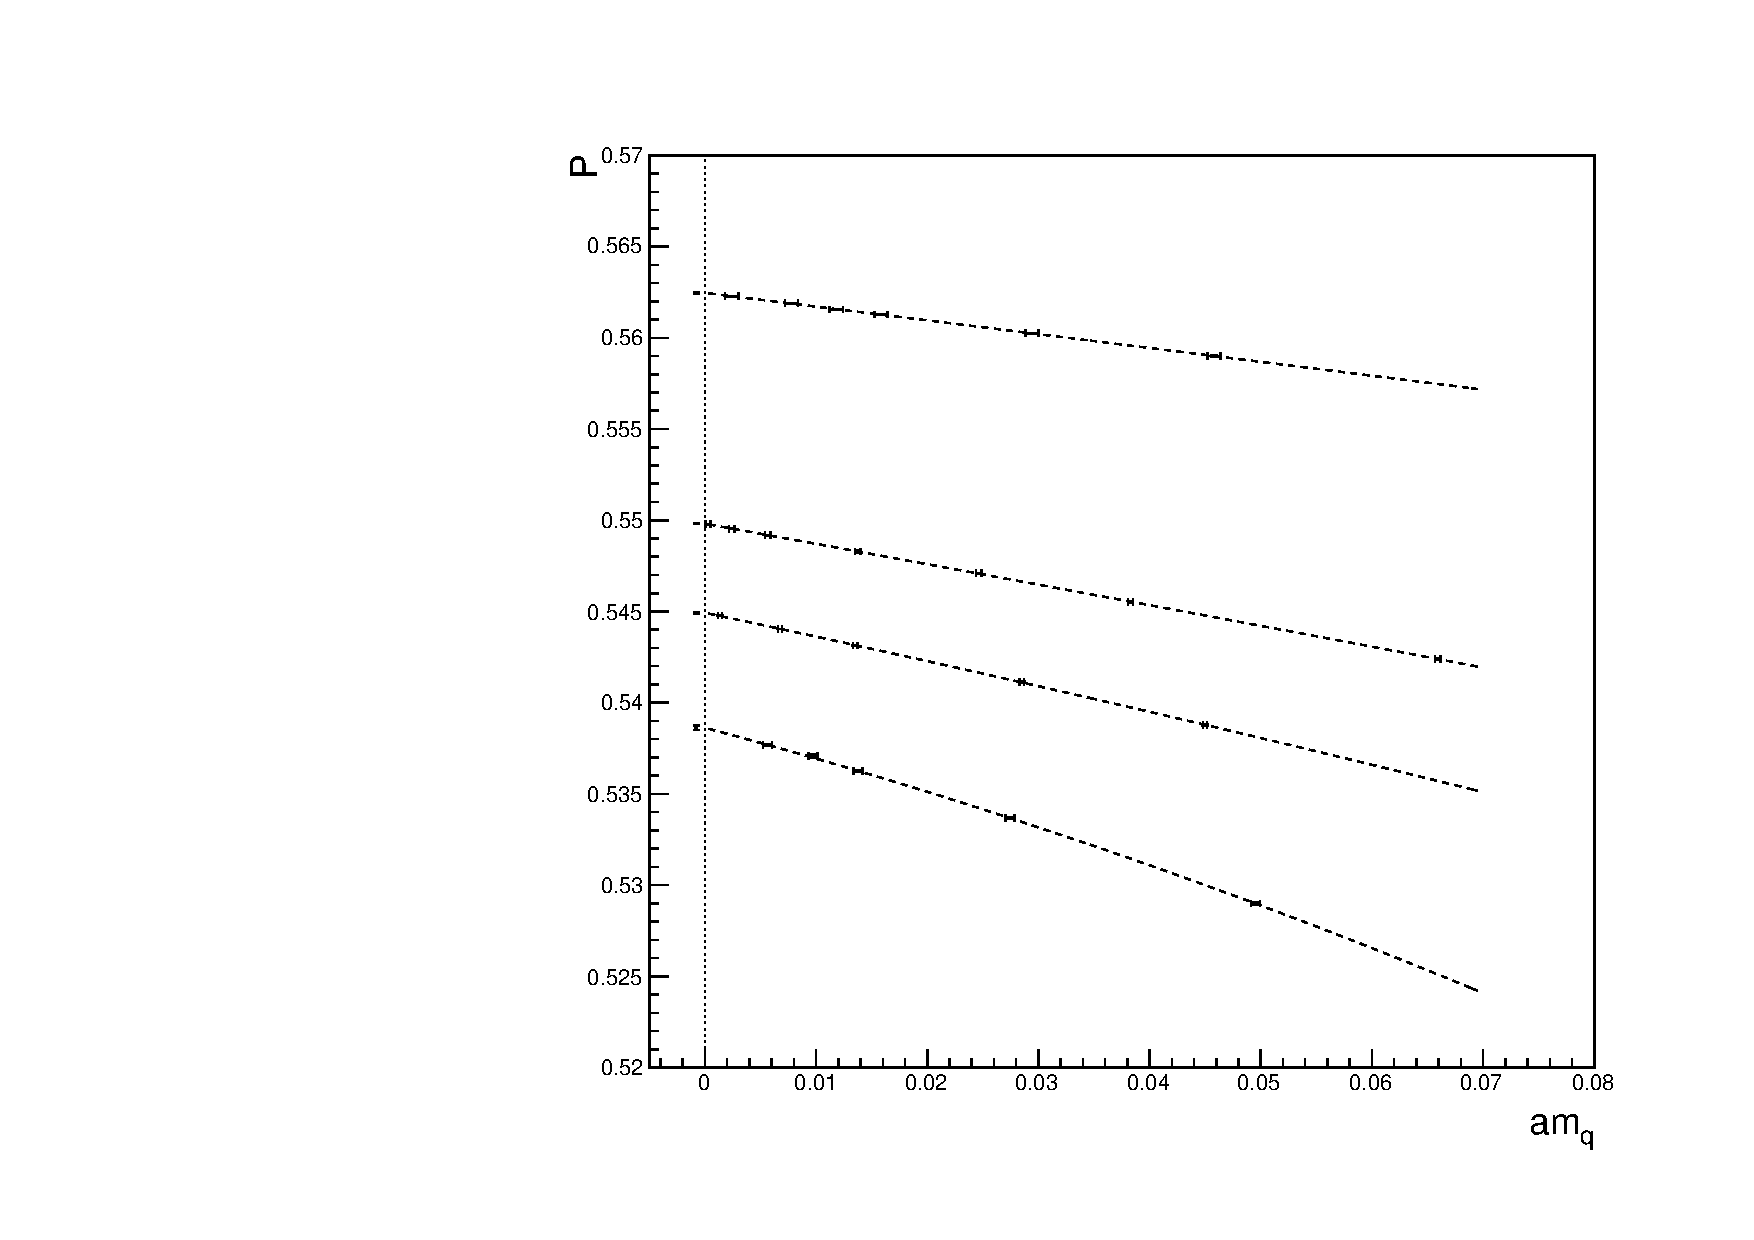
\includegraphics[width=4.0in]{Plaquette_Chiral_Extrap.pdf}
  \caption{Extrapolation of the average plaquette $P$ to the chiral limit. From the bottom, the fitted lines correspond to 
$\beta=$ 5.20, 5.25, 5.29, and 5.40. Extrapolated points are shifted left for aesthetic purposes.}
  \label{fig:plaquette_chiral_extrap}
\end{center}
\end{figure}

is fit for each value of $\beta$ in the set \{5.20,5.25,5.29,5.40\}. A plot of these fits are shown in Figure \ref{fig:plaquette_chiral_extrap}.

Using the chiral values for $r_0/a$ and $P$ marked with an `\S' in Figure \ref{tab:r0a_P_data_extrap}, $r_0\Lambda_{(2)}^\msbar$ can 
now be calculated for each value of the coupling $\beta$ and the continuum limit taken. These $r_0\Lambda_{(2)}^\msbar$ values are 
shown in Table \ref{tab:continuum_limit_nf2}, calculated using each of the methods introduced in \S\ref{sec:three_methods}.

\begin{figure}[h!]
\begin{center}
  \subfloat[\label{fig:method_I_II_III_nf2}]{
    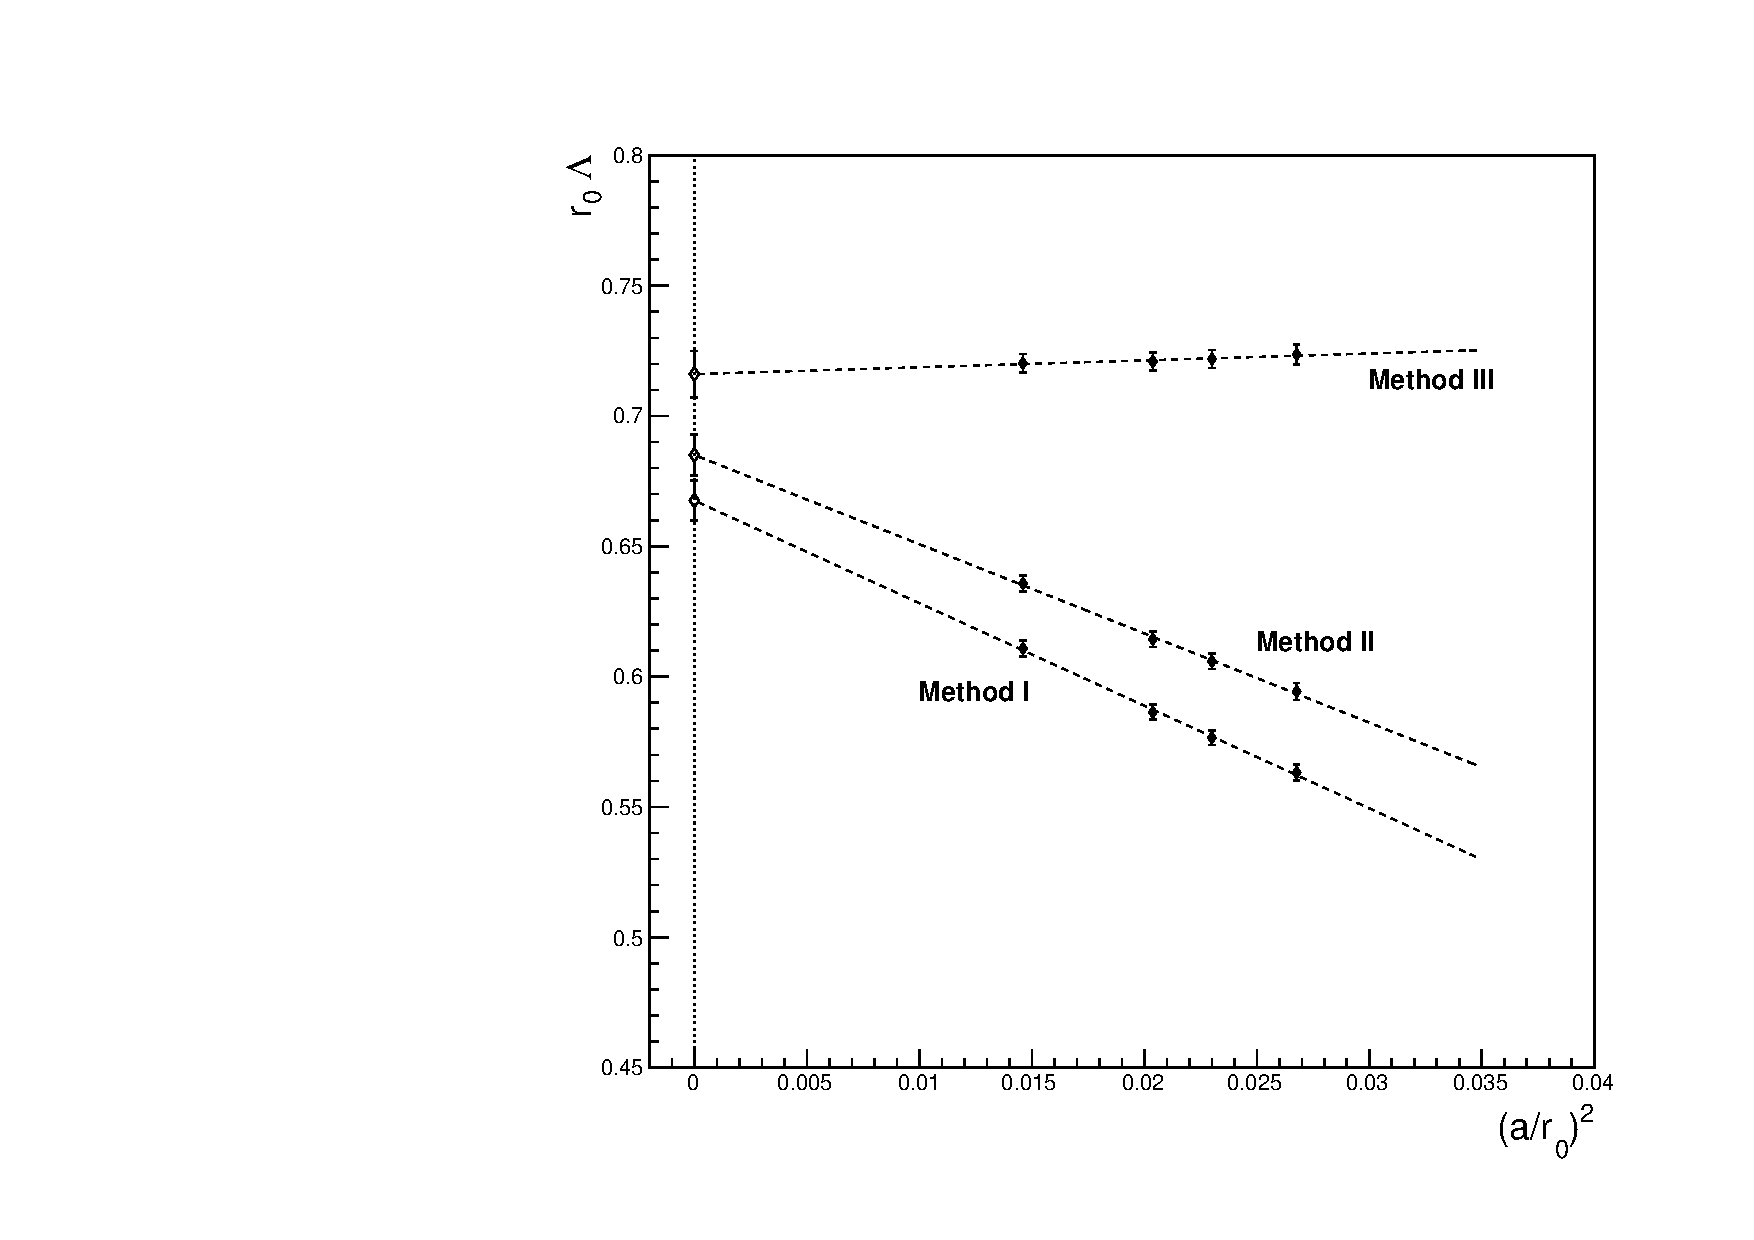
\includegraphics[width=0.50\textwidth]{method_I_II_III_nf=2.pdf}
  }
  \hspace{-0.27in}
  \subfloat[\label{fig:method_IIP_IIP_nf2}]{
    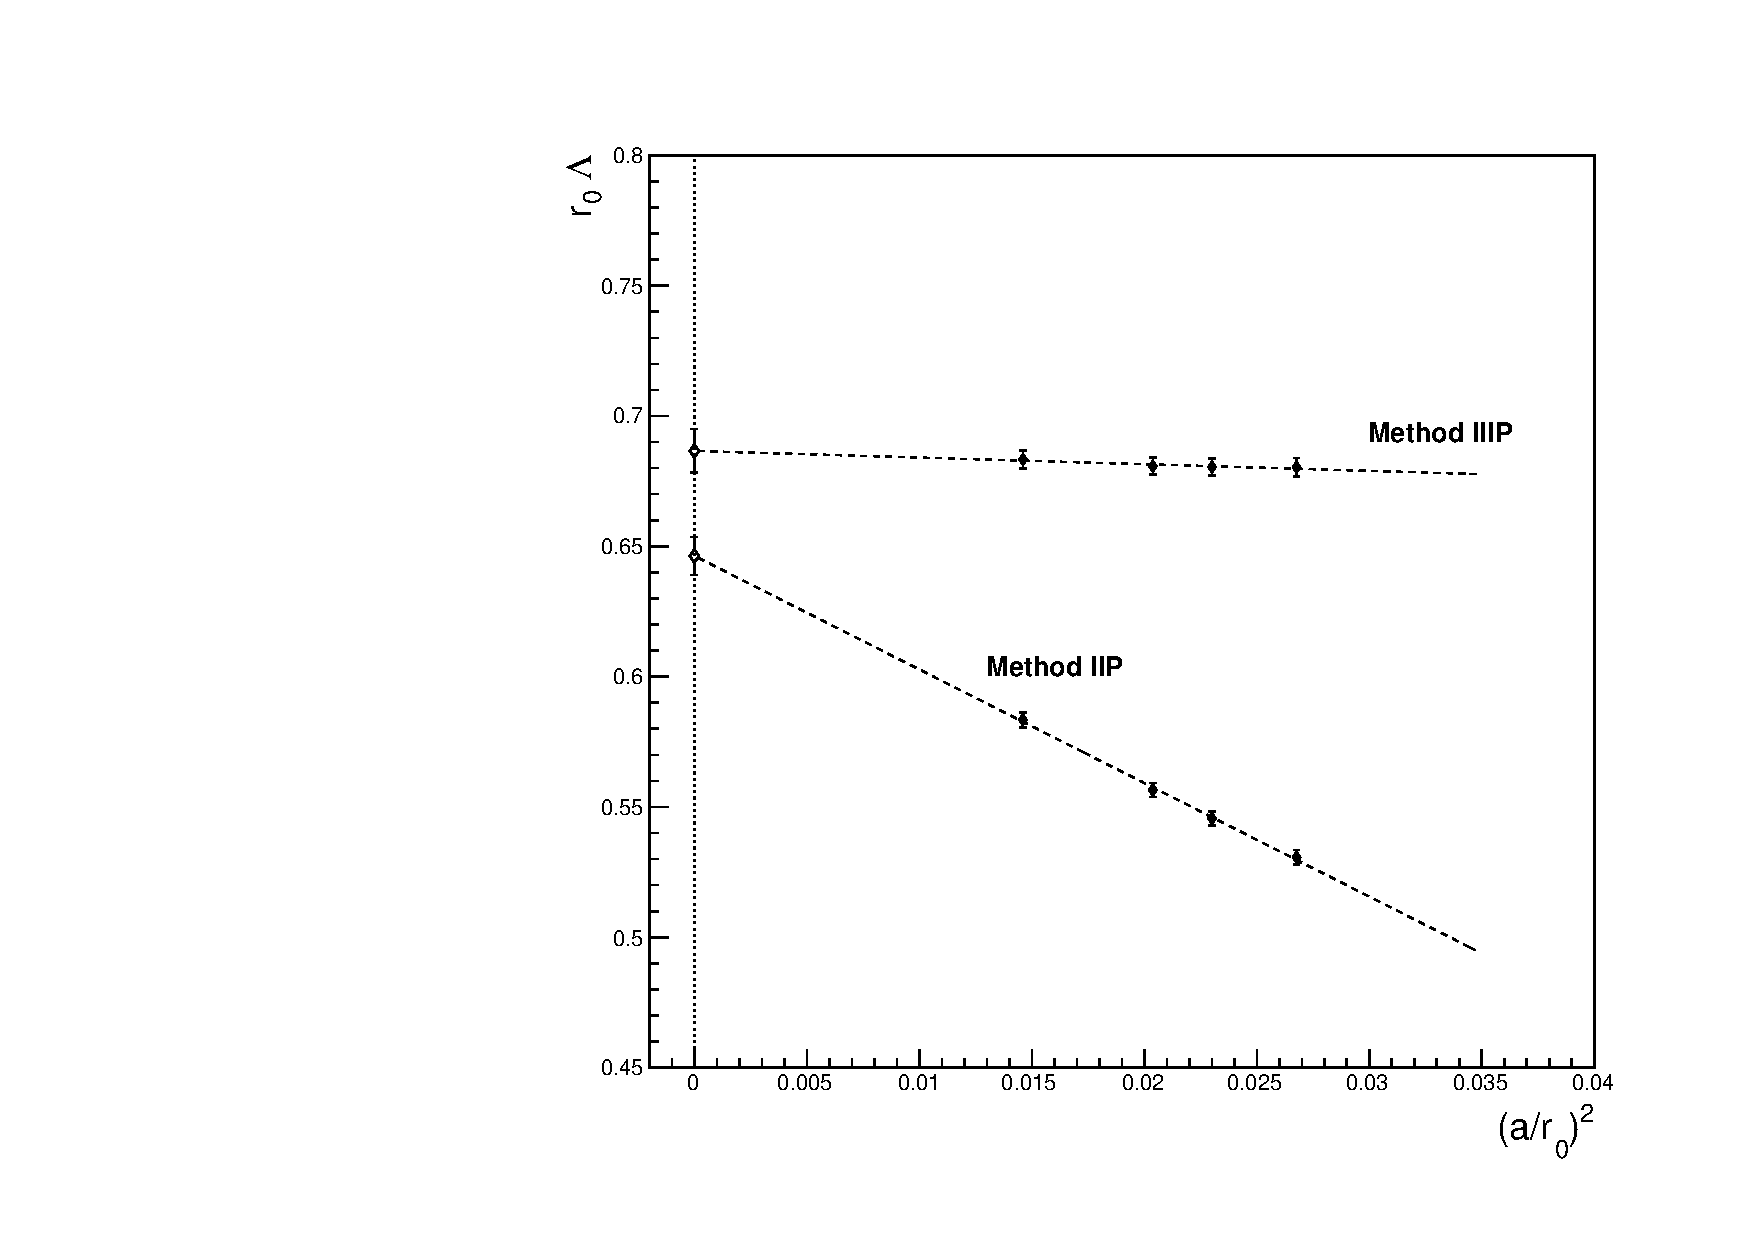
\includegraphics[width=0.50\textwidth]{method_IIP_IIIP_nf=2.pdf}
  }
  \caption{Extrapolation of $r_0\Lambda_{(2)}^\msbar$ to the continuum limit with $n_f=2$ for the three methods (left) as well
as the two Pad\'{e} improved methods (right).}
  \label{fig:method_II_IIP_nf2}
\end{center}
\end{figure}

\begin{table}[h!]
\begin{center}
\begin{tabular}{c c c c c c c c}
\hline 
\rule{0pt}{3ex}    
$\beta$ & $r_0\Lambda_{(2)}^\msbar$ I & $r_0\Lambda_{(2)}^\msbar$ II & $r_0\Lambda_{(2)}^\msbar$ IIP & $r_0\Lambda_{(2)}^\msbar$ III & $r_0\Lambda_{(2)}^\msbar$ IIIP \\
\hline \hline
5.20     & 0.5632(31) & 0.5943(32) & 0.5307(28) & 0.7236(39) & 0.6804(36) \\
5.25     & 0.5766(28) & 0.6059(29) & 0.5456(26) & 0.7219(35) & 0.6804(33) \\
5.29     & 0.5864(28) & 0.6144(30) & 0.5565(28) & 0.7209(35) & 0.6808(33) \\
5.40     & 0.6108(30) & 0.6357(32) & 0.5835(29) & 0.7203(36) & 0.6833(34) \\ \rule{0pt}{2.5ex}    
$\infty$ & 0.6675(77) & 0.6850(79) & 0.6463(73) & 0.7161(89) & 0.6866(84) \\
\hline
\end{tabular}
\end{center}
\caption{The $r_0\Lambda_{(2)}^\msbar$ values determined using the three methods plus the two Pad\'{e} improved methods. The last row shows 
extrapolated values in the continuum limit.}
\label{tab:continuum_limit_nf2}
\end{table}

As in \S\ref{sec:nf0}, the final result for $r_0 \Lambda_{(2)}^\msbar$ is calculated by taking the mean of the values from Methods 
I, II, IIP, III, and IIIP. The statistical error is given by the standard deviation of the mean, and the systematic error given by
 the sample standard deviation. The quoted value for $r_0 \Lambda_{(2)}^\msbar$,
to be compared to the world average $r_0 \Lambda_{(2)}^\msbar = 0.79(_{-13}^{+\ 5})$ \cite{Aoki:2013},  is thus
\begin{equation} \label{eq:r0Lambda2_results} \begin{aligned}
r_0 \Lambda_{(2)}^\msbar = 0.6803(36)(258) .
\end{aligned} \end{equation}

The errors affixed to this result show that the statistics for $n_f=2$ vacuum configurations have reached a level of precision that 
allow the various methods to be distinguished, whereas this was not the case in \cite{Gockeler:2005}. The systematic error drowns 
out the statistical error, suggesting that further improvements in simulation technology would be meaningless without first 
improving the methods used to calculate $r_0 \Lambda_{(2)}^\msbar$.

Combining the statistical and systematic errors of $r_0$ in quadrature, and likewise in $r_0 \Lambda_{(2)}^\msbar$, the physical value 
for $\Lambda_{(2)}^\msbar$ is
\begin{equation} \label{eq:Lambda2_results} \begin{aligned}
\Lambda_{(2)}^\msbar = 268(13)\ {\rm MeV} .
\end{aligned} \end{equation}

\section{Evolving $\alpha_\msbar$ to $m_Z$} \label{sec:evolving_alpha}

Equipped now with physical values for $\Lambda_{(0)}^\msbar$ and $\Lambda_{(2)}^\msbar$, the methods of \S\ref{sec:crossing_thresholds} 
can be used to find the final result for $\alpha_\msbar^{(n_f=5)}$. Beginning by crossing the strange threshold as described in 
\S\ref{sec:strange_threshold}, the value for the ratio $\Lambda_{(2)}^\msbar/ \Lambda_{(0)}^\msbar$ is\footnote{This ratio is 
calculated directly from the $r_0 \Lambda_{(n_f)}^\msbar$ values since it is more precise.}
\begin{equation} \label{eq:rat20_results} \begin{aligned}
\frac{\Lambda_{(2)}^\msbar}{\Lambda_{(0)}^\msbar} = 1.104(43).
\end{aligned} \end{equation}

Inputting this value into the matching curves shown in Figure \ref{fig:rat32_v_rat20_good}, the ratio 
\begin{equation} \label{eq:rat32_results} \begin{aligned}
\frac{\Lambda_{(3)}^\msbar}{\Lambda_{(2)}^\msbar} = 1.068(28)(07)
\end{aligned} \end{equation}

is found. The quoted central value is the mean of the values given by considering each of the 1-, 2-, and 3-loop curves in turn. The 
first error comes from numerically propagating the error from eq. (\ref{eq:rat20_results}) through each of the curves then 
taking the standard deviation of the mean, while the second error comes from the sample standard deviation of the 1-, 2-, and 3-loop 
$\Lambda_{(3)}^\msbar / \Lambda_{(2)}^\msbar $ values.

Using the ratio $\Lambda_{(3)}^\msbar / \Lambda_{(2)}^\msbar$ given in eq. (\ref{eq:rat32_results}) and the value for 
$r_0 \Lambda_{(2)}^\msbar$ given in eq. (\ref{eq:r0Lambda2_results}), it is found that 
\begin{equation} \label{eq:r0Lambda3_results} \begin{aligned}
\Lambda_{(3)}^\msbar = 0.727(32),
\end{aligned} \end{equation}

which should be compared to the world average $r_0 \Lambda_{(3)}^\msbar = 0.81(4)$ \cite{Aoki:2013}. In physical units,
\begin{equation} \label{eq:Lambda3_results} \begin{aligned}
\Lambda_{(3)}^\msbar = 286(16)\ {\rm MeV} ,
\end{aligned} \end{equation}

whereas the world average is $\Lambda_{(3)}^\msbar = 339(17)$ \cite{Aoki:2013}. Again, the statistical and systematic errors of 
any variable were added in quadrature before propagating through the error.

The remaining thresholds will be crossed using the method of \S\ref{sec:charm_beauty_thresholds}. The quoted errors take into
account the error from $\Lambda_{(3)}^\msbar$ as well as the errors on the quark masses (see eq. (\ref{eq:z_quark_masses})).
First, the charm threshold is crossed, giving
\begin{equation} \label{eq:Lambda4_results} \begin{aligned}
\Lambda_{(4)}^\msbar =  244(16) \ {\rm MeV} .
\end{aligned} \end{equation}

Then the beauty threshold is crossed, resulting in
\begin{equation} \label{eq:Lambda5_results} \begin{aligned}
\Lambda_{(5)}^\msbar =  172(13) \ {\rm MeV} .
\end{aligned} \end{equation}

Finally, the strong coupling constant $\alpha_\msbar^{(n_f=5)}$ is evaluated at the mass of the Z boson, giving the final result
\begin{equation} \label{eq:alpha_msbar_result} \begin{aligned}
\alpha_\msbar^{(n_f=5)}(m_Z) =  0.1146(13) .
\end{aligned} \end{equation}

\begin{figure}[h!]
\begin{center}
  \subfloat[\label{fig:compare_alphas}]{
    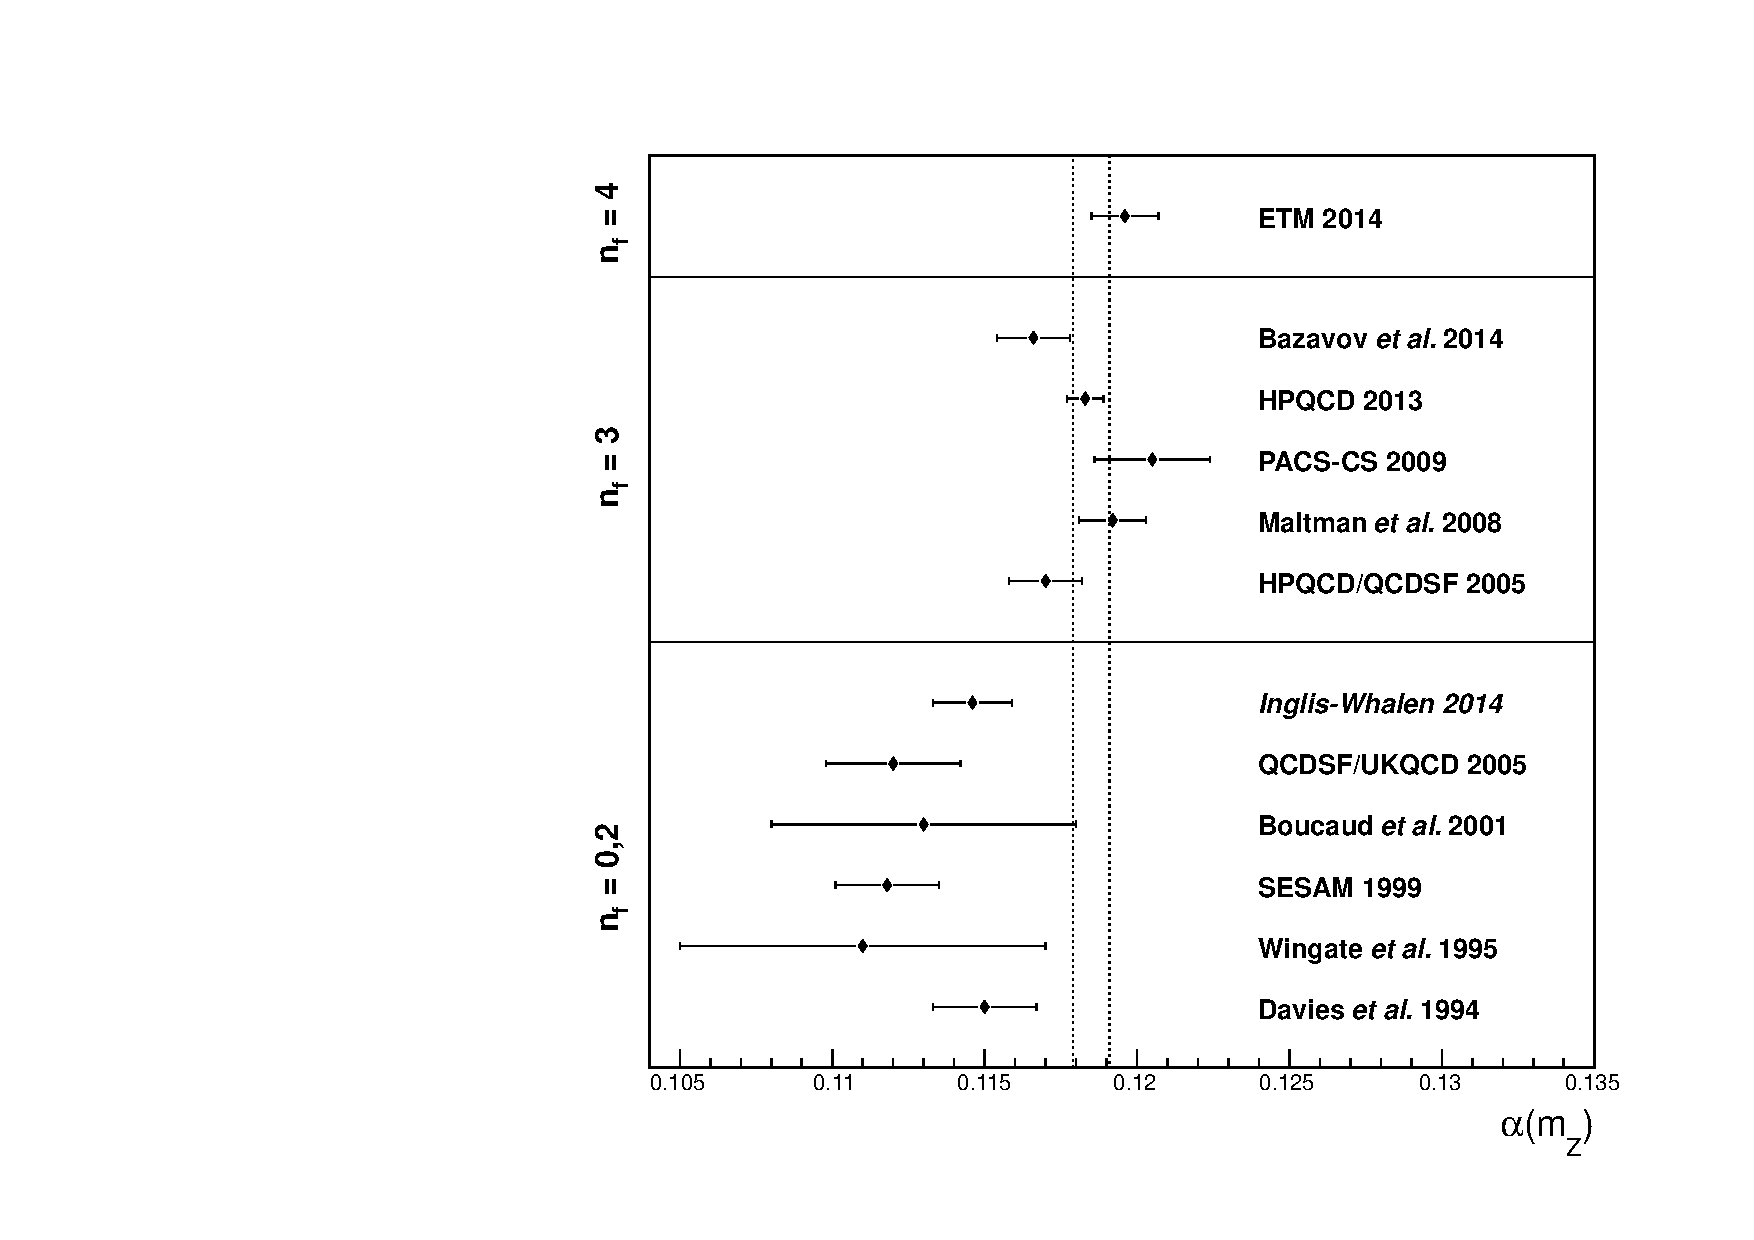
\includegraphics[width=0.50\textwidth]{compare_alphas.pdf}
  }
  \hspace{-0.27in}
  \subfloat[\label{fig:compare_lambdas}]{
    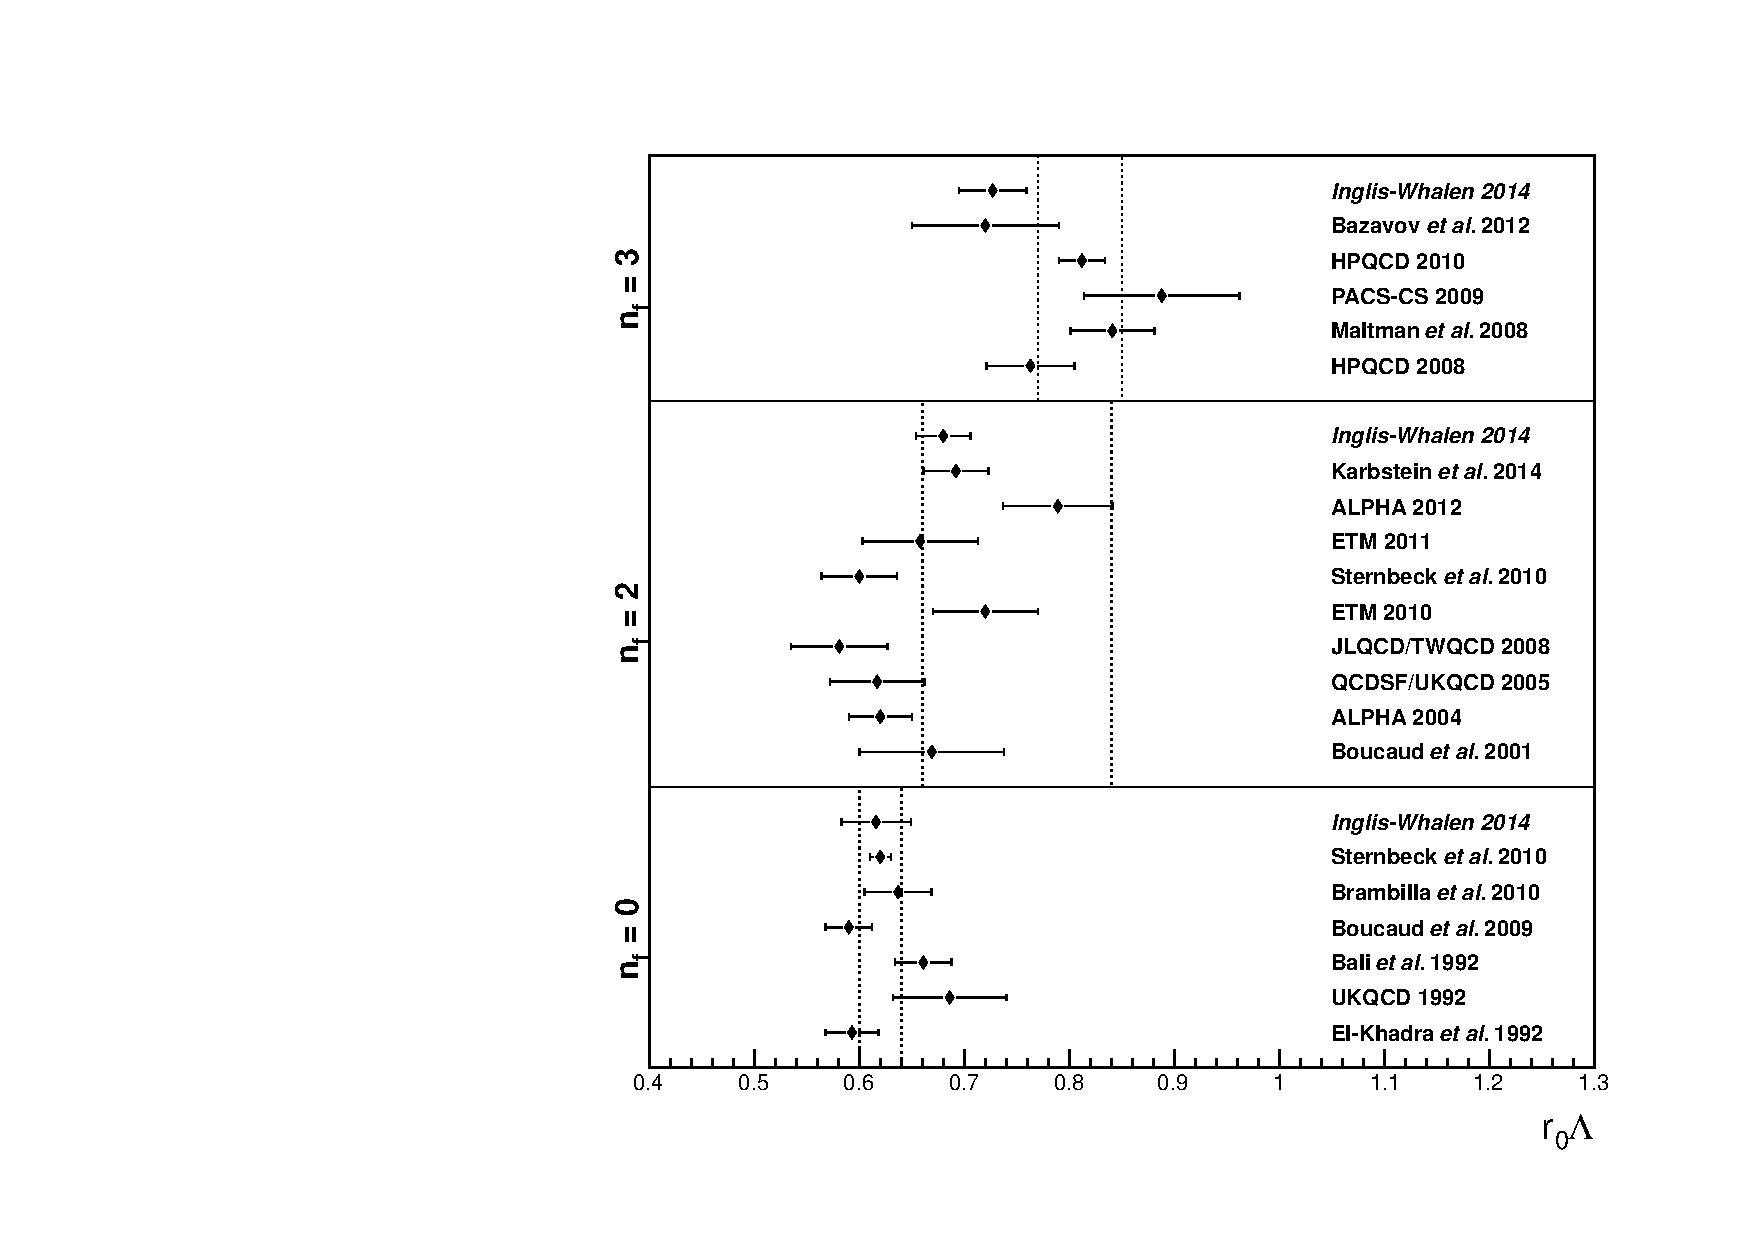
\includegraphics[width=0.50\textwidth]{compare_lambdas.pdf}
  }
  \caption{This work's values of $\alpha_\msbar^{(n_f=5)}(m_Z)$ (left) and $r_0\Lambda_{(n_f)}^\msbar$ (right) compared 
to other lattice determinations in the literature. The vertical dashed lines represent the 1-$\sigma$ confidence interval for the 
PDG's (left) and the FLAG Working Group's (right) current world average. Bazavov {\it et al.} 2014 is taken from \cite{Bazavov:2014},
Karbstein 2014 is taken from \cite{Karbstein:2014}, and the remaining values are taken from the FLAG review \cite{Aoki:2013}. }
  \label{fig:compare_values}
\end{center}
\end{figure}

%%% --------------------------------------------------------------------

% This was included by mistake in the final manuscript

\blfootnote{ Left -- Bazavov {\it et al.} 2014 is taken from \cite{Bazavov:2014}, with the other values taken from the FLAG review \cite{Aoki:2013}.
%\cite{Blossier:2013,Bazavov:2014,McNeile:2010,Aoki:2009,Maltman:2008,Mason:2005,Gockeler:2005,Boucaud:2001,
%Spitz:1999,Wingate:1995,Davies:1994} (top to bottom). 
\\ Right -- Karbstein 2014 is taken from \cite{Karbstein:2014}, with the remaining
values taken from the FLAG review \cite{Aoki:2013}, which heavily interpreted the original papers. See references therein for more details. 
%which interpreted the values from the original papers \cite{Bazavov:2012,McNeile:2012,
%Aoki:2009,Maltman:2008,Mason:2005,Fritzsch:2012,Constantinou:2010} (top to bottom).
}

%%% --------------------------------------------------------------------

\chapter{Discussion} \label{sec:discussion}

This paper closely follows the methods of \cite{Gockeler:2005}, and as such it was important to replicate the results therein before
progressing to the analysis of the newly available data. This goal was achieved, but in the process a few minor differences were found. 
First, and of negligible numerical difference, was the fact that the four-loop QCD 
beta function was integrated numerically in \cite{Gockeler:2005}, whereas in this work the exact form of eq. (\ref{eq:beta_integ_NLloop})
was used. Second, the conversion from the boosted coupling scheme to the $\overline{MS}$ scheme in \cite{Gockeler:2005} was done using
the reciprocal expansion of eq. (\ref{eq:inverse_alpha_conversion}), but in this work the conversion was done using the direct expansion of eq. 
(\ref{eq:alpha_conversion}). This caused minor differences from the values of $r_0 \Lambda_{(0)}^\msbar$ shown in Table
\ref{tab:quenched_data}, but the continuum limit values agreed within error bars. Third, \cite{Gockeler:2005} directly integrated the 
Pad\'{e} improved beta function in eq. (\ref{eq:beta_31_pade}), and found a closed form expression for the integral. In contrast, this work 
continued to use eq. (\ref{eq:beta_integ_NLloop}) as the closed form expression for the integral, using the estimated beta function 
coefficient $\beta_3^S \approx (\beta_3^S)^2/\beta_1$. Again, this difference caused the calculated $r_0 \Lambda_{(2)}^\msbar$ values 
to slightly differ, but the continuum limit values agreed within error bars. Fourth, and perhaps the most interesting difference, is that 
the matching curves of Figure $\ref{fig:rat32_v_rat20_bad}$ were entirely smooth in \cite{Gockeler:2005}. It can be shown analytically
that the 1-loop value for $\Lambda_{(2)}/\Lambda_{(0)} \rightarrow 1.05144$ as $\alpha_\qqbar \rightarrow \infty$, so the author will
remain agnostic as to the methods used by the authors of \cite{Gockeler:2005} to generate their matching curves. Finally, the authors
of \cite{Gockeler:2005} used a simple $\chi^2$ fitting algorithm to determine fitted values and their associated errors. However, the 
datasets do not contain error free x-values (i.e $(a/r_0)^2$, $am_q$). To properly take these errors into account,
the modified variance approach was used\footnote{Recommended by CERN's ROOT package, see \\
http://root.cern.ch/root/html/TGraph.html\#TGraph:Chisquare .}, which replaces the $\sigma_{y_i}^2$ in the denominator of the $\chi^2$ 
definition with $\sigma_{y_i}^2+(\sigma_{x_i} f'(x_i))^2$, where $f'(x_i)$ is the first derivative of the fitted function evaluated at 
the point $x_i$. This had only a neglible effect on the extrapolated values, but increased their associated errors.

The main motivation for this paper was the new value of $r_0$, as well as the new values for $r_0/a$. The only equation where
the new $r_0$ value had any effect on the final result for $\alpha_\msbar^{(n_f=5)}(m_Z)$ was eq. (\ref{eq:Lambda3_results}). If the
previous value $r_0=0.473(33) {\rm fm}$ \cite{Gockeler:2005} were to be used, $\Lambda_{(3)}^\msbar$ would increase by 6\% of the 
value found in this work. $\Lambda_{(3)}^\msbar$ would still not agree with the world average, though it would be pushed to a high enough
value for error bars to overlap. This increase $\Lambda_{(3)}^\msbar$ would in turn increase the final $\alpha_\msbar^{(n_f=5)}(m_Z)$ value,
but still not enough to agree with the world average.

The effects stemming from the new $r_0/a$ values are much more significant. First, the resulting $r_0 \Lambda_{(2)}^\msbar$ value is much
higher than in \cite{Gockeler:2005}, where it was found that $r_0 \Lambda_{(2)}^\msbar = 0.617(45)$. This low value was propagated through 
the matching procedure, giving $r_0 \Lambda_{(2)}^\msbar = 0.616(35)$, and finally $\alpha_\msbar^{(n_f=5)}=0.1120(22)$. The new $r_0/a$ 
values were crucial to boosting up the $r_0 \Lambda_{(2)}^\msbar$ in the chiral limit so that they could reach a value of 
$r_0 \Lambda_{(2)}^\msbar$ in the continuum limit that agreed with the FLAG world average.

Secondly, and unexpectedly, the new $r_0/a$ data produced a significantly cleaner global fit extrapolation to the chiral limit for
the $r_0/a$ values themselves (see Figure \ref{fig:r0a_chiral_extrap}). In \cite{Gockeler:2005}, each of the $a_{i,j}$ fit parameters 
of eq. (\ref{eq:global_fit}) were needed to properly fit the data. In this work, however, the $r_0/a$ values were almost perfectly 
independent of the bare quark mass. As a result, if the parameters $a_{1,j}$ and $a_{2,j}$ are fixed to zero, the extrapolated 
$r_0/a$ values in the chiral limit change by less 0.1\%. This difference is completely obscured by the statistical noise. 

Returning to the three methods of \S\ref{sec:three_methods}, it is interesting to see the effect that the choice of scale has 
on the continuum limit value for $r_0 \Lambda_{(0)}^\msbar$ (see Figures \ref{fig:method_I_stability} and \ref{fig:method_II_stability}).
It would appear that any value of $r_0 \Lambda_{(0)}^\msbar$ could be found given the right scale. Yet the chosen scales are somehow
unique, knowing now that they correctly reproduce the world average value of $r_0 \Lambda_{(0)}^\msbar$. As explained
in \S\ref{sec:method_I}, the region where the slope is smallest is a good choice for $\mu$, but there is no reason to believe that
it is the \emph{best} value for $\mu$. In hindsight, it would have also been interesting to plot similar stability curves for 
$r_0 \Lambda_{(2)}^\msbar$ in the continuum limit.

Still, it is reassuring to see that the values of $r_0 \Lambda_{(0)}^\msbar$ and $r_0 \Lambda_{(2)}^\msbar$ shown 
in eqs. (\ref{eq:r0Lambda0_results}) and (\ref{eq:r0Lambda2_results}) the world average values. This indicates that the methods used to 
analyze the $n_f=0$ and $n_f=2$ datasets work as designed. Unfortunately, this good agreement is not reflected in the value found for 
$r_0 \Lambda_{(3)}^\msbar$. Apparently the matching procedure of \S\ref{sec:strange_threshold} did not perform as well as could be hoped.

Yet this appears to be a common theme amongst $n_f=0$ and $n_f=2$ lattice calculations. Figure \ref{fig:compare_alphas} shows that 
when $n_f=0$ and $n_f=2$ simulations are used to calculate $\alpha_\msbar^{(n_f=5)}(m_Z)$, the resulting values lie systematically
below the PDG's current world average. While it is tempting to conclude that the transition into the $n_f=3$ regime is the uniting stumbling 
block for these low-$n_f$ lattice studies, it has also been nearly 10 years since $n_f=2+1$ simulations became available. This has
made it unnecessary to cross the strange threshold at all, causing $n_f=0$ and $n_f=2$ simulations to fall out of fashion as a tool
for calculating $\alpha_\msbar^{(n_f=5)}(m_Z)$. One could argue that the advance of computational and theoretical techniques alone 
is the cause of the gap between the values of $\alpha_\msbar^{(n_f=5)}(m_Z)$ determined using $n_f=0$ and $n_f=2$ simulations and those 
values found using $n_f=2+1$ or $n_f=2+1+1$ simulations.

Perhaps a more decisive conclusion can be made. Papers continue to be written for the purpose of determining 
$r_0 \Lambda_{(0)}^\msbar$ and $r_0 \Lambda_{(2)}^\msbar$, as shown in Figure \ref{fig:compare_lambdas}.
Since 2005, the values of $r_0 \Lambda_{(0)}^\msbar$ have remained mostly constant, but $r_0 \Lambda_{(2)}^\msbar$ values have been 
skewed to a higher value by the few most recent data points. This can only be attributed to improved computational and theoretical 
methods. To see if crossing the strange threshold remains a barrier for calculating $r_0 \Lambda_{(3)}^\msbar$ using 
state-of-the-art $r_0 \Lambda_{(0)}^\msbar$ and $r_0 \Lambda_{(2)}^\msbar$ values, a crude estimation procedure is employed. 

If one takes the central values of the FLAG confidence intervals for $r_0 \Lambda_{(0)}^\msbar$ (0.62) and $r_0 \Lambda_{(2)}^\msbar$ (0.75) 
then use their ratio as input to the matching curves of Figure \ref{fig:rat32_v_rat20_good}, one finds $r_0 \Lambda_{(3)}^\msbar = 0.85$. 
This lies at the upper edge of the confidence interval for $r_0 \Lambda_{(3)}^\msbar$. Converting to a physical value for 
$\Lambda_{(3)}^\msbar$ with the new $r_0$ value of eq. (\ref{eq:r0_value}) and running the coupling constant up to the Z mass,
it is found that $\alpha_\msbar^{(n_f)}(m_Z)=0.1181$. This agrees well with PDG's world average. 

While this rough estimation is not meant to be conclusive, it convincingly shows that the existing matching procedure used to cross the strange 
threshold performs as expected for modern $n_f=0$ and $n_f=2$ simulations. However, it remains plausible that the $r_0 \Lambda_{(0)}^\msbar$ 
and $r_0 \Lambda_{(2)}^\msbar$ determined in this paper would produce a better result for $\alpha_\msbar^{(n_f=5)}(m_Z)$ if a different
matching procedure were used to cross the strange threshold. 

\chapter{Conclusions} \label{sec:conclusions}

This work aimed to determine the strong coupling constant $\alpha_\msbar^{(n_f=5)}(m_Z)$. 

The datasets used in this paper were drawn from the literature. Both $n_f=0$ and $n_f=2$ datasets were used. The $n_f=2$ datasets employed
Wilson fermions, non-perturbatively improved with the Sheikholeslami-Wohlert action. To set the scale, a newly
determined value of $r_0$ was used, though this pushed results further away from world averages. Updated values of the dimensionless 
inverse lattice spacing $r_0/a$ were also used, which played a key role in achieving a higher value for $r_0 \Lambda_{(2)}^\msbar$ 
in comparison to that found in \cite{Gockeler:2005}.

Due to the high statistics of the datasets, the three methods (plus the two Pad'{e} improved methods) could be distinguished from one another.
This made the systematic uncertainty larger than the statistical uncertainty for both $r_0 \Lambda_{(0)}^\msbar$ and 
$r_0 \Lambda_{(2)}^\msbar$ in the continuum limit, implying that improving lattice statistics would be fruitless unless accompanied by
a similar inprovement in the methodology.

The three methods (plus the two Pad\'{e} improved methods) resulted in finding the values $r_0 \Lambda_{(0)}^\msbar = 0.6159(11)(31)$ and
$r_0 \Lambda_{(2)}^\msbar = 0.6803(36)(258)$. Both of these values agreed with the FLAG world averages.

The matching procedure across the strange threshold involved assuming an $n_f$-independent static quark force. Due to the break down
of perturbation theory at the measured value of $\Lambda_{(2)}^\msbar/\Lambda_{(0)}^\msbar$, the procedure required an extrapolation
past the point where $\alpha_\qqbar \rightarrow \infty$. This gave the result $r_0 \Lambda_{(3)}^\msbar = 0.727(32)$. This did not agree
with the FLAG world average, but it was argued that this might not represent a failure in the matching procedure.

The strong coupling constant was run up to the scale of the Z mass, and was found to be $\alpha_\msbar^{(n_f=5)}(m_Z)=0.1146(13)$. This
did not agree with the PDG world average.

\appendix
% the appendix command just changes heading styles for appendices.

\chapter{Stability Analysis Details} \label{sec:stab_anal}

This section briefly outlines the equations used to find $r_0 \Lambda_{(0)}^\msbar$ as a function of the ratio of scales, as shown in Figures
\ref{fig:method_I_stability} and \ref{fig:method_II_stability}. Considering first Method I, let $R \equiv \mu / \mu_\one$. This implies, 
from eq. (\ref{eq:scale_choice_I}), that
\begin{equation} \label{eq:stab_anal1_I} \begin{aligned}
\mu = \frac{R}{a} \exp \paren{\frac{t_1^\boost}{2\beta_0}} .
\end{aligned} \end{equation}

Inserting this into eq. (\ref{eq:d_t_relations}), 
\begin{equation} \label{eq:stab_anal2_I} \begin{aligned}
d_1^\boost&=-2\beta_0\ln R \\
d_2^\boost&=t_2^\boost-\frac{\beta_1}{\beta_0}t_1^\boost-2\beta_1 \ln R + 4 \beta_0^2 \ln^2 R .
\end{aligned} \end{equation}

Using these $d_i$ coefficients, $\alpha_\boost$ is converted to $\alpha_\msbar$, and inserted into the central equation
\begin{equation} \label{eq:stab_anal3_I} \begin{aligned}
r_0 \Lambda_{(0)}^\msbar (R) = R \paren{ \frac{r_0}{a} } \exp{\paren{\frac{t_1^\boost}{2\beta_0}}} \frac{1}{M_{(0)}^\msbar (\alpha_\msbar(R)) } .
\end{aligned} \end{equation}

To plot $r_0 \Lambda_{(0)}^\msbar (R)$ in the continuum limit, the same steps are followed as in \S\ref{sec:method_I}, except 
repeated for each value $R$ that is needed to make a smooth plot.

The process is the same for method I, except now \emph{all} the $d_i^\boost$ coefficients vanish for $R=1$. So with 
$r \equiv \mu / \mu_\two$, the scale is set to
\begin{equation} \label{eq:stab_anal1_II} \begin{aligned}
\mu = \frac{R}{a} \exp \paren{\frac{t_1^\boost}{2\beta_0}} \frac{M^\msbar(\alpha_\boost(a))}{M^\boost(\alpha_\boost(a))}
\end{aligned} \end{equation}

from which the $d_i^\boost$ coefficients are found to be
\begin{equation} \label{eq:stab_anal2_II} \begin{aligned}
d_1^\boost&=-2\beta_0\ln R \\
d_2^\boost&=-2\beta_1 \ln R + 4 \beta_0^2 \ln^2 R .
\end{aligned} \end{equation}

The central equation is then
\begin{equation} \label{eq:stab_anal3_II} \begin{aligned}
r_0 \Lambda_{(0)}^\msbar (R) = R \paren{ \frac{r_0}{a} } \exp{\paren{\frac{t_1^\boost}{2\beta_0}}} 
\frac{M^\msbar(\alpha_\boost(a))}{M^\boost(\alpha_\boost(a))M^\msbar(\alpha_\msbar(R))} .
\end{aligned} \end{equation}

Then as before, the same steps are followed as in \S\ref{sec:method_II} to extrpolate to the continuum limit, but for each
value of $R$ required to make a smooth graph.

\begin{thebibliography}{100}

%\cite{PDG}
\bibitem{PDG}
  J. Beringer \emph{et al.} (Particle Data Group),
  Phys. Rev. D86, 010001 (2012)

%\cite{Wilson:1974}
\bibitem{Wilson:1974}
  K.~G.~Wilson,
  %``Confinement of quarks'',
  Phys.\ Rev.\ D {\bf 10} (1974) 2445.

%\cite{Durr:2008}
\bibitem{Durr:2008}
  S.~Durr, Z.~Fodor, J.~Frison, C.~Hoelbling, R.~Hoffmann, S.~D.~Katz, S.~Krieg and T.~Kurth {\it et al.},
  %``Ab-Initio Determination of Light Hadron Masses,''
  Science {\bf 322} (2008) 1224
  [arXiv:0906.3599 [hep-lat]].
  %%CITATION = ARXIV:0906.3599;%%
  %304 citations counted in INSPIRE as of 15 Aug 2014

%\cite{Allison:2004}
\bibitem{Allison:2004}
  I.~F.~Allison {\it et al.}  [HPQCD and Fermilab Lattice and UKQCD Collaborations],
  %``Mass of the $B_c$ meson in three-flavor lattice QCD,''
  Phys.\ Rev.\ Lett.\  {\bf 94} (2005) 172001
  [hep-lat/0411027].
  %%CITATION = HEP-LAT/0411027;%%
  %109 citations counted in INSPIRE as of 15 Aug 2014

%\cite{Abulencia:2005}
\bibitem{Abulencia:2005}
  A.~Abulencia {\it et al.}  [CDF Collaboration],
  %``Evidence for the exclusive decay $B_c^\pm \to J/\psi \pi^\pm$ and measurement of the mass of the $B_c$ meson,''
  Phys.\ Rev.\ Lett.\  {\bf 96} (2006) 082002
  [hep-ex/0505076].
  %%CITATION = HEP-EX/0505076;%%
  %121 citations counted in INSPIRE as of 15 Aug 2014

%\cite{VanKolck:2002}
\bibitem{VanKolck:2002}
  U.~Van Kolck, L.~J.~Abu-Raddad and D.~M.~Cardamone,
  %``Introduction to effective field theories in QCD,''
  nucl-th/0205058.
  %%CITATION = NUCL-TH/0205058;%%
  %7 citations counted in INSPIRE as of 15 Aug 2014

%\cite{Booth:2001}
\bibitem{Booth:2001}
  S.~Booth {\it et al.}  [QCDSF-UKQCD Collaboration],
  %``Determination of Lambda(MS-bar) from quenched and N(f)=2 dynamical QCD,''
  Phys.\ Lett.\ B {\bf 519} (2001) 229
  [hep-lat/0103023].
  %%CITATION = HEP-LAT/0103023;%%
  %52 citations counted in INSPIRE as of 15 Jun 2014

%\cite{Booth:2002}
\bibitem{Booth:2002}
  S.~Booth, M.~Gockeler, R.~Horsley, A.~C.~Irving, B.~Joo, S.~Pickles, D.~Pleiter and P.~E.~L.~Rakow {\it et al.},
  %``The Strong coupling constant from lattice QCD with N(f)=2 dynamical quarks,''
  Nucl.\ Phys.\ Proc.\ Suppl.\  {\bf 106} (2002) 308
  [hep-lat/0111006].
  %%CITATION = HEP-LAT/0111006;%%
  %4 citations counted in INSPIRE as of 15 Jun 2014

%\cite{Gockeler:2004}
\bibitem{Gockeler:2004}
  M.~Gockeler {\it et al.}  [QCDSF and UKQCD Collaborations],
  %``Determination of Lambda in quenched and full QCD: An Update,''
  Nucl.\ Phys.\ Proc.\ Suppl.\  {\bf 140} (2005) 228
  [hep-lat/0409166].
  %%CITATION = HEP-LAT/0409166;%%
  %8 citations counted in INSPIRE as of 15 Jun 2014

%\cite{Gockeler:2005}
\bibitem{Gockeler:2005}
  M.~Gockeler, R.~Horsley, A.~C.~Irving, D.~Pleiter, P.~E.~L.~Rakow, G.~Schierholz and H.~Stuben,
  %``A Determination of the Lambda parameter from full lattice QCD,''
  Phys.\ Rev.\ D {\bf 73} (2006) 014513
  [hep-ph/0502212].
  %%CITATION = HEP-PH/0502212;%%
  %100 citations counted in INSPIRE as of 15 Jun 2014

%\cite{Bali:2012}
\bibitem{Bali:2012}
  G.~S.~Bali, P.~C.~Bruns, S.~Collins, M.~Deka, B.~Glasle, M.~Gockeler, L.~Greil and T.~R.~Hemmert {\it et al.},
  %``Nucleon mass and sigma term from lattice QCD with two light fermion flavors,''
  Nucl.\ Phys.\ B {\bf 866} (2013) 1
  [arXiv:1206.7034 [hep-lat]].
  %%CITATION = ARXIV:1206.7034;%%
  %44 citations counted in INSPIRE as of 15 Aug 2014

%\cite{Leder:2010}
\bibitem{Leder:2010}
  B.~Leder {\it et al.}  [ALPHA Collaboration],
  %``Scale r_0 and the static potential from the CLS lattices,''
  PoS LATTICE {\bf 2010} (2010) 233
  [arXiv:1012.1141 [hep-lat]].
  %%CITATION = ARXIV:1012.1141;%%
  %15 citations counted in INSPIRE as of 15 Aug 2014

%\cite{Aoki:2013}
\bibitem{Aoki:2013}
  S.~Aoki, Y.~Aoki, C.~Bernard, T.~Blum, G.~Colangelo, M.~Della Morte, S.~D�rr and A.~X.~El Khadra {\it et al.},
  %``Review of lattice results concerning low energy particle physics,''
  arXiv:1310.8555 [hep-lat].
  %%CITATION = ARXIV:1310.8555;%%
  %79 citations counted in INSPIRE as of 15 Aug 2014

%\cite{McNeile:2010}
\bibitem{McNeile:2010}
  C.~McNeile, C.~T.~H.~Davies, E.~Follana, K.~Hornbostel and G.~P.~Lepage,
  %``High-Precision c and b Masses, and QCD Coupling from Current-Current Correlators in Lattice and Continuum QCD,''
  Phys.\ Rev.\ D {\bf 82} (2010) 034512
  [arXiv:1004.4285 [hep-lat]].
  %%CITATION = ARXIV:1004.4285;%%
  %141 citations counted in INSPIRE as of 21 Aug 2014

%\cite{Bazavov:2014}
\bibitem{Bazavov:2014}
  A.~Bazavov, N.~Brambilla, X.~G.~i.~Tormo, P.~Petreczky, J.~Soto and A.~Vairo,
  %``Determination of $\alpha_s$ from the QCD static energy: an update,''
  arXiv:1407.8437 [hep-ph].
  %%CITATION = ARXIV:1407.8437;%%

%\cite{Blossier:2011}
\bibitem{Blossier:2011}
  B.~Blossier, P.~Boucaud, M.~Brinet, F.~De Soto, X.~Du, M.~Gravina, V.~Morenas and O.~Pene {\it et al.},
  %``Ghost-gluon coupling, power corrections and $\Lambda_{\bar{\rm MS}}$ from lattice QCD with a dynamical charm,''
  Phys.\ Rev.\ D {\bf 85} (2012) 034503
  [arXiv:1110.5829 [hep-lat]].
  %%CITATION = ARXIV:1110.5829;%%
  %20 citations counted in INSPIRE as of 21 Aug 2014

%\cite{Blossier:2013}
\bibitem{Blossier:2013}
  B.~Blossier {\it et al.}  [ETM Collaboration],
  %``High statistics determination of the strong coupling constant in Taylor scheme and its OPE Wilson coefficient from lattice 
  %QCD with a dynamical charm,''
  Phys.\ Rev.\ D {\bf 89} (2014) 014507
  [arXiv:1310.3763 [hep-ph]].
  %%CITATION = ARXIV:1310.3763;%%
  %8 citations counted in INSPIRE as of 19 Aug 2014

%\cite{Gattringer:2010}
\bibitem{Gattringer:2010}
  C.~Gattringer and C.~B.~Lang,
  ``Quantum Chromodynamics on the Lattice: An Introductory Presentation,''
   Heidelberg: Springer, (2010).

%\cite{Luscher:1998}
\bibitem{Luscher:1998}
  M.~Luscher,
  %``Advanced lattice QCD,''
  hep-lat/9802029.
  %%CITATION = HEP-LAT/9802029;%%
  %97 citations counted in INSPIRE as of 24 Jun 2014

%\cite{Sheikholeslami:1985}
\bibitem{Sheikholeslami:1985}
  B.~Sheikholeslami and R.~Wohlert,
  %``Improved continuum limit lattice action for QCD with Wilson fermions,'' 
  Nucl.\ Phys.\ B {\bf 259} (1985) 572.

%\cite{Jansen:1997}
\bibitem{Jansen:1997}
  K.~Jansen and R.~Sommer,
  %``The Nonperturbative O(a) improved action for dynamical Wilson fermions,''
  Nucl.\ Phys.\ Proc.\ Suppl.\  {\bf 63} (1998) 853
  [hep-lat/9709022].
  %%CITATION = HEP-LAT/9709022;%%
  %20 citations counted in INSPIRE as of 15 Aug 2014

%\cite{Sommer:1993}
\bibitem{Sommer:1993}
  R.~Sommer,
  %``A New way to set the energy scale in lattice gauge theories and its applications to the static force and alpha-s in SU(2) Yang-Mills theory,''
  Nucl.\ Phys.\ B {\bf 411} (1994) 839
  [hep-lat/9310022].
  %%CITATION = HEP-LAT/9310022;%%
  %704 citations counted in INSPIRE as of 17 Aug 2014

%\cite{vanRitbergen:1997}
\bibitem{vanRitbergen:1997}
  T.~van Ritbergen, J.~A.~M.~Vermaseren and S.~A.~Larin,
  %``The Four loop beta function in quantum chromodynamics,''
  Phys.\ Lett.\ B {\bf 400} (1997) 379
  [hep-ph/9701390].
  %%CITATION = HEP-PH/9701390;%%
  %692 citations counted in INSPIRE as of 12 Jun 2014

%\cite{Czakon:2004}
\bibitem{Czakon:2004}
  M.~Czakon,
  %``The Four-loop QCD beta-function and anomalous dimensions,''
  Nucl.\ Phys.\ B {\bf 710} (2005) 485
  [hep-ph/0411261].
  %%CITATION = HEP-PH/0411261;%%
  %198 citations counted in INSPIRE as of 12 Jun 2014

%\cite{Monsay:1981}
\bibitem{Monsay:1981}
  E.~Monsay and C.~Rosenzweig,
  %``On the appropriate definition of the scale parameter $\Lambda$ in quantum chromodynamics,''
  Phys.\ Rev.\ D {\bf 23} (1981) 1217

%\cite{Christou:1998}
\bibitem{Christou:1998}
  C.~Christou, {\it et al.},
  %``The three-loop $\beta$-function of $SU(N)$ lattice gauge theories with Wilson fermions,''
  Nucl.\ Phys.\ B {\bf 525} (1998) 387 
  [hep-lat/9801007]

%\cite{Assche:2006}
\bibitem{Assche:2006}
  W.~Van Assche, 
  %``Pade and Hermite-Pade approximation and orthogonality,''
  arXiv:math/0609094 

%\cite{Walsh:1974}
\bibitem{Walsh:1974}
  J.~L.~Walsh,
  %``Pad\'{e} Approximants as Limits of Rational Functions of Best Approximation, Real Domain''
  Jour.\ Approx.\ Theory {\bf 11} (1974) 225

%\cite{Horsley:2008}
\bibitem{Horsley:2008}
  R.~Horsley, H.~Perlt, P.~E.~L.~Rakow, G.~Schierholz and A.~Schiller,
  %``Perturbative determination of c(SW) for plaquette and Symanzik gauge action and stout link clover fermions,''
  Phys.\ Rev.\ D {\bf 78} (2008) 054504
  [arXiv:0807.0345 [hep-lat]].
  %%CITATION = ARXIV:0807.0345;%%
  %15 citations counted in INSPIRE as of 15 Aug 2014

%\cite{Luscher:1995}
\bibitem{Luscher:1995}
  M.~Luscher and P.~Weisz,
  %``Two loop relation between the bare lattice coupling and the MS coupling in pure SU(N) gauge theories,''
  Phys.\ Lett.\ B {\bf 349} (1995) 165
  [hep-lat/9502001].
  %%CITATION = HEP-LAT/9502001;%%
  %52 citations counted in INSPIRE as of 15 Aug 2014

%\cite{Gockeler:2010}
\bibitem{Gockeler:2010}
  M.~Gockeler, R.~Horsley, Y.~Nakamura, H.~Perlt, D.~Pleiter, P.~E.~L.~Rakow, A.~Schafer and G.~Schierholz {\it et al.},
  %``Renormalisation of composite operators in lattice QCD: perturbative versus nonperturbative,''
  PoS LATTICE {\bf 2010} (2010) 228
  [arXiv:1010.1360 [hep-lat]].
  %%CITATION = ARXIV:1010.1360;%%
  %1 citations counted in INSPIRE as of 15 Aug 2014

%\cite{Smirnov:2010}
\bibitem{Smirnov:2010}
  A.~V.~Smirnov, V.~A.~Smirnov and M.~Steinhauser,
  %``Full Result for the Three-Loop Static Quark Potential,''
  PoS RADCOR {\bf 2009} (2010) 075
  [arXiv:1001.2668 [hep-ph]].
  %%CITATION = ARXIV:1001.2668;%%
  %14 citations counted in INSPIRE as of 15 Aug 2014

%\cite{Peter:1997}
\bibitem{Peter:1997}
  M.~Peter,
  %``The Static potential in QCD: A Full two loop calculation,''
  Nucl.\ Phys.\ B {\bf 501} (1997) 471
  [hep-ph/9702245].
  %%CITATION = HEP-PH/9702245;%%
  %231 citations counted in INSPIRE as of 15 Aug 2014

%\cite{Schroder:1998}
\bibitem{Schroder:1998}
  Y.~Schroder,
  %``The Static potential in QCD to two loops,''
  Phys.\ Lett.\ B {\bf 447} (1999) 321
  [hep-ph/9812205].
  %%CITATION = HEP-PH/9812205;%%
  %317 citations counted in INSPIRE as of 15 Aug 2014

%\cite{Schroder:1999}
\bibitem{Schroder:1999}
  Y.~Schroder,
  %``The Two loop static potential,''
  Nucl.\ Phys.\ Proc.\ Suppl.\  {\bf 86} (2000) 525
  [hep-ph/9909520].
  %%CITATION = HEP-PH/9909520;%%
  %16 citations counted in INSPIRE as of 15 Aug 2014

%\cite{Necco:2001}
\bibitem{Necco:2001}
  S.~Necco and R.~Sommer,
  %``The N(f) = 0 heavy quark potential from short to intermediate distances,''
  Nucl.\ Phys.\ B {\bf 622} (2002) 328
  [hep-lat/0108008].
  %%CITATION = HEP-LAT/0108008;%%
  %315 citations counted in INSPIRE as of 15 Aug 2014

%\cite{Chetyrkin:1997}
\bibitem{Chetyrkin:1997}
  K.~G.~Chetyrkin, B.~A.~Kniehl and M.~Steinhauser,
  %``Decoupling relations to O (alpha-s**3) and their connection to low-energy theorems,''
  Nucl.\ Phys.\ B {\bf 510} (1998) 61
  [hep-ph/9708255].
  %%CITATION = HEP-PH/9708255;%%
  %249 citations counted in INSPIRE as of 15 Aug 2014

%\cite{Chetyrkin:2000}
\bibitem{Chetyrkin:2000}
  K.~G.~Chetyrkin, J.~H.~Kuhn and M.~Steinhauser,
  %``RunDec: A Mathematica package for running and decoupling of the strong coupling and quark masses,''
  Comput.\ Phys.\ Commun.\  {\bf 133} (2000) 43
  [hep-ph/0004189].
  %%CITATION = HEP-PH/0004189;%%
  %189 citations counted in INSPIRE as of 15 Aug 2014

%\cite{Karbstein:2014}
\bibitem{Karbstein:2014}
  F.~Karbstein, A.~Peters and M.~Wagner,
  %``$\Lambda_{\bar{\textrm{MS}}}^{(n_f=2)}$ from a momentum space analysis of the quark-antiquark static potential,''
  arXiv:1407.7503 [hep-ph].
  %%CITATION = ARXIV:1407.7503;%%
  %2 citations counted in INSPIRE as of 20 Aug 2014
 

%%% The following references can just be referenced by saying "See the FLAG review"

%\cite{Aoki:2009}
%\bibitem{Aoki:2009}
%  S.~Aoki {\it et al.}  [PACS-CS Collaboration],
%  %``Precise determination of the strong coupling constant in $N(f) = 2+1$ lattice QCD with the Schrodinger functional scheme,''
%  JHEP {\bf 0910} (2009) 053
%  [arXiv:0906.3906 [hep-lat]].
%  %%CITATION = ARXIV:0906.3906;%%
%  %56 citations counted in INSPIRE as of 19 Aug 2014

%\cite{Maltman:2008}
%\bibitem{Maltman:2008}
%  K.~Maltman, D.~Leinweber, P.~Moran and A.~Sternbeck,
%  %``The Realistic Lattice Determination of alpha(s)(M(Z)) Revisited,''
%  Phys.\ Rev.\ D {\bf 78} (2008) 114504
%  [arXiv:0807.2020 [hep-lat]].
%  %%CITATION = ARXIV:0807.2020;%%
%  %36 citations counted in INSPIRE as of 19 Aug 2014

%\cite{Mason:2005}
%\bibitem{Mason:2005}
%  Q.~Mason {\it et al.}  [HPQCD and UKQCD Collaborations],
%  %``Accurate determinations of alpha(s) from realistic lattice QCD,''
%  Phys.\ Rev.\ Lett.\  {\bf 95} (2005) 052002
%  [hep-lat/0503005].
%  %%CITATION = HEP-LAT/0503005;%%
%  %98 citations counted in INSPIRE as of 19 Aug 2014

%\cite{Boucaud:2001}
%\bibitem{Boucaud:2001}
%  P.~Boucaud, J.~P.~Leroy, H.~Moutarde, J.~Micheli, O.~Pene, J.~Rodriguez-Quintero and C.~Roiesnel,
%  %``Preliminary calculation of alpha(s) from Green functions with dynamical quarks,''
%  JHEP {\bf 0201} (2002) 046
%  [hep-ph/0107278].
%  %%CITATION = HEP-PH/0107278;%%
%  %34 citations counted in INSPIRE as of 19 Aug 2014

%\cite{Spitz:1999}
%\bibitem{Spitz:1999}
%  A.~Spitz {\it et al.}  [TXL Collaboration],
%  %``alpha(S) from Upsilon spectroscopy with dynamical Wilson fermions,''
%  Phys.\ Rev.\ D {\bf 60} (1999) 074502
%  [hep-lat/9906009].
%  %%CITATION = HEP-LAT/9906009;%%
%  %30 citations counted in INSPIRE as of 19 Aug 2014

%\cite{Wingate:1995}
%\bibitem{Wingate:1995}
%  M.~Wingate, T.~A.~DeGrand, S.~Collins and U.~M.~Heller,
%  %``From spectroscopy to the strong coupling constant with heavy Wilson quarks,''
%  Phys.\ Rev.\ D {\bf 52} (1995) 307
%  [hep-lat/9501034].
%  %%CITATION = HEP-LAT/9501034;%%
%  %19 citations counted in INSPIRE as of 19 Aug 2014

%\cite{Davies:1994}
%\bibitem{Davies:1994}
%  C.~T.~H.~Davies, K.~Hornbostel, G.~P.~Lepage, A.~Lidsey, J.~Shigemitsu and J.~H.~Sloan,
%  %``A Precise determination of $alpha_s$ from lattice QCD,''
%  Phys.\ Lett.\ B {\bf 345} (1995) 42
%  [hep-ph/9408328].
%  %%CITATION = HEP-PH/9408328;%%
%  %119 citations counted in INSPIRE as of 19 Aug 2014

%\cite{Bazavov:2012}
%\bibitem{Bazavov:2012}
%  A.~Bazavov, N.~Brambilla, X.~Garcia i Tormo, P.~Petreczky, J.~Soto and A.~Vairo,
%  %``Determination of $\alpha_s$ from the QCD static energy,''
%  Phys.\ Rev.\ D {\bf 86} (2012) 114031
%  [arXiv:1205.6155 [hep-ph]].
%  %%CITATION = ARXIV:1205.6155;%%
%  %37 citations counted in INSPIRE as of 20 Aug 2014

%\cite{Fritzsch:2012}
%\bibitem{Fritzsch:2012}
%  P.~Fritzsch, F.~Knechtli, B.~Leder, M.~Marinkovic, S.~Schaefer, R.~Sommer and F.~Virotta,
%  %``The strange quark mass and Lambda parameter of two flavor QCD,''
%  Nucl.\ Phys.\ B {\bf 865} (2012) 397
%  [arXiv:1205.5380 [hep-lat]].
%  %%CITATION = ARXIV:1205.5380;%%
%  %69 citations counted in INSPIRE as of 20 Aug 2014

%\cite{Constantinou:2010}
%\bibitem{Constantinou:2010}
%  M.~Constantinou {\it et al.}  [ETM Collaboration],
%  %``Non-perturbative renormalization of quark bilinear operators with N_f = 2 (tmQCD) Wilson fermions and the tree-level improved gauge action,''
%  JHEP {\bf 1008} (2010) 068
%  [arXiv:1004.1115 [hep-lat]].
%  %%CITATION = ARXIV:1004.1115;%%
%  %68 citations counted in INSPIRE as of 20 Aug 2014






\end{thebibliography}


\end{document}

